\documentclass[journal]{IEEEtran}
% \documentclass[journal,12pt,onecolumn,draftclsnofoot]{IEEEtran}

\usepackage[table]{xcolor}
\usepackage{adjustbox}
\usepackage{algorithm}
\usepackage{algpseudocode}
\usepackage{amsfonts}
\usepackage{amsmath}
\usepackage{amssymb}
\usepackage{amsthm}
\usepackage{bookmark}
\usepackage{booktabs}
\usepackage[american]{circuitikz}
\usepackage{cite}
\usepackage{fixmath}
\usepackage[acronym]{glossaries-extra}
\usepackage{hyperref}
\usepackage{import}
\usepackage{mathtools}
\usepackage{microtype}
\usepackage[short]{optidef}
\usepackage{pgfplots}
\usepackage{ragged2e}
\usepackage[subtle]{savetrees}
\usepackage{siunitx}
\usepackage{stfloats}
\usepackage[caption=false,font=footnotesize,subrefformat=parens,labelformat=parens]{subfig}
\usepackage{tabularx}
\usepackage{tikz}
% dark mode
% \usepackage{xcolor} \pagecolor[rgb]{0,0,0} \color[rgb]{1,1,1}

% amsthm
\newtheorem{proposition}{Proposition}
\newtheorem{remark}{Remark}

% siunitx
\DeclareSIUnit{\belm}{Bm}
\DeclareSIUnit{\dBm}{\deci\belm}
\DeclareSIUnit{\beli}{Bi}
\DeclareSIUnit{\dBi}{\deci\beli}

% PGF/TikZ
\usetikzlibrary{arrows,calc,matrix,patterns,plotmarks,positioning,shapes}
\usetikzlibrary{decorations.pathmorphing,decorations.pathreplacing,decorations.shapes,shapes.geometric}
\usepgfplotslibrary{groupplots,patchplots}
\pgfplotsset{compat=newest}

% tabularx, ragged2e
\newcolumntype{L}{>{\RaggedRight}X}
\newcolumntype{C}{>{\centering\arraybackslash}X}
\renewcommand\tabularxcolumn[1]{m{#1}}

% algpseudocode
\makeatletter
\renewcommand{\fnum@algorithm}{\fname@algorithm{} \thealgorithm:}
\makeatother
\algrenewcommand{\algorithmicrequire}{\textbf{Input:}}
\algrenewcommand{\algorithmicensure}{\textbf{Output:}}
\algrenewcommand{\algorithmicwhile}{\textbf{While}}
\algrenewcommand{\algorithmicend}{\textbf{End}}
\algrenewcommand{\algorithmicrepeat}{\textbf{Repeat}}
\algrenewcommand{\algorithmicuntil}{\textbf{Until}}
\algrenewcommand{\algorithmicdo}{}

% glossaries-extra
\glsdisablehyper
\setabbreviationstyle[acronym]{long-short}
\newacronym{af}{AF}{Amplify-and-Forward}
\newacronym{ambc}{AmBC}{Ambient Backscatter Communication}
\newacronym{ap}{AP}{Access Point}
\newacronym{awgn}{AWGN}{Additive White Gaussian Noise}
\newacronym{bcd}{BCD}{Block Coordinate Descent}
\newacronym{bc}{BackCom}{Backscatter Communication}
\newacronym{bibo}{BIBO}{Binary-Input Binary-Output}
\newacronym{bpcu}{\si{bpcu}}{bits per channel use}
\newacronym{bpsphz}{\si{bps/Hz}}{bits per second per Hertz}
\newacronym{cp}{CP}{Canonical Polyadic}
\newacronym{cr}{CR}{Cognitive Radio}
\newacronym{cscg}{CSCG}{Circularly Symmetric Complex Gaussian}
\newacronym{csi}{CSI}{Channel State Information}
\newacronym{df}{DF}{Decode-and-Forward}
\newacronym{dmc}{DMC}{Discrete Memoryless Channel}
\newacronym{dmtc}{DMTC}{Discrete Memoryless Thresholding Channel}
\newacronym{dmtmac}{DMTMAC}{Discrete Memoryless Thresholding Multiple Access Channel}
\newacronym{dp}{DP}{Dynamic Programming}
\newacronym{fdma}{FDMA}{Frequency-Division Multiple Access}
\newacronym{iid}{i.i.d.}{independent and identically distributed}
\newacronym{ioe}{IoE}{Internet of Everything}
\newacronym{iot}{IoT}{Internet of Things}
\newacronym{kkt}{KKT}{Karush-Kuhn-Tucker}
\newacronym{m2m}{M2M}{Machine to Machine}
\newacronym{mac}{MAC}{Multiple Access Channel}
\newacronym{mc}{MC}{Multiplication Coding}
\newacronym{miso}{MISO}{Multiple-Input Single-Output}
\newacronym{mimo}{MIMO}{Multiple-Input Multiple-Output}
\newacronym{ml}{ML}{Maximum-Likelihood}
\newacronym{mrt}{MRT}{Maximum Ratio Transmission}
\newacronym{noma}{NOMA}{Non-Orthogonal Multiple Access}
\newacronym{ofdm}{OFDM}{Orthogonal Frequency-Division Multiplexing}
\newacronym{pdf}{PDF}{Probability Density Function}
\newacronym{pgd}{PGD}{Projected Gradient Descent}
\newacronym{psk}{PSK}{Phase Shift Keying}
\newacronym{qam}{QAM}{Quadrature Amplitude Modulation}
\newacronym{qos}{QoS}{Quality of Service}
\newacronym{rf}{RF}{Radio-Frequency}
\newacronym{rfid}{RFID}{Radio-Frequency Identification}
\newacronym{ris}{RIS}{Reconfigurable Intelligent Surface}
\newacronym{sc}{SC}{Superposition Coding}
\newacronym{sic}{SIC}{Successive Interference Cancellation}
\newacronym{simo}{SIMO}{Single-Input Multiple-Output}
\newacronym{sinr}{SINR}{Signal-to-Interference-plus-Noise Ratio}
\newacronym{smawk}{SMAWK}{Shor-Moran-Aggarwal-Wilber-Klawe}
\newacronym{snr}{SNR}{Signal-to-Noise Ratio}
\newacronym{sr}{SR}{Symbiotic Radio}
\newacronym{swipt}{SWIPT}{Simultaneous Wireless Information and Power Transfer}
\newacronym{tdma}{TDMA}{Time-Division Multiple Access}
\newacronym{ue}{UE}{user}
\newacronym{wit}{WIT}{Wireless Information Transfer}
\newacronym{wpcn}{WPCN}{Wireless Powered Communication Network}
\newacronym{wpt}{WPT}{Wireless Power Transfer}
\newacronym{mbc}{MBC}{Monostatic \glsentryshort{bc}}
\newacronym{bbc}{BBC}{Bistatic \glsentryshort{bc}}
\newacronym{bls}{BLS}{Backtracking Line Search}
\newacronym{mrc}{MRC}{Maximal Ratio Combining}
\newacronym{sdma}{SDMA}{Space-Division Multiple Access}
\newacronym{nlos}{NLoS}{Non-Line-of-Sight}
\newacronym{zf}{ZF}{Zero-Forcing}
\newacronym{mmse}{MMSE}{Minimum Mean-Square-Error}
\newacronym{fpga}{FPGA}{Field-Programmable Gate Array}
\newacronym{ber}{BER}{Bit Error Rate}

\begin{document}
% \title{RIScatter: Unifying Backscatter Communication and Reconfigurable Intelligent Surface From a Distribution Perspective}
% \title{RIScatter: Unifying Backscatter Communication and Reconfigurable Intelligent Surface}
% \title{RIScatter: Unifying Backscatter Communication and Reconfigurable Intelligent Surface From State Distribution}
% \title{RIScatter: Bridging Backscatter Modulation and Passive Beamforming With Adaptive State Distribution}
\title{RIScatter: Unifying Backscatter Communication and Reconfigurable Intelligent Surface}
\author{
	\IEEEauthorblockN{
		Yang~Zhao,~\IEEEmembership{Member,~IEEE,}
		and~Bruno~Clerckx,~\IEEEmembership{Fellow,~IEEE}
	}
	\thanks{
		The authors are with the Department of Electrical and Electronic Engineering, Imperial College London, London SW7 2AZ, U.K. (e-mail: \{yang.zhao18, b.clerckx\}@imperial.ac.uk).
		B. Clerckx is also with Silicon Austria Labs (SAL), Graz A-8010, Austria.

		% This article has been submitted for potential publications.
	}
}
\maketitle
% TODO why not use metamaterial? because high computational complexity and expectations of freedom (flexibility, reliability)
% * cooperative input design can be used for co-located RIScatter nodes.
% * hardward to modulate using RIS is already available.
% * RIScatter: enhance backscatter signal characteristics (suppress primary interference) or primary signal strength.
% ? For Backscatter community: why not adaptive channel coding? For RIS community: why not add randomness for modulation?
% ? RIS involves nonlinear circuits (e.g., diodes) and impedance design (i.e., perfect mismatching) is tricky for continuous phase shift; discrete candidate set is preferred (2-3 bits optimal)
% * Redefine RIS using book
% x Using RIS to encode is not very interesting as controller is anyway usable
% * Wi-Fi sampling rate 20 MHz (symbol period 50 nS), RFID symbol rate/load-switching speed 100s KHz to 10s MHz [Backscatter Communication], fast load-switching speed is key for high data rate - symbol ratio is not very large
% * Beamforming can cancel direct interference to avoid the collapse of noncoherent energy detection and enlarge energy gap.
% ? [Reconfigurable Intelligent Surface-Assisted Ambient Backscatter Communication Experimental Assessment]the authors of [5] show that, even in line-of-sight (LOS), the interferences and the desired signal can combine in such a way that the received signals at the reader side in the two states are close in power and only differ by their phases
% TODO Input probability distribution for discrete-value reflection (backscatter), constellation design for continue-value reflection (RIS)
% * channel coding: non-adaptive (line-coding) or adaptive (DMC)
% ? [Turbocharging] Since averaging must be done over a significant period of time to smooth out the variation in the TV transmissions, averaging does not allow rates much higher than 10 kbps [24].
% ? [mu-code]: use multiple Rxs for noncoherent direct interference cancellation (instead of receive diversity)
% * backscatter modulation <-> passive beamforming; add adaptive channel coding over (NRZ) line coding.
% ? semi-coherent: known CSI, unknown primary/backscatter symbols
% * initialization, convergence, base 2 in simulation
% * SR analysis can achieve large rate at the cost of large N; RIScatter can achieve slightly lower rate at the same N, but also preserves primary performance for smaller N
% TODO tradeoff between primary (RIScatter, no SIC) and backscatter (SR, SIC)
% * SR assume very large N for primary rate analysis. However, in such cases SIC is questionable as energy detection over received signal as BBC is already good enough and noncoherent detection can also achieve reasonable performance?
% x when primary symbols are determined, optimal input distribution at high backscatter SNR is equiprobable for any detection (signal/energy)
% ? Channel estimation error, coordination issues

% * add table row: adaptive to information source/csi/link weights
% * explain link weights
% * add table row: distributions
% * table to sentences
% * add primary and backscatter flows to illustrations
% * discuss table and add challenges in contribution 1
% * transition challenges (distribution and constellation-adaptive) to contribution 2, 3
% * think RIScatter applications (use Rui's slides)

\begin{abstract}
	% \gls{bc} nodes harvest energy from and modulate information over an external electromagnetic wave by manipulating the magnitude, phase, and/or frequency of the scattered signal.
	% \gls{sr} incorporates a passive scatter node into existing radio networks to create additional propagation path and ride its own information towards the cooperative receiver.
	% \gls{ris} is a programmable reflector array that adapts the phase shift response to enhance or suppress signal strength in specific directions.
	\gls{bc} nodes harvest energy from and modulate information over an external electromagnetic wave.
	\gls{ris} adapts its phase shift response to enhance or attenuate channel strength in specific directions.
	In this paper, we show how those two seemingly different technologies (and their derivatives) can be unified into a single architecture called RIScatter.
	RIScatter consists of multiple dispersed or co-located scatter nodes, whose reflection states are adapted to partially modulate their own information and partially engineer the wireless channel.
	% This contrasts with \gls{bc} (resp. \gls{ris}) where the reflection pattern is exclusively a function of the information symbol (resp. \gls{csi}).
	The key principle is to render the probability distribution of reflection states as a joint function of the information source, \gls{csi}, and \gls{qos} of coexisting active primary and passive backscatter links.
	This enables RIScatter to softly bridge \gls{bc} and \gls{ris}; boil down to either under specific input distribution; or evolve in a mixed form for heterogeneous traffic control and universal hardware design.
	% To accommodate the characteristics of active-passive coexisting networks, we propose a practical \gls{sic}-free receiver
	To reap the benefits of RIScatter, we also propose a co-located \gls{sic}-free receiver that semi-coherently decodes the backscatter information, recovers the reflection pattern (and composite channel), and coherently decodes the primary link.
	For a single-user multi-node RIScatter network, we characterize the achievable primary-(total-)backscatter rate region by designing the input distribution at scatter nodes, the active beamforming at the \gls{ap}, and the energy detection regions at the user.
	Simulation results demonstrate RIScatter nodes can exploit the scattered paths to smoothly shift between backscatter modulation and passive beamforming.
\end{abstract}

\begin{IEEEkeywords}
	Input distribution design, energy detection, \gls{sic}-free receiver, active-passive coexisting network, backscatter communication, reconfigurable intelligent surface, ambient backscatter communication, symbiotic radio.
\end{IEEEkeywords}

\glsresetall

\begin{section}{Introduction}
	% \begin{subsection}{Fundamentals}
	\IEEEPARstart{F}{uture} wireless network is envisioned to provide high throughput, uniform coverage, pervasive connectivity, heterogeneous control, and cognitive intelligence for trillions of low-power devices.
	% As a mature low-power communication technique,
	\gls{bc} separates a transmitter into a \gls{rf} carrier emitter with power-hungry elements (e.g., synthesizer and amplifier) and an information-bearing node with power-efficient components (e.g., harvester and modulator) \cite{Boyer2014}.
	% In particular, the node harvests energy from impinging wave and embeds information over scattered signal, and
	The receiver (reader) can be either co-located or separated with the carrier emitter, known as \gls{mbc} and \gls{bbc} in Fig.~\subref*{fg:mbc} and \subref*{fg:bbc}, respectively.
	Relevant applications such as \gls{rfid} \cite{Dobkin2012,Landt2005} and passive sensor network \cite{Vannucci2008,Assimonis2016} have been extensively researched, standardized, and commercialized to embrace \gls{ioe}.
	However, conventional backscatter nodes only respond when externally inquired by a nearby reader.
	% To tackle this, \cite{Liu2013b} proposed \gls{ambc} where battery-free nodes recycle ambient signals (e.g., radio, television and Wi-Fi) to harvest energy and establish connection in between.
	\gls{ambc} in Fig.~\subref*{fg:ambc} was proposed a decade ago where battery-free nodes recycle ambient signals (e.g., radio, television and Wi-Fi) to harvest energy and establish connections \cite{Liu2013b}.
	It does not require dedicated power source, carrier emitter, or frequency spectrum, but the backscatter decoding is subject to the strong interference from the primary (legacy) link.
	% Cooperative \gls{ambc} that employs a co-located receiver to decode both coexisting links was considered in \cite{Yang2018}, and the rate and error performance are evaluated for various detection schemes.
	To tackle this, cooperative \gls{ambc} \cite{Yang2018} employs a co-located receiver to decode both coexisting links and the concept was further refined as \gls{sr} in Fig.~\subref*{fg:sr} \cite{Liang2020}.
	% Specifically, the active transmitter generates \gls{rf} wave carrying primary information, the passive node ride extra information over the scattered signal, and the cooperative receiver jointly, individually, or sequentially decodes both links.
	Specifically, the active transmitter generates \gls{rf} wave carrying primary information, the passive node creates a rich-scattering environment and rides its own information, and the co-located receiver cooperatively decodes both links.
	In those \gls{bc} applications, the scatter node is considered as an \emph{information source} and the reflection pattern depends exclusively on the information symbol.
	% Those \gls{bc} applications employ scatter nodes as pure information sources, and the active primary transmission (if it exists) can be influenced by the randomness of backscatter modulation.
	On the other hand, \gls{ris} in Fig.~\subref*{fg:ris} is a smart signal reflector with numerous passive elements of adjustable phase shifts.
	It customizes the wireless environment for signal enhancement, interference suppression, scattering enrichment, and/or non-line-of-sight bypassing \cite{Wu2021b}.
	Each \gls{ris} element is considered as a \emph{channel adaptor} and the reflection pattern depends exclusively on the \gls{csi}.
	% In summary, \gls{mbc}/\gls{bbc} (resp. \gls{ris}) involves a \emph{single} passive backscatter (resp. active primary) link where the passive device modulates information (resp. enhances propagation) and the active device generates carrier wave (resp. modulated signal).
	% On the other hand, \gls{ambc} (resp. \gls{sr}) involves \emph{coexisting} active primary and passive backscatter links in a competitive (resp. collaborative) relationship.
	% In \gls{ambc}, the backscatter link only needs to know the basic information (e.g., operating frequency) of the primary link, while the primary link may be completely unaware of the backscatter link.
	% In \gls{sr}, relevant \gls{csi} is exploited at the co-located receiver for cooperative decoding, and may also be exploited at the primary transmitter for cooperative active beamforming.

	\begin{figure}[!t]
		\centering
		\subfloat[\gls{mbc}]{
			\resizebox{0.48\linewidth}{!}{
				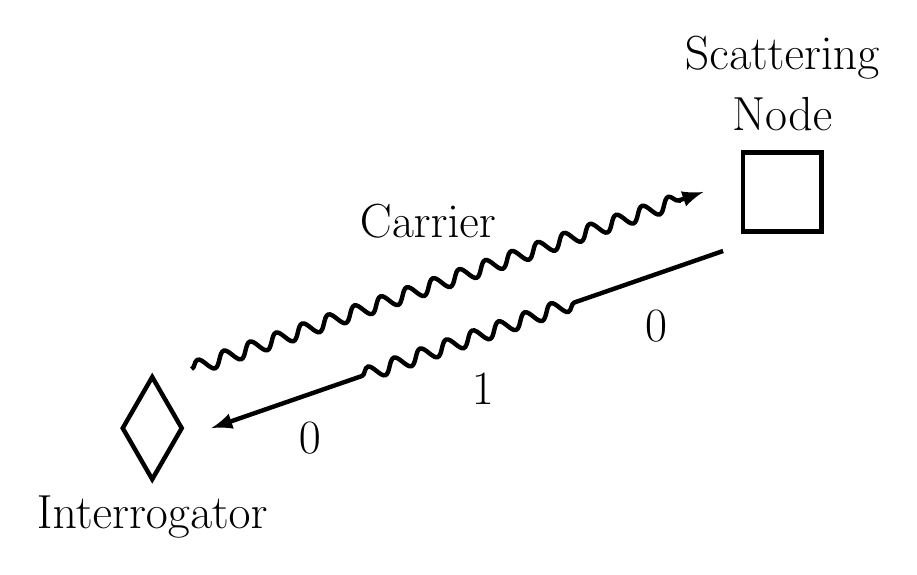
\begin{tikzpicture}[font=\LARGE,every node/.style={draw,ultra thick},every path/.style={ultra thick},every text node part/.style={align=center}]
	\node at (0,0) [kite,minimum size=0.75cm,kite vertex angles=60] {};
	\node at (8,3) [rectangle,minimum size=1cm] {};

	\node[draw=none] at (0,-1.125) {Interrogator};
	\node[draw=none] at (8,4.375) {Scattering\\Node};

	\draw[decorate,decoration={snake,post length=2.5mm},-latex] (0.5,0.75) -- (7,3);
	\draw[decorate,decoration={snake,pre length=2cm,post length=2cm},-latex] (7.25,2.25) -- (0.75,0);

	\node[draw=none] at (3.5,2.625) {Carrier};
	\node[draw=none] at (4.2,0.5) {1};
	\node[draw=none] at (2,-0.125) {0};
	\node[draw=none] at (6.4,1.3) {0};
\end{tikzpicture}

			}
			\label{fg:mbc}
		}
		\subfloat[\gls{bbc}]{
			\resizebox{0.48\linewidth}{!}{
				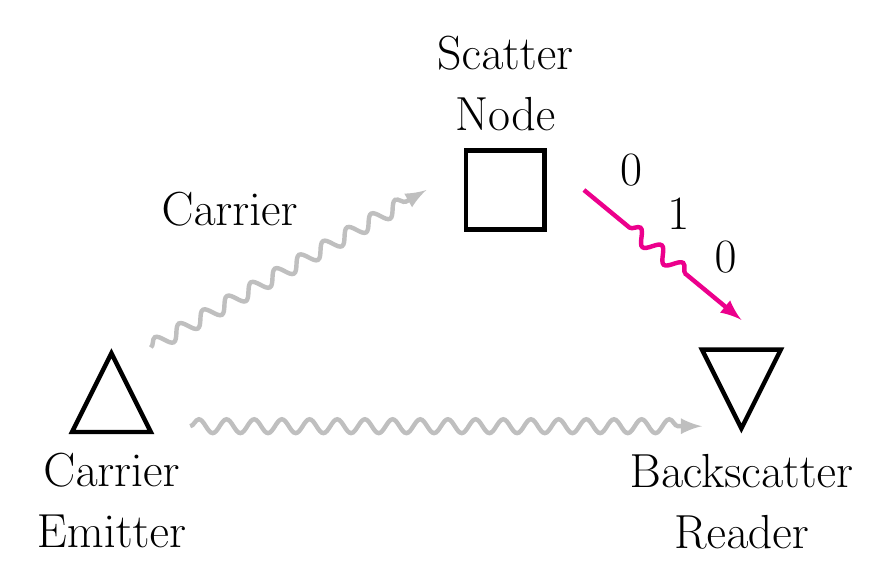
\begin{tikzpicture}[font=\LARGE,every node/.style={draw,ultra thick},every path/.style={ultra thick},every text node part/.style={align=center}]
	\node at (0,0) [isosceles triangle,isosceles triangle stretches,shape border rotate=+90,minimum size=1cm,minimum height=1cm,anchor=north] {};
	\node at (5,2) [rectangle,minimum size=1cm] {};
	\node at (8,0) [isosceles triangle,isosceles triangle stretches,shape border rotate=+270,minimum size=1cm,minimum height=1cm,anchor=north] {};

	\node[draw=none] at (0,-1.95) {Carrier\\Emitter};
	\node[draw=none] at (5,3.35) {Scatter\\Node};
	\node[draw=none] at (8,-1.95) {Backscatter\\Reader};

	\draw[lightgray,decorate,decoration={snake,post length=2.5mm},-latex] (1,-1) -- (7.5,-1);
	\draw[lightgray,decorate,decoration={snake,post length=2.5mm},-latex] (0.5,0) -- (4,2);
	\draw[magenta,decorate,decoration={snake,pre length=7.5mm,post length=7.5mm},-latex] (6,2) -- (8,0.35);

	\node[draw=none] at (1.5,1.75) {Carrier};
	\node[draw=none] at (7.2,1.7) {1};
	\node[draw=none] at (6.6,2.25) {0};
	\node[draw=none] at (7.8,1.15) {0};
\end{tikzpicture}

			}
			\label{fg:bbc}
		}
		\\
		\subfloat[\gls{ambc}]{
			\resizebox{0.48\linewidth}{!}{
				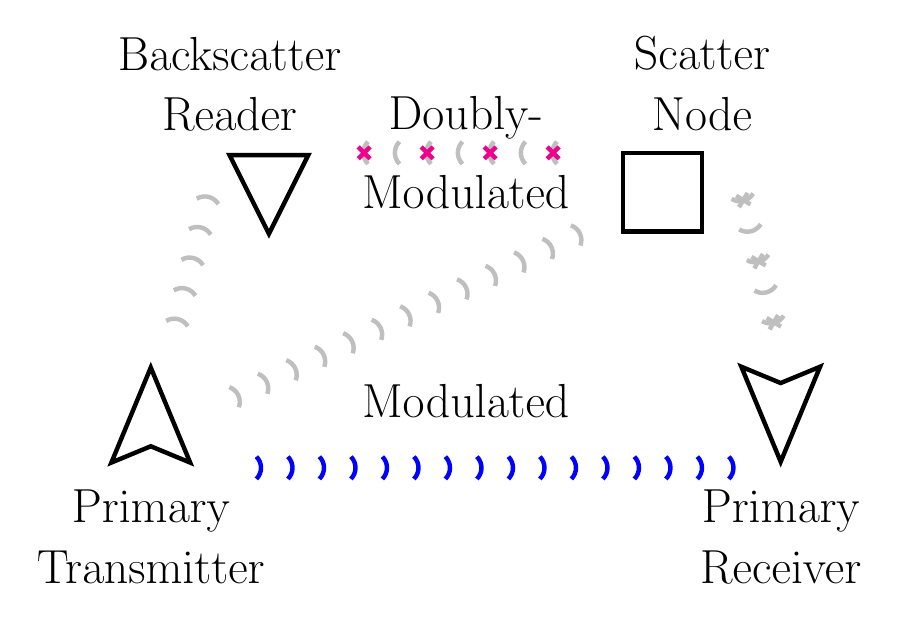
\begin{tikzpicture}[font=\LARGE,every node/.style={draw,ultra thick},every path/.style={ultra thick},every text node part/.style={align=center}]
	\node at (0,0) [dart,shape border rotate=90,minimum width=1cm] {};
	\node at (1.5,3.5) [isosceles triangle,isosceles triangle stretches,shape border rotate=+270,minimum size=1cm,minimum height=1cm,anchor=north] {};
	\node at (6.5,3) [rectangle,minimum size=1cm] {};
	\node at (8,0.35) [dart,shape border rotate=270,minimum width=1cm] {};

	\node[draw=none] at (0,-1.375) {Primary\\Transmitter};
	\node[draw=none] at (1,4.375) {Backscatter\\Reader};
	\node[draw=none] at (7,4.375) {Scatter\\Node};
	\node[draw=none] at (8,-1.375) {Primary\\Receiver};

	\draw[blue,decorate,decoration={waves,segment length=4mm,radius=2mm}] (1,-0.5) -- (7.5,-0.5);
	\draw[lightgray,decorate,decoration={waves,segment length=4mm,radius=2mm}] (0.25,1) -- (0.75,3);
	\draw[lightgray,decorate,decoration={waves,segment length=4mm,radius=2mm}] (0.75,0.25) -- (5.5,2.5);
	\draw[lightgray,decorate,decoration={waves,segment length=4mm,radius=2mm}] (5.5,3.5) -- (2.5,3.5);
	\draw[magenta,decorate,decoration={crosses,segment length=8mm,shape size=1.5mm}] (5.11,3.5) -- (2.5,3.5);
	\draw[lightgray,decorate,decoration={waves,segment length=4mm,radius=2mm}] (7.43,3.28) -- (8,1);
	\draw[lightgray,decorate,decoration={crosses,segment length=8mm,shape size=1.5mm}] (7.525,2.9) -- (8,1);

	\node[draw=none] at (4,0.35) {Modulated};
	\node[draw=none] at (4,3.95) {Doubly-};
	\node[draw=none] at (4,3) {Modulated};
\end{tikzpicture}

			}
			\label{fg:ambc}
		}
		\subfloat[\gls{sr}]{
			\resizebox{0.48\linewidth}{!}{
				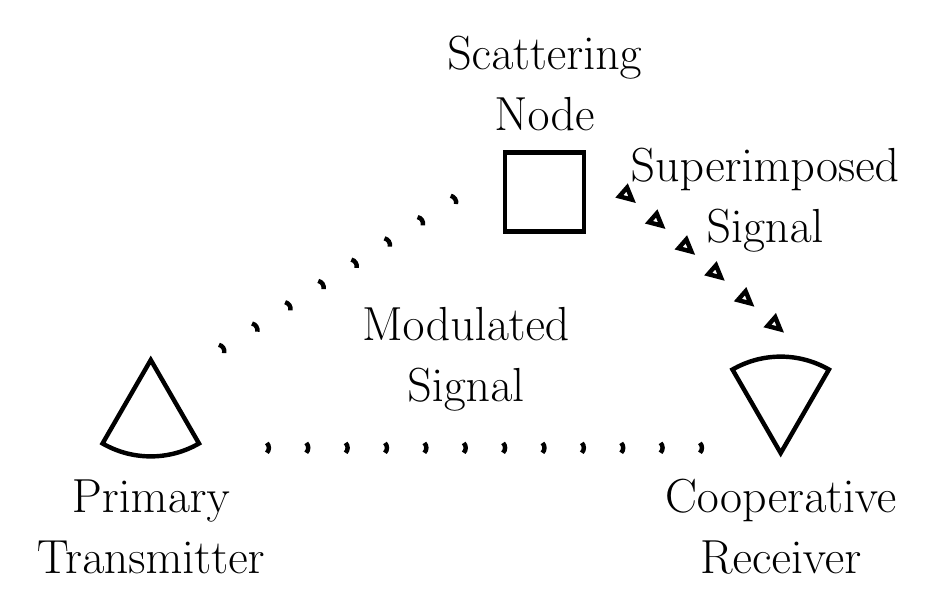
\begin{tikzpicture}[font=\LARGE,every node/.style={draw,ultra thick},every path/.style={ultra thick},every text node part/.style={align=center}]
	\node at (0,0) [circular sector,shape border rotate=90,minimum width=2cm] {};
	\node at (5,3) [rectangle,minimum size=1cm] {};
	\node at (8,0.55) [circular sector,shape border rotate=270,minimum width=2cm] {};

	\node[draw=none] at (0,-1.25) {Primary\\Transmitter};
	\node[draw=none] at (5,4.375) {Scattering\\Node};
	\node[draw=none] at (8,-1.25) {Cooperative\\Receiver};

	\draw[decorate,decoration={waves,segment length=5mm}] (1,-0.25) -- (7.375,-0.25);
	\draw[decorate,decoration={waves,segment length=5mm}] (0.5,0.75) -- (4,3);
	\draw[decorate,decoration={triangles,segment length=5mm,shape size=1.5mm}] (6,3) -- (8,1.25);

	\node[draw=none] at (4,0.875) {Modulated\\Signal};
	\node[draw=none] at (7.8,2.9) {Superimposed\\Signal};
\end{tikzpicture}

			}
			\label{fg:sr}
		}
		\\
		\subfloat[\gls{ris}]{
			\resizebox{0.48\linewidth}{!}{
				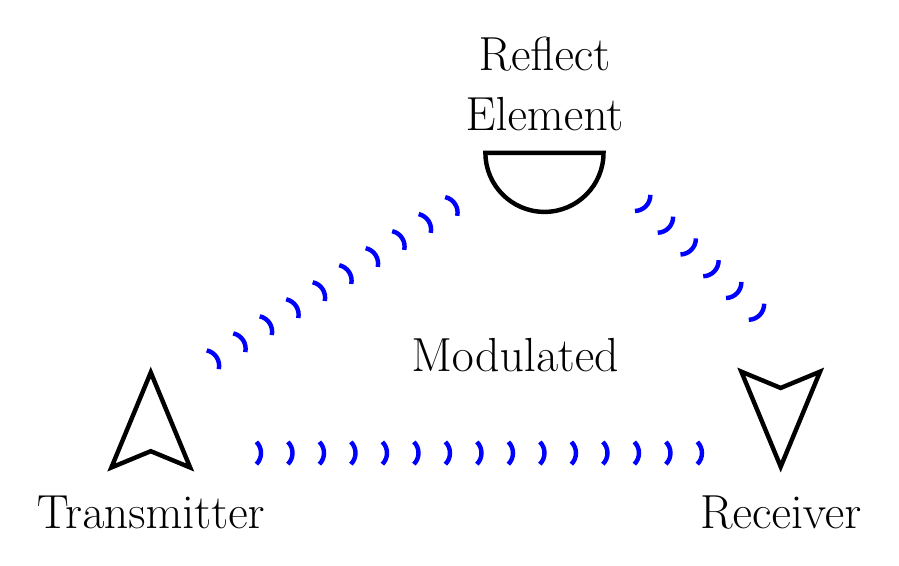
\begin{tikzpicture}[font=\LARGE,every node/.style={draw,ultra thick},every path/.style={ultra thick},every text node part/.style={align=center}]
	\node at (0,0) [dart,shape border rotate=90,minimum width=1cm] {};
	\node at (5,3.25) [semicircle,shape border rotate=180,minimum width=1.5cm] {};
	\node at (8,0.35) [dart,shape border rotate=270,minimum width=1cm] {};

	\node[draw=none] at (0,-1) {Transmitter};
	\node[draw=none] at (5,4.4375) {Reflect\\Element};
	\node[draw=none] at (8,-1) {Receiver};

	\draw[blue,decorate,decoration={waves,segment length=4mm,radius=2mm}] (1,-0.25) -- (7.375,-0.25);
	\draw[blue,decorate,decoration={waves,segment length=4mm,radius=2mm}] (0.5,0.75) -- (4,3);
	\draw[blue,decorate,decoration={waves,segment length=4mm,radius=2mm}] (6,3.1625) -- (8,1.25);

	\node[draw=none] at (4.625,1) {Modulated};
\end{tikzpicture}

			}
			\label{fg:ris}
		}
		\subfloat[RIScatter]{
			\resizebox{0.48\linewidth}{!}{
				\begin{tikzpicture}[every node/.style={draw}]
	\node at (0,0) [dart,shape border rotate=90,minimum width=1cm] {};
	\node at (7,4) [circle,minimum size=1cm] {};
	\node at (10,0.35) [dart,shape border rotate=270,minimum width=1cm] {};

	\node[draw=none] at (0,-0.75) {Primary Transmitter};
	\node[draw=none] at (7,5) {RIScatter Node};
	\node[draw=none] at (10,-0.75) {Cooperative Receiver};
	\draw[loosely dashed,-latex] (0.75,0) -- (9.25,0);
	\draw[loosely dashed,-latex] (0.5,0.5) -- (6.25,4);
	\draw[dashdotted,-latex] (7.75,4) -- (10,1);
\end{tikzpicture}

			}
			\label{fg:riscatter}
		}
		\caption{
			Illustration of scattering applications.
			The blue flow(s) constitutes the primary link while the magenta/green flow denotes the backscatter link.
		}
		\label{fg:scatter_illustration}
	\end{figure}
	% \end{subsection}

	\begin{table*}[!t]
		\caption{Comparison of Scattering Applications}
		\label{tb:scattering_applications}
		\rowcolors{2}{gray!25}{white}
		\renewcommand{\arraystretch}{1.4}
		\begin{tabularx}{\textwidth}{CCCCCC}
			\toprule
			\hiderowcolors
			                                       & \gls{mbc}/\gls{bbc} & \gls{ambc}                  & \gls{sr} (large spreading factor)               & \gls{ris}           & RIScatter                                                   \\ \midrule
			\showrowcolors
			Information link(s)                    & Backscatter         & Coexisting                  & Coexisting                                      & Primary             & Coexisting                                                  \\
			Primary signal on backscatter decoding & Carrier             & Multiplicative interference & Spreading code                                  & ---                 & Energy uncertainty                                          \\
			Backscatter signal on primary decoding & ---                 & Multiplicative interference & \gls{csi} uncertainty                           & Passive beamforming & Dynamic passive beamforming                                 \\
			Cooperative devices                    & ---                 & No                          & Primary transmitter and co-located receiver     & ---                 & Primary transmitter, scatter nodes, and co-located receiver \\
			Sequential decoding                    & ---                 & No                          & Primary-to-backscatter, \gls{sic} and \gls{mrc} & ---                 & Backscatter-to-primary, no \gls{sic}/\gls{mrc}              \\
			% Primary decoding                        & ---                 & Semi-coherent               & Semi-coherent                                   & Coherent            & Coherent                                                    \\
			% Backscatter decoding                    & Coherent            & Semi-coherent               & Coherent                                        & ---                 & Semi-coherent                                               \\
			Reflection pattern depends on          & Information source  & Information source          & Information source                              & \gls{csi}           & Information source, \gls{csi}, and \gls{qos}                \\
			Reflection state distribution          & Equiprobable        & Equiprobable                & Equiprobable or Gaussian                        & Degenerate          & Flexible                                                    \\
			Load-switching speed                   & Fast                & Slow                        & Slow                                            & Quasi-static        & Arbitrary                                                   \\ \bottomrule
		\end{tabularx}
	\end{table*}

	% \begin{subsection}{Related Works}
	As a special case of \gls{cr}, active and passive transmissions coexist and interplay in \gls{ambc} and \gls{sr}.
	Such a coexistence is classified into commensal (overlay), parasitic (underlay), and competitive paradigms, and their achievable rate and outage performance were investigated in \cite{Guo2019b,Ding2020}.
	For the co-located cooperative receiver, the \gls{ber} performance of \gls{ml}, linear, and \gls{sic} detectors are derived over flat fading channels \cite{Yang2018}.
	However, the work assumed equal symbol period and perfect synchronization for primary and backscatter links.
	Importantly, active-passive coexisting networks have three special and important properties:
	\begin{enumerate}
		\item Primary and backscatter symbols are superimposed by \emph{double modulation} (i.e., multiplication coding);
		\item Backscatter signal strength is much weaker than primary due to the \emph{double fading} effect;
		\item The spreading factor (i.e., backscatter symbol period over primary) is usually large\footnote{The load-switching interval of low-power backscatter modulators is usually \num{0.1} to \qty{10}{\us} \cite{Torres2021}, accounting for a typical spreading factor between \num{10} and \num{e3}.}.
	\end{enumerate}
	The second property motivated \cite{Long2020a,Liang2020,Guo2019b,Ding2020,Zhou2019a,Wu2021a,Xu2021a,Yang2021a,Yang2018,Han2021,Zhang2022} to view \gls{sr} as a multiplicative \gls{noma} and perform \gls{sic} from primary to backscatter link.
	During primary decoding, the backscatter signal can be modelled as channel uncertainty or multiplicative interference when the spreading factor is large or small, respectively.
	Decoding each backscatter symbol also requires multiple \gls{sic} followed by a \gls{mrc} and is operation-intensive and \gls{csi}-sensitive.
	% Such a \gls{sic} receiver is operation-intensive and \gls{csi}-sensitive because it involves $N$ re-encoding, precoding, subtraction together with a time-domain \gls{mrc} to decode each backscatter symbol.
	When the spreading factor is sufficiently large, the primary achievable rate under semi-coherent detection\footnote{In this paper, semi-coherent detection refers to the primary/backscatter decoding with known \gls{csi} and unknown backscatter/primary symbols.} asymptotically approaches its coherent counterpart and both links are decoded interference-free \cite{Long2020a}.
	% However, it significantly increases \gls{sic} operations per backscatter symbol and severely limits the backscatter \emph{throughput}.
	However, it severely limits the backscatter throughput and requires more \gls{sic} per backscatter symbol.

	% On the other hand, efficient backscatter multiple access design remains an open issue for \gls{bc}.
	% \cite{Xu2021a} proposed a \gls{noma}-based \gls{sr} where the \gls{sic} order depends on the backscatter channel strength, but the performance deteriorates fast as the number of nodes increases.
	% \gls{tdma}-based \gls{sr} was also considered in \cite{Yang2021a} where each node transmits information during its dedicated slot and harvests energy otherwise.
	% It enables adaptive transmission time and reflection ratio design but introduces extra coordination cost.
	% \cite{Vougioukas2019} modifies the load-switching speed to shift the scattered signal to the desired frequency band.
	% This enables backscatter \gls{fdma} at the cost of larger bandwidth and higher power consumption at the scatter nodes.
	% To reduce the coordination cost, \cite{Han2021} proposed a random code-assisted multiple access for \gls{sr} and evaluated the asymptotic \gls{sinr} using random matrix theory.
	% This code-domain solution suffers from the near-far problem and imperfect synchronization, both being severe in \gls{bc}.

	% A comparison of scattering applications is summarized in Table~\ref{tb:scattering_applications}.

	On the other hand, static \gls{ris} design with fixed reflection pattern per channel block has been extensively studied in wireless communication, sensing, and power literature \cite{Wu2018,Zhang2019a,Lin2022,Liu2022,Feng2022,Zhao2022}.
	Dynamic \gls{ris} performs time sharing between different phase shifts and introduces artificial channel diversity within each channel block.
	It was first proposed to fine-tune the \gls{ofdm} resource blocks \cite{Yang2020} then extended to the downlink power and uplink information phases of \gls{wpcn} \cite{Wu2021,Wu2021d,Hua2022a}.
	However, dynamic \gls{ris} carries no information since the reflection state at each time slot is known to the receiver.
	\gls{ris} can also be used as an index-modulated information source and prototypes are already available for \gls{psk} \cite{Tang2019a} and \gls{qam} \cite{Dai2020a}.
	From an information-theoretic perspective, the authors of \cite{Karasik2020} reported that joint transmitter-\gls{ris} encoding achieves the capacity of \gls{ris}-aided finite-input channel and using \gls{ris} as a naive passive beamformer to maximize the receive \gls{snr} is generally suboptimal.
	This inspired \gls{ris}-empowered \gls{bc} \cite{Liu2019d,Bereyhi2020,Xu2020b,Zhang2021d,Hu2021b,Hua2022,Basar2020,Ma2020a,Yuan2021,Hu2021a} to combine passive beamforming and backscatter modulation in the overall reflection pattern.
	In particular, \emph{symbol level precoding} maps the information symbols to the optimized \gls{ris} coefficient sets \cite{Liu2019d,Bereyhi2020}, \emph{overlay modulation} superposes the information symbols over a common auxiliary matrix \cite{Xu2020b,Zhang2021d,Hu2021b,Hua2022}, \emph{spatial modulation} switches between the reflection coefficient sets that maximize \gls{snr} at different receive antennas \cite{Basar2020,Ma2020a,Yuan2021}, and \emph{index modulation} employs dedicated reflection elements (resp. information elements) for passive beamforming (resp. backscatter modulation) \cite{Hu2021a}.
	However, those joint designs incur advanced hardware architecture and high optimization complexity.
	Relevant literature also considers either Gaussian codebook \cite{Guo2019b,Ding2020,Long2020a,Zhou2019a,Wu2021a,Xu2021a,Yang2021a,Hu2021b} that is impractical for low-power nodes or finite equiprobable inputs \cite{Yang2018,Liang2020,Han2021,Zhang2022,Liu2019d,Bereyhi2020,Xu2020b,Zhang2021d,Hua2022,Basar2020,Ma2020a,Yuan2021,Hu2021a} that does not fully exploit the \gls{csi} and properties of active-passive coexisting networks.
	% \end{subsection}
	Those problems are addressed in this paper and the contributions are summarized below.

	% \begin{subsection}{Contributions}
	% \emph{First,} we propose RIScatter as a novel scatter protocol that unifies \gls{bc} and \gls{ris} by adaptive reflection state (backscatter input) distribution design.
	% \emph{First,} we propose RIScatter as a novel scatter protocol that simultaneously modulates the nodes information and engineers the wireless channel via adaptive reflection state (backscatter input) distribution design.
	\emph{First,} we propose RIScatter as a novel scatter protocol that simultaneously modulates the node information and engineers the wireless channel via adaptive reflection state (backscatter input) distribution design.
	The concept is shown in Fig.~\subref*{fg:riscatter} where the message of one or more RIScatter nodes and a primary transmitter are sequentially decoded by a co-located receiver.
	% The reflection pattern is random with the guidance of input distribution as a joint function of the information source, \gls{csi}, and \gls{qos}
	% The reflection pattern is a discrete random variable with probability mass function
	% (co-located or dispersed)
	Each reflection state simultaneously acts as an information codeword and a passive beamforming codeword.
	The reflection pattern of each node is randomly chosen with the guidance of input distribution that is designed as a joint function of the information source, \gls{csi}, and \gls{qos}.
	% That is, each reflection state simultaneously acts as information codeword and passive beamforming codeword (symbol-level passive precoding).
	% Since each reflection state simultaneously acts as information codeword and passive beamforming codeword (symbol-level passive precoding).
	Such an adaptive channel coding boils down to the degenerate distribution of \gls{ris} when the primary link is prioritized, and outperforms the uniform distribution of line-coded \gls{bc} (by accounting the \gls{csi}) when the backscatter link is prioritized.
	% Joint and independent encoding are available when multiple RIScatter nodes are
	Multiple RIScatter nodes can be co-located with joint encoding or dispersed with independent encoding.
	% The reflection state is neither fully random (cf. \gls{bc}) nor fully deterministic (cf. \gls{ris}), but semi-random in reflection state distribution.
	% RIScatter exploits the transmitter-scatter-receiver path for simultaneous backscatter modulation and dynamic passive beamforming, and can smoothly transition in between under different \gls{qos}.
	% A comparison of RIScatter to \gls{bc} and \gls{ris} is summarized in Table~\ref{tb:scattering_applications}.
	Table~\ref{tb:scattering_applications} compares RIScatter to \gls{bc} and \gls{ris}.
	However, two major challenges for RIScatter are the cooperative receiver design and the backscatter input distribution design.
	% such a novel scatter protocol encounters two major challenges, namely the cooperative receiver design and the adaptive backscatter input distribution design.
	This is the first paper to unify \gls{bc} and \gls{ris} from the perspective of input distribution.

	\emph{Second,} we address the first challenge and propose a practical receiver that semi-coherently decodes the backscatter information, recovers the exact reflection pattern (and composite channel), and coherently decodes the primary link.
	% Energy detection is used to decode the multiplicative backscatter information under primary uncertainty, and disjoint decision regions are formulated
	% Energy detection is used to decode the multiplicative backscatter information under primary uncertainty, and it divides the accumulated energy domain into disjoint decision regions to construct \gls{dmc}
	% Energy detection is used for backscatter decoding that
	We consider backscatter energy detection with disjoint decision regions and formulates a \gls{dmtmac}.
	% Specifically, energy detection
	to decode the multiplicative backscatter information under primary uncertainty, and it divides the accumulated energy domain into disjoint decision regions to construct \gls{dmc}
	% , and we design disjoint detection regions to transform the \gls{dcmc} channel to \gls{dmtc}


	Hence, the receiver can semi-coherently (under primary uncertainty) decode RIScatter nodes from the accumulated receive energy, re-encode to recover the exact reflection patterns, and combine those with cascaded \gls{csi} to determine the multipath response and model within the primary channel.
	Such a backscatter-primary decoding enables simultaneous backscatter modulation and dynamic passive beamforming by only one energy comparison and re-encoding during each backscatter (instead of primary) block.

	exploits the properties of active-passive coexisting networks and
	% \emph{Second,} we address the first challenge and propose a practical receiver that exploits the three properties

	It semi-coherently decodes the backscatter information, recovers the exact reflection pattern, and coherently decodes the primary link.
	Thanks to the double modulation effect, once the multiplicative backscatter information is successfully decoded, the contribution is modelled within channel as dynamic passive beamforming rather than re-precoded and cancelled.

	% The semi-coherent backscatter decoding is based on
	% For the semi-coherent backscatter decoding, we
	% Specifically, the backscatter decoding relys on energy
	% we transform the discrete-input continuous-output backscatter channel
	We use energy detection to decode the multiplicative backscatter information under primary uncertainty, and transform the

	we transform the discrete-input continuous-output backscatter channel
	the energy space is divided into disjoint decision regions associated with different hypothese
	% Double modulation enables symbol-level passive precoding such that the
	The multiplicative backscatter information, once successfully decoded, can be modelled as dynamic passive beamforming (rather than being re-precoded and cancelled) and thus the energy detection becomes part of channel training.
	The proposed receiver significantly improves backscatter throughput since it is suitable for arbitrary input distribution and spreading factor.
	This is the first paper to consider practical backscatter-primary decoding scheme at the co-located receiver.

	\emph{Third,} we address the second challenge and

	by considering a specific scenario where multiple co-located/dispersed RIScatter nodes ride over an active point-to-point \gls{miso} transmission to perform backscatter modulation and dynamic passive beamforming towards a nearby user.
	For a given \gls{qos}, we first express the primary and total backscatter rates as functions of \emph{input distribution} at RIScatter nodes, \emph{active beamforming} at the \gls{ap}, and \emph{backscatter decision regions} at the user.
	Then, we characterize the achievable rate region by optimizing those variables under different \gls{qos}.
	Since the original problem is highly non-convex, we propose a suboptimal \gls{bcd} algorithm where the \gls{kkt} input distribution is numerically evaluated by limit of sequences, the active beamforming is iteratively updated by \gls{pgd} accelerated by \gls{bls}, and the decision regions are refined by existing sequential quantization methods for \gls{dmtc}.
	Uniquely, we account for \gls{csi}, \gls{qos}, and backscatter constellation in those optimizations, and the proposed backscatter input distribution design is applicable to more general scenarios.
	This is also the first paper to reveal the importance of backscatter input distribution and decision region designs in active-passive coexisting networks.

	% \emph{Fourth,} we provide numerical results to demonstrate the benefits of RIScatter and proposed algorithms.
	% The observations include:
	% 1) adaptive reflection state distribution design can flexibly shift between backscatter modulation and passive beamforming;
	% 2) when the primary link is prioritized, input distribution becomes degenerate and RIScatter nodes coincide with discrete \gls{ris};
	% 3) when the backscatter link is prioritized, adaptive RIScatter encoding achieves higher backscatter rate than conventional line-coded \gls{bc} with equiprobable inputs;
	% 4) co-located RIScatter nodes can further leverage total backscatter rate by joint encoding;
	% 5) the proposed receiver maintains the passive beamforming benefit and provides comparable backscatter rate to \gls{sic}-based \gls{sr}, with re-encoding costs reduced to $1/N$ and no re-precoding/cancellation;
	% 6) it also supports scatter nodes with faster load-switching speed for potentially higher throughput;
	% 7) \gls{pgd} active beamformer effectively increases the primary (resp. backscatter) rate by boosting the receive \gls{snr} (resp. widening the energy gap under different reflection states), and can smoothly transition in between under different \gls{qos};
	% 8) distribution-aware backscatter detectors provide higher backscatter rate than the conventional \gls{ml} detector.
	% \end{subsection}

	\emph{Notations:}
	Italic, bold lower-case, and bold upper-case letters denote scalars, vectors and matrices, respectively.
	$\boldsymbol{0}$ and $\boldsymbol{1}$ denote zero and one array of appropriate size, respectively. $\mathbb{I}^{x \times y}$, $\mathbb{R}_+^{x \times y}$, and $\mathbb{C}^{x \times y}$ denote the unit, real nonnegative, and complex spaces of dimension $x \times y$, respectively.
	$j$ denotes the imaginary unit.
	$\mathrm{diag}(\cdot)$ returns a square matrix with the input vector on its main diagonal and zeros elsewhere.
	$\mathrm{card}(\cdot)$ returns the cardinality of a set.
	$(\cdot)^*$, $(\cdot)^\mathsf{T}$, $(\cdot)^\mathsf{H}$, $\lvert{\cdot}\rvert$, and $\lVert{\cdot}\rVert$ denote the conjugate, transpose, conjugate transpose (Hermitian), absolute value, and Euclidean norm operators, respectively.
	$(\cdot)^{(r)}$ and $(\cdot)^{\star}$ denote the $r$-th iterated and optimal results, respectively.
	The distribution of a \gls{cscg} random variable with zero mean and variance $\sigma^2$ is denoted by $\mathcal{CN}(0,\sigma^2)$, and $\sim$ means ``distributed as''.
\end{section}

\begin{section}{Scattering Principles}
	\gls{rf} wave scattering and reflecting can be described by a unified model and realized by {variable-load antennas} or {programmable metamaterial} \cite{Liang2022}.
	An antenna-based scatterer usually consists of an integrated antenna, a load-switching modulator, an energy harvester, and on-chip components (e.g., microcontroller and sensors) \cite{Dobkin2012}.
	It first receives the impinging signals, then reradiates some back to the space and dissipates the remaining.
	In comparison, a typical metamaterial-based scatterer comprises an outer metamaterial layer of numerous sub-wavelength metallic/dielectric patches (with tunable permittivity/permeability), a middle copper plate layer that avoids leakage, an inner circuit board layer that adjusts patch responses, and an integrated microcontroller/\glsentryshort{fpga} for coordination and control \cite{Wu2020}.
	Ideally, it reflects the wave at the space-metamaterial boundary without receiving them and mainly applies a phase shift.
	In practice, both types of scatterers have {finite} reflection states with non-zero reflection loss.
	The scattered signal can be decomposed into a {structural} mode component that consistently contributes to environment multipath and can be modelled within \gls{csi}, and an \emph{antenna} mode component that depends on the impedance mismatch and can be used for backscatter modulation and/or passive beamforming \cite{Hansen1989}.
	For an antenna-based (resp. metamaterial-based) scatter node with $M$ reflection states, the reflection coefficient at state $m \in \mathcal{M} \triangleq \{1,\ldots,M\}$ is
	\begin{equation}
		\Gamma_m = \frac{Z_m - Z^*}{Z_m + Z},
		\label{eq:reflection_coefficient}
	\end{equation}
	where $Z_m$ is the antenna load (resp. metamaterial unit) impedance at state $m$ and $Z$ is the antenna input (resp. medium characteristic) impedance.
	\gls{bc} employ scatter nodes as information sources that \emph{randomly switching} between different states.
	For $M$-ary \gls{qam}, constellation point $c_m$ maps to reflection coefficient $\Gamma_m$ by \cite{Thomas2012a}
	\begin{equation}
		\Gamma_m = \alpha \frac{c_m}{\max_{m'} \lvert c_{m'} \rvert},
		\label{eq:backscatter_modulation}
	\end{equation}
	where $\alpha \in \mathbb{I}$ is the common amplitude scattering ratio at the direction of interest.
	In contrast, \gls{ris} employ reflect elements as channel adaptors that \emph{deterministically choosing} the reflection state based on \gls{csi}.
	For a \gls{ris} element with $M$ available states, phase shift $\theta_m$ maps to reflection coefficient $\Gamma_m$ by \cite{Wu2018}
	\begin{equation}
		\Gamma_m = \beta_m \exp(j \theta_m),
		\label{eq:passive_beamforming}
	\end{equation}
	where $\beta_m \in \mathbb{I}$ is the overall amplitude scattering ratio at state $m$.\footnote{Most existing \gls{ris} literature assumes lossless reflection $\beta_m=1$, $\forall m$.}
\end{section}

\begin{section}{RIScatter}
	\begin{subsection}{Concepts}
		We propose RIScatter in Fig.~\subref*{fg:riscatter} as a generalization of \gls{bc} and \gls{ris}, which involves coexisting active primary and passive backscatter links in a flexible and mutualistic manner.
		RIScatter nodes leverage \gls{csi}- and \gls{qos}-based reflection state distribution design to smoothly shift between backscatter modulation and passive beamforming.
		Fig.~\ref{fg:riscatter_node} illustrates the block diagram, equivalent circuit, and scatter model of a RIScatter node.
		It can be implemented by adding an integrated receiver \cite{Kim2021a} and adaptive encoder \cite{He2020e} to off-the-shelf passive \gls{rfid} tags.
		\begin{figure*}[!t]
			\centering
			\subfloat[Block Diagram]{
				\resizebox{0.32\linewidth}{!}{
					\makeatletter
\tikzset{
	block/.style={draw,rectangle,align=center},
	from/.style args={#1 to #2}{
			above right={0cm of #1},
			/utils/exec=\pgfpointdiff
			{\tikz@scan@one@point\pgfutil@firstofone(#1)\relax}
			{\tikz@scan@one@point\pgfutil@firstofone(#2)\relax},
			minimum width/.expanded=\the\pgf@x,
			minimum height/.expanded=\the\pgf@y
		}
}
\makeatother

\begin{circuitikz}[transform shape]
	\tikzstyle{every node}=[font=\small]
	\coordinate (O) at (0,0);
	\node[block,from={O to $(O) + (6.375,3)$}](T){};
	\draw (0,1.5)
	to[short] ++(-0.875,0)
	to[short] ++(0,0.5) node[bareantenna](A){Bx};
	\draw (0,1.5)
	to[short,-*] ++(0.25,0) coordinate(J);
	\draw (J)
	to[short] ++(0,1)
	to[short] ++(0.5,0) coordinate(J1);
	\node[block,from={$(J1) + (0,-0.25)$ to $(J1) + (2.5,0.25)$}](R){Rectifier};
	\draw (J)
	to[short] ++(0.5,0) coordinate(J2);
	\node[block,from={$(J2) + (0,-0.25)$ to $(J2) + (2.5,0.25)$}](D){Demodulator};
	\draw (J)
	to[short] ++(0,-1)
	to[short] ++(0.5,0) coordinate(J3);
	\node[block,from={$(J3) + (0,-0.25)$ to $(J3) + (2.5,0.25)$}](M){Modulator};
	\draw[dashed,-{Latex[length=2mm]}] (R.east) -- ++(0.75,0);
	\draw[-{Latex[length=2mm]}] (D.east) -- ++(0.75,0);
	\draw[{Latex[length=2mm]}-] (M.east) -- ++(0.75,0);
	\node[block,from={$(R.east) + (0.75,-0.25)$ to $(R.east) + (2.875,0.25)$}](P){Power Buffer};
	\node[block,from={$(M.east) + (0.75,-0.25)$ to $(D.east) + (2.875,0.25)$}](S){Digital\\Section};
	\draw[dashed,-{Latex[length=2mm]}] (P.south) to (S.north);
	\coordinate (F1) at ($(P.south)!0.5!(S.north)$);
	\coordinate (F2) at ($(D.east)!0.5!(S.west)$);
	\coordinate (F3) at ($(D.south)!0.5!(M.north)$);
	\draw[dashed] (F1) to (F1-|D.north);
	\draw[dashed,-{Latex[length=2mm]}] (F1-|D.north) to (D.north);
	\draw[dashed] (F1-|F2) to (F2|-F3) to (M|-F3);
	\draw[dashed,-{Latex[length=2mm]}] (M|-F3) to (M.north);
\end{circuitikz}

				}
				\label{fg:block_diagram}
			}
			\subfloat[Equivalent Circuit]{
				\resizebox{0.37\linewidth}{!}{
					\begin{circuitikz}[transform shape]
	\tikzstyle{every node}=[font=\Large]
	\draw (0,0) coordinate(O)
	to [sV,l=$V_0$] ++(0,1.5)
	to [L,l=$X_{\mathrm{A}}$] ++(0,1.5)
	to [R=$R_{\mathrm{A}}$,-*] ++(3,0) coordinate(AM)
	to [sI,l_=$I_0$,-*] ++(0,-3)
	to [short] (O);
	\draw (AM)
	to [short] ++(0.5,0)
	to [L,l=$X_m$,-*] ++(3,0) coordinate(M)
	to [R=$R_m^{\mathrm{S}}$] ++(3,0) coordinate(MH);
	\draw (M)
	to [R=$R_m^{\mathrm{P}}$,-*] ++(0,-3);
	\draw (MH)
	to [D,-*] ++(1.5,0) coordinate(H)
	to [C=$X_{\mathrm{H}}$,-*] ++(0,-3);
	\draw (H)
	to [short] ++(1.5,0)
	to [R=$R_{\mathrm{H}}$] ++(0,-3)
	to [short] (O);

	\draw [dashed] (-1.125,-0.5) rectangle (3.5,4);
	\draw [dashed] (4,-0.5) rectangle (9,4);
	\draw [dashed] (9.5,-0.5) rectangle (13.5,4);

	\draw (1.125,4.25) node[]{Antenna};
	\draw (6.5,4.25) node[]{Modulator};
	\draw (11.5,4.25) node[]{Harvester \& Chip};

	\draw (3.375,2.675) to [short] (3.375,3.175) to [short] (3.25,3.175) to [short,i_=$Z_{\mathrm{A}}$] (3.125,3.175);
	\draw (4.125,-0.125) to [short] (4.125,0.375) to [short] (4.25,0.375) to [short,i=$Z_m$] (4.375,0.375);
	\draw (9.625,-0.125) to [short] (9.625,0.375) to [short] (9.75,0.375) to [short,i=$Z_{\mathrm{H}}$] (9.875,0.375);
\end{circuitikz}

				}
				\label{fg:equivalent_circuit}
			}
			\subfloat[Scatter Model]{
				\resizebox{0.28\linewidth}{!}{
					\begin{circuitikz}[transform shape]
	\tikzstyle{every node}=[font=\large]
	\ctikzset{multipoles/rotary/arrow=both}
	\draw (0,0) node[bareantenna](bareantenna){};
	\draw (bareantenna.west) ++(-1,0) node[waves](WI){};
	\draw (WI.north east) ++(0.25,0) node{$\vec{E}_{\text{I}}$};
	\draw (WI.south east) ++(0.25,0) node{$\vec{H}_{\text{I}}$};
	\draw (bareantenna.east) ++(0.5,0) node[waves](WR){};
	\draw (WR.north east) ++(0.35,0) node{$\vec{E}_m$};
	\draw (WR.south east) ++(0.35,0) node{$\vec{H}_m$};
	\draw (bareantenna) to ++(0,-1.1) to [generic,l=$Z_{\text{A}}$,/tikz/circuitikz/bipoles/length=0.75cm] ++(2.3,0) node[rotary switch=4 in 90 wiper 30,anchor=ext center,rotate=0](SW){};
	\draw (SW.cout 1) to ++(0.625,+0.5) to [generic,/tikz/circuitikz/bipoles/length=0.75cm] ++(2.2,0) coordinate(E1);
	\draw (SW.cout 2) node[above right]{$m$} to [generic,l=$Z_m$,/tikz/circuitikz/bipoles/length=0.75cm] ++(2.2,0) coordinate(E2);
	\draw (SW.cout 3) to [generic,/tikz/circuitikz/bipoles/length=0.75cm] ++(2.2,0) coordinate(E3);
	\draw (SW.cout 4) to ++(0.625,-0.5) to [generic,/tikz/circuitikz/bipoles/length=0.75cm] ++(2.2,0) coordinate(E4);
	\draw (E1) to[short,-*] (E2);
	\draw (E2) to[short,-*] (E3);
	\draw (E3) to[short] (E4);
	\draw (E2) to[short] ++(0.2,0) node[ground,rotate=90]{};
\end{circuitikz}

				}
				\label{fg:scatter_model}
			}
			\caption{
			Block diagram, equivalent circuit, and scatter model of a RIScatter node.
			The solid and dashed vectors represent signal and energy flows.
			The scatter antenna behaves as a constant power source, where the voltage $V_0$ and current $I_0$ are introduced by incident electric field $\vec{E}_{\text{I}}$ and magnetic field $\vec{H}_{\text{I}}$ \cite{Huang2021}.
			}
			\label{fg:riscatter_node}
		\end{figure*}
		Fig.~\ref{fg:scatter_comparison} compares the reflection state distribution and reflection pattern of RIScatter and other applications.
		\begin{figure}[!t]
			\centering
			\subfloat[Reflection State Distribution]{
				\resizebox{0.8\columnwidth}{!}{
					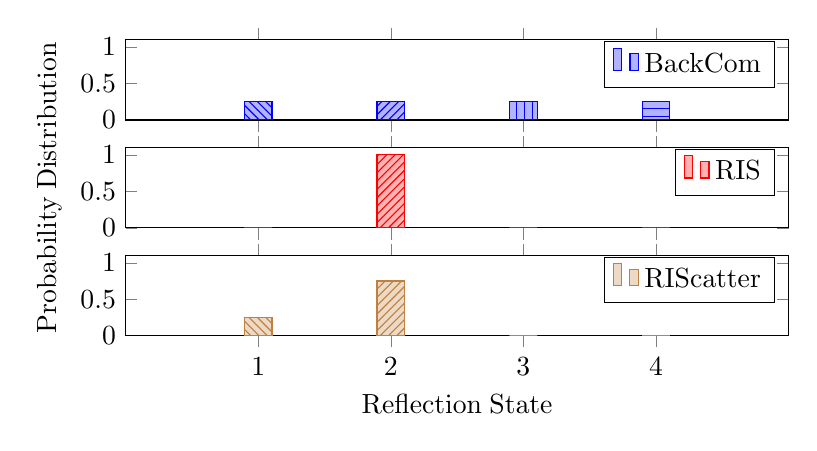
\begin{tikzpicture}
	\begin{groupplot}
		[group style={
					rows=3,
					group name=plots,
					x descriptions at=edge bottom,
					y descriptions at=edge left,
					vertical sep=10
				},
			ybar,
			xmin=0,
			xmax=4,
			xtick={1,2,3,4},
			ymin=0,
			ymax=1,
			xlabel={Reflection State},
			enlarge x limits={value=0.25,upper},
			enlarge y limits={value=0.1,upper},
			width=10cm,
			height=2.6cm,
			every axis plot/.append style={bar shift=0}
		]
		\nextgroupplot
		\addplot[blue,fill=blue!30!white] coordinates {(-1,-1)};
		\addplot[blue,fill=blue!30!white,postaction={pattern=north west lines},pattern color=.] coordinates {(1,0.25)};
		\addplot[blue,fill=blue!30!white,postaction={pattern=north east lines},pattern color=.] coordinates {(2,0.25)};
		\addplot[blue,fill=blue!30!white,postaction={pattern=vertical lines},pattern color=.] coordinates {(3,0.25)};
		\addplot[blue,fill=blue!30!white,postaction={pattern=horizontal lines},pattern color=.] coordinates {(4,0.25)};
		\legend{BackCom}
		\nextgroupplot[ylabel={Probability Distribution}]
		\addplot[red,fill=red!30!white] coordinates {(-1,-1)};
		\addplot[red,fill=red!30!white,postaction={pattern=north west lines},pattern color=.] coordinates {(1,0)};
		\addplot[red,fill=red!30!white,postaction={pattern=north east lines},pattern color=.] coordinates {(2,1)};
		\addplot[red,fill=red!30!white,postaction={pattern=vertical lines},pattern color=.] coordinates {(3,0)};
		\addplot[red,fill=red!30!white,postaction={pattern=horizontal lines},pattern color=.] coordinates {(4,0)};
		\legend{RIS}
		\nextgroupplot
		\addplot[brown,fill=brown!30!white] coordinates {(-1,-1)};
		\addplot[brown,fill=brown!30!white,postaction={pattern=north west lines},pattern color=.] coordinates {(1,0.25)};
		\addplot[brown,fill=brown!30!white,postaction={pattern=north east lines},pattern color=.] coordinates {(2,0.75)};
		\addplot[brown,fill=brown!30!white,postaction={pattern=vertical lines},pattern color=.] coordinates {(3,0)};
		\addplot[brown,fill=brown!30!white,postaction={pattern=horizontal lines},pattern color=.] coordinates {(4,0)};
		\legend{RIScatter}
	\end{groupplot}
\end{tikzpicture}

				}
				\label{fg:input_distribution}
			}
			\\
			\subfloat[Reflection Pattern]{
				\resizebox{0.8\columnwidth}{!}{
					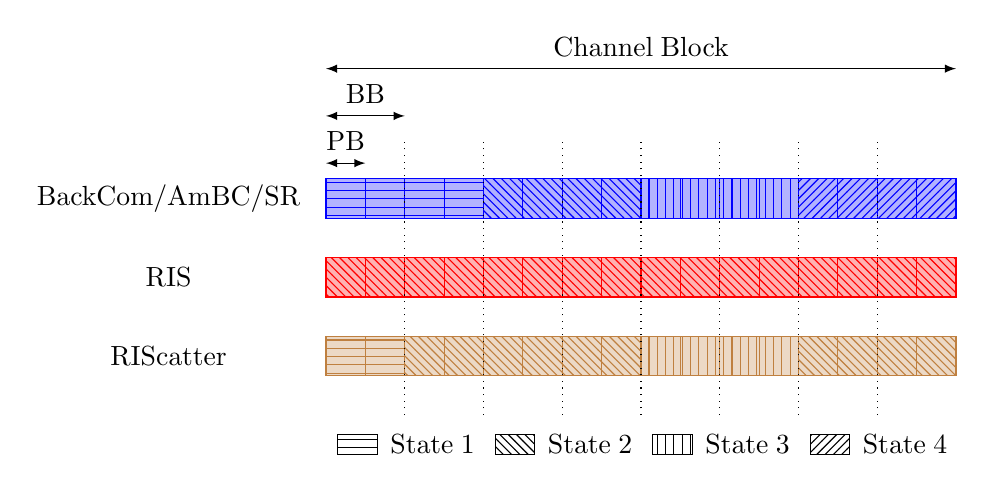
\begin{tikzpicture}
	% BC/AmBC/SR
	\foreach \x in {0,...,3}{
			\draw[blue,fill=blue!30!white,postaction={pattern=horizontal lines},pattern color=.] (0.5*\x,3) rectangle ++(0.5,0.5);
		}
	\foreach \x in {4,...,7}{
			\draw[blue,fill=blue!30!white,postaction={pattern=north west lines},pattern color=.] (0.5*\x,3) rectangle ++(0.5,0.5);
		}
	\foreach \x in {8,...,11}{
			\draw[blue,fill=blue!30!white,postaction={pattern=vertical lines},pattern color=.] (0.5*\x,3) rectangle ++(0.5,0.5);
		}
	\foreach \x in {12,...,15}{
			\draw[blue,fill=blue!30!white,postaction={pattern=north east lines},pattern color=.] (0.5*\x,3) rectangle ++(0.5,0.5);
		}

	% RIS
	\foreach \x in {0,...,15}{
			\draw[red,fill=red!30!white,postaction={pattern=north west lines},pattern color=.] (0.5*\x,2) rectangle ++(0.5,0.5);
		}

	% RIScatter
	\foreach \x in {0,...,1}{
			\draw[brown,fill=brown!30!white,postaction={pattern=horizontal lines},pattern color=.] (0.5*\x,1) rectangle ++(0.5,0.5);
		}
	\foreach \x in {2,...,7}{
			\draw[brown,fill=brown!30!white,postaction={pattern=north west lines},pattern color=.] (0.5*\x,1) rectangle ++(0.5,0.5);
		}
	\foreach \x in {8,...,11}{
			\draw[brown,fill=brown!30!white,postaction={pattern=vertical lines},pattern color=.] (0.5*\x,1) rectangle ++(0.5,0.5);
		}
	\foreach \x in {12,...,15}{
			\draw[brown,fill=brown!30!white,postaction={pattern=north west lines},pattern color=.] (0.5*\x,1) rectangle ++(0.5,0.5);
		}

	\foreach \x in {1,...,7}{
			\draw[dotted] (\x,0.5) -- (\x,4);
		}
	\draw[latex-latex] (0,3.7) -- (0.5,3.7) node[above,midway,yshift=1]{PB};
	\draw[latex-latex] (0,4.3) -- (1,4.3) node[above,midway,yshift=1]{BB};
	\draw[latex-latex] (0,4.9) -- (8,4.9) node[above,midway,yshift=1]{Channel Block};

	\node at (-2,3.25) {BackCom/AmBC/SR};
	\node at (-2,2.25) {RIS};
	\node at (-2,1.25) {RIScatter};

	\draw [pattern=horizontal lines](0.15,0) rectangle ++(0.5,0.25) node[xshift=20,yshift=-3.5] {State 1};
	\draw [pattern=north west lines](2.15,0) rectangle ++(0.5,0.25) node[xshift=20,yshift=-3.5] {State 2};
	\draw [pattern=vertical lines](4.15,0) rectangle ++(0.5,0.25) node[xshift=20,yshift=-3.5] {State 3};
	\draw [pattern=north east lines](6.15,0) rectangle ++(0.5,0.25) node[xshift=20,yshift=-3.5] {State 4};
\end{tikzpicture}

				}
				\label{fg:time_structure}
			}
			\caption{
				Reflection state distribution and reflection pattern over time of scattering applications.
				``PB'', ``BB'', and ``CB'' refer to primary block, backscatter block, and channel block, respectively.
				\gls{bc} employs all possible states as information codewords, \gls{ris} treats them as beamformer codewords, and RIScatter simultaneously exploits both benefits.
			}
			\label{fg:scatter_comparison}
		\end{figure}
		Instead of using fully random or fully deterministic reflection pattern over time, each RIScatter node \emph{semi-randomly} chooses the reflection state for each backscatter block with \emph{guidance of input probability} $P(\Gamma_m)$ at state $m$.
		Such an adaptive backscatter channel coding includes the degenerate distribution of \gls{ris} and the uniform distribution of line-coded \gls{bc} as special cases.
		Importantly, RIScatter system design only requires the \emph{direct} transmitter-receiver and \emph{cascaded} transmitter-scatter-receiver \gls{csi}.
		For dispersed RIScatter nodes, relevant \gls{csi} can be estimated by sequential \cite{Bharadia2015,Yang2015b,Guo2019g} or parallel approaches \cite{Jin2021a} originally proposed for \gls{bc}.
		For co-located RIScatter nodes, the estimation can be simplified by group-based \cite{Zheng2019} and hierarchical \cite{You2019} trainings originally proposed for \gls{ris}.

		% \begin{remark}
		% 	Active-passive coexisting networks involve a double modulation where the primary and backscatter symbols of different period are superimposed by multiplication coding.
		% 	The reflection pattern not only encodes the backscatter message, but also affects the channel for primary link.
		% 	Therefore, backscatter detection under primary uncertainty can be viewed as part of primary channel training, and novel decoding strategies apart from \gls{sic}%
		% 	\footnote{
		% 		Superposition coding and \gls{sic} was originally proposed to achieve the capacity vertices of Gaussian \gls{mac}.
		% 		For active-passive coexisting networks, \gls{sic} not only fails to utilize the multiplication coding/double modulation, but also requires $N$ re-encoding, precoding and subtraction with a time-domain \gls{mrc} during each backscatter block.
		% 	}
		% 	is desired for RIScatter.
		% \end{remark}

		% ? Add an illustration here if space allows
		We also propose a novel cooperative receiver that exploits the double modulation, double fading and symbol period difference to reduce the decoding complexity and improve the primary-backscatter tradeoff.
		As illustrated in Fig.~\ref{fg:energy_distribution}, conditioned on different reflection state hypotheses, the accumulated receive energy per backscatter block follows Gamma distribution with different scale parameters \cite{Qian2017b}.
		\begin{figure}[!t]
			\centering
			\resizebox{0.8\columnwidth}{!}{
				\definecolor{color1}{HTML}{0072BD}
\definecolor{color2}{HTML}{D95319}
\definecolor{color3}{HTML}{EDB120}
\definecolor{color4}{HTML}{7E2F8E}

\begin{tikzpicture}
	\begin{axis}[
			clip mode=individual,
			height=5cm,
			width=9cm,
			xlabel = $z$,
			ylabel = {Probability Density},
			font=\scriptsize,
			no markers,
			xmin=0,
			ymin=0,
			xmax=70,
			xtick={0,12.78,20.28,29.62,70},
			xticklabels={$t_0$,$t_1$,$t_2$,$t_3$,$t_4$},
			yticklabels=\empty,
			samples = 200
		]

		\addplot+[very thick,solid,color1] gnuplot[raw gnuplot] {%
				isint(x) = (int(x)==x);
				gmm(x,rho,lambda)=rho<=0||lambda<=0?1/0:  x<0?0.0:x==0?(rho>1?0.0:rho==1?real(lambda):1/0):  exp(rho*log(lambda)+(rho-1.0)*log(x)-lgamma(rho)-lambda*x);
				set xrange [0:80];
				set yrange [0:1];
				samples=200;
				plot gmm(x,10,1)};
		\addlegendentryexpanded{$f(z \mid \mathcal{H}_1)$}

		\addplot+[very thick,dashed,color2] gnuplot[raw gnuplot] {%
				isint(x) = (int(x)==x);
				gmm(x,rho,lambda)=rho<=0||lambda<=0?1/0:  x<0?0.0:x==0?(rho>1?0.0:rho==1?real(lambda):1/0):  exp(rho*log(lambda)+(rho-1.0)*log(x)-lgamma(rho)-lambda*x);
				set xrange [0:80];
				set yrange [0:1];
				samples=200;
				plot gmm(x,10,0.6)};
		\addlegendentryexpanded{$f(z \mid \mathcal{H}_2)$}

		\addplot+[very thick,dotted,color3] gnuplot[raw gnuplot] {%
				isint(x) = (int(x)==x);
				gmm(x,rho,lambda)=rho<=0||lambda<=0?1/0:  x<0?0.0:x==0?(rho>1?0.0:rho==1?real(lambda):1/0):  exp(rho*log(lambda)+(rho-1.0)*log(x)-lgamma(rho)-lambda*x);
				set xrange [0:80];
				set yrange [0:1];
				samples=200;
				plot gmm(x,10,0.4)};
		\addlegendentryexpanded{$f(z \mid \mathcal{H}_3)$}

		\addplot+[very thick,dashdotted,color4] gnuplot[raw gnuplot] {%
				isint(x) = (int(x)==x);
				gmm(x,rho,lambda)=rho<=0||lambda<=0?1/0:  x<0?0.0:x==0?(rho>1?0.0:rho==1?real(lambda):1/0):  exp(rho*log(lambda)+(rho-1.0)*log(x)-lgamma(rho)-lambda*x);
				set xrange [0:80];
				set yrange [0:1];
				samples=200;
				plot gmm(x,10,0.28)};
		\addlegendentryexpanded{$f(z \mid \mathcal{H}_4)$}
		\draw[latex-latex] (0,0) -- (12.78,0) node[above,midway,yshift=-2]{$\mathcal{R}_1$};
		\draw[latex-latex] (12.78,0) -- (20.28,0) node[above,midway,yshift=-2]{$\mathcal{R}_2$};
		\draw[latex-latex] (20.28,0) -- (29.62,0) node[above,midway,yshift=-2]{$\mathcal{R}_3$};
		\draw[latex-latex] (29.62,0) -- (70,0) node[above,midway,yshift=-2]{$\mathcal{R}_4$};
	\end{axis}
\end{tikzpicture}

			}
			\caption{
				\gls{pdf} of accumulated receive energy per backscatter block conditioned on different reflection state hypotheses.
				$z$, $t$, $\mathcal{H}$ and $\mathcal{R}$ denote the accumulated receive energy, decision threshold, reflection state hypothesis, and decision regions, respectively.
			}
			\label{fg:energy_distribution}
		\end{figure}
		Hence, the receiver can semi-coherently (under primary uncertainty) decode RIScatter nodes from the accumulated receive energy, re-encode to recover the exact reflection patterns, and combine those with cascaded \gls{csi} to determine the multipath response and model within the primary channel.
		Such a backscatter-primary decoding enables simultaneous backscatter modulation and dynamic passive beamforming by only one energy comparison and re-encoding during each backscatter (instead of primary) block.
		It enjoys a three-fold benefit compared to conventional primary-backscatter decoding with \gls{sic}, namely
		1) reduces the re-encoding frequencies to $1/N$;
		2) requires no re-precoding, cancellation, or \gls{mrc};
		3) preserves backscatter modulation and passive beamforming at smaller spreading factors for potentially higher backscatter throughput.
	\end{subsection}


	\begin{subsection}{System Model}
		\begin{figure}[!t]
			\centering
			\def\svgwidth{0.7\columnwidth}
			\footnotesize{
				\import{assets/illustration/}{riscatter_network.pdf_tex}
			}
			\caption{A single-user multi-node RIScatter system.}
			\label{fg:riscatter_network}
		\end{figure}
		As shown in Fig.~\ref{fg:riscatter_network}, we consider a RIScatter system where a $Q$-antenna \gls{ap} serves a single-antenna user as well as $K$ nearby dispersed/co-located single-antenna $M$-state RIScatter nodes.
		In the primary point-to-point system, the \gls{ap} transmits information to the user over the multipath channel enhanced by RIScatter nodes.
		In the backscatter multiple access system, the \gls{ap} and user become carrier emitter and backscatter reader, and the RIScatter nodes modulate over the scattered \gls{rf} signals.
		For simplicity, we consider a quasi-static block fading model and focus on a specific block where all \gls{csi} remain constant.
		Without loss of generality, let the spreading factor $N$ be a positive integer.
		We also omit the signal reflected by two or more times and ignore the multipath propagation time difference.
		Denote the \gls{ap}-user direct channel as $\boldsymbol{h}_{\text{D}}^\mathsf{H} \in \mathbb{C}^{1 \times Q}$, the \gls{ap}-node $k \in \mathcal{K} \triangleq \{1,\ldots,K\}$ forward channel as $\boldsymbol{h}_{\text{F},k}^\mathsf{H} \in \mathbb{C}^{1 \times Q}$, the node $k$-user backward channel as $h_{\text{B},k}$, and the cascaded \gls{ap}-node $k$-user channel as $\boldsymbol{h}_{\text{C},k}^\mathsf{H} \triangleq h_{\text{B},k} \boldsymbol{h}_{\text{F},k}^\mathsf{H} \in \mathbb{C}^{1 \times Q}$.
		Let $x_k \in \mathcal{X} \triangleq \{c_1,\ldots,c_M\}$ be the coded backscatter symbol of node $k$ and $x_{\mathcal{K}} \triangleq (x_1,\ldots,x_K)$ be the backscatter symbol tuple of all nodes.
		Due to double modulation, the primary equivalent channel is a function of backscatter symbol tuple\footnote{\eqref{eq:equivalent_channel_bc} and \eqref{eq:equivalent_channel_ris} are often used in \gls{bc} and \gls{ris} literature, respectively.}
		\begin{subequations}
			\label{eq:equivalent_channel}
			\begin{align}
				\boldsymbol{h}_{\text{E}}^\mathsf{H}(x_{\mathcal{K}})
				 & \triangleq \boldsymbol{h}_{\text{D}}^\mathsf{H} + \sum_{k} \alpha_k \boldsymbol{h}_{\text{C},k}^\mathsf{H} x_k \label{eq:equivalent_channel_bc}                    \\
				 & = \boldsymbol{h}_{\text{D}}^\mathsf{H} + \boldsymbol{x}^\mathsf{H} \mathrm{diag}(\boldsymbol{\alpha}) \boldsymbol{H}_{\text{C}}, \label{eq:equivalent_channel_ris}
			\end{align}
		\end{subequations}
		where $\alpha_k \in \mathbb{I}$ is the common amplitude scattering ratio of node $k$, $\boldsymbol{\alpha} \triangleq [\alpha_1,\ldots,\alpha_K]^\mathsf{T} \in \mathbb{I}^{K}$, $\boldsymbol{x} \triangleq [x_1,\ldots,x_K]^\mathsf{H} \in \mathcal{X}^{K}$, and $\boldsymbol{H}_{\text{C}} \triangleq [\boldsymbol{h}_{\text{C},1},\ldots,\boldsymbol{h}_{\text{C},K}]^\mathsf{H} \in \mathbb{C}^{K \times Q}$.
		In the following context, we focus on one backscatter block (i.e., $N$ primary blocks).
		The signal received by the user at primary block $n \in \mathcal{N} \triangleq \{1,\ldots,N\}$ is
		\begin{equation}
			y[n] = \boldsymbol{h}_{\text{E}}^\mathsf{H}(x_{\mathcal{K}}) \boldsymbol{w} s[n] + v[n],
			\label{eq:receive_signal}
		\end{equation}
		where $\boldsymbol{w} \in \mathbb{C}^{Q}$ is the active beamformer satisfying average transmit power constraint $\lVert \boldsymbol{w} \rVert^2 \le P$, $s \sim \mathcal{CN}(0,1)$ is the primary symbol, and $v \sim \mathcal{CN}(0,\sigma_v^2)$ is the \gls{awgn} with average power $\sigma_v^2$.
		Let $m_k \in \mathcal{M} \triangleq \{1,\ldots,M\}$ be the reflection state index of node $k$ and $m_{\mathcal{K}} \triangleq (m_1,\ldots,m_K)$ be the reflection state index tuple of all nodes.
		The backscatter symbol $x_k$ (resp. symbol tuple $x_{\mathcal{K}}$) is a random variable (resp. variable tuple) that takes value $x_{m_k}$ (resp. value tuple $x_{m_{\mathcal{K}}}$) when state $m_k$ (resp. state tuple $m_{\mathcal{K}}$) is employed.
		Conditioned on $m_{\mathcal{K}}$, the receive signal at each primary block follows \gls{cscg} distribution $\mathcal{CN}(0,\sigma_{m_{\mathcal{K}}}^2)$, where
		\begin{equation}
			\sigma_{m_{\mathcal{K}}}^2 = \lvert \boldsymbol{h}_{\text{E}}^\mathsf{H}(x_{m_{\mathcal{K}}}) \boldsymbol{w} \rvert^2 + \sigma_v^2
			\label{eq:receive_variance}
		\end{equation}
		is the received variance.
		Let $z=\sum_{n} \bigl\lvert y[n] \bigr\rvert^2$ be the accumulated receive energy per backscatter block.
		Since $z$ is the sum of $N$ \gls{iid} exponential variables, its conditional \gls{pdf} follows Gamma distribution
		\begin{equation}
			f(z|\mathcal{H}_{m_{\mathcal{K}}}) = \frac{z^{N-1} \exp(-z/\sigma_{m_{\mathcal{K}}}^2)}{\sigma_{m_{\mathcal{K}}}^{2N} (N-1)!},
			\label{eq:energy_distribution}
		\end{equation}
		where $\mathcal{H}_{m_{\mathcal{K}}}$ denotes hypothesis $m_{\mathcal{K}}$.
		At the receiver, the energy space is divided into disjoint decision regions associated with different hypotheses, as illustrated in Fig.~\ref{fg:energy_distribution}.
		\begin{remark}
			The capacity-achieving decision region design for \gls{dmtc} with non-binary inputs in arbitrary distribution remains an open issue.
			It was proved deterministic detector can be rate-optimal, but non-convex decision regions (i.e., comprise non-adjacent partitions) are generally involved and the optimal number of thresholds remains unknown \cite{Nguyen2018,Nguyen2021}.
			Hence, we limit the backscatter energy detector to convex deterministic decision regions and consider sequential threshold design in the following context.
		\end{remark}

		For the ease of notations, we map the state index tuple $m_{\mathcal{K}}$ to $l \in \mathcal{L} \triangleq \{1,\ldots,L \triangleq M^K\}$, where $\sigma_1^2,\ldots,\sigma_L^2$ is a non-decreasing sequence.
		Both notations are used interchangeably in the following context.
		As such, the decision region of backscatter symbol tuple $l$ can be written as
		\begin{equation}
			\mathcal{R}_{l} \triangleq [t_{l-1},t_l), \quad 0 \le t_{l-1} \le t_l,
		\end{equation}
		where $t_l$ is the energy decision threshold between hypotheses $\mathcal{H}_{l}$ and $\mathcal{H}_{l+1}$.
		For a given decision threshold vector $\boldsymbol{t} \triangleq [t_0,\ldots,t_L]^\mathsf{T} \in \mathbb{R}_+^{(L+1)}$, we can formulate a \gls{dmtmac} with transition probability from input tuple $x_{m_{\mathcal{K}}}$ to output tuple $\hat{x}_{m_{\mathcal{K}}'}$ as
		\begin{equation}
			P(\hat{x}_{m_{\mathcal{K}}'}|x_{m_{\mathcal{K}}}) = \int_{\mathcal{R}_{m_{\mathcal{K}}'}} f(z|\mathcal{H}_{m_{\mathcal{K}}}) \, d z,
			\label{eq:dmtmac}
		\end{equation}
		over which adaptive backscatter channel coding can be performed.
		\label{st:system_model}
	\end{subsection}

	\begin{subsection}{Achievable Rates}
		Denote the probability of node $k$ choosing reflection state $m_k$ as $P_k(x_{m_k})$, and let $\boldsymbol{p}_k \triangleq [P_k(c_1),\ldots,P_k(c_M)]^\mathsf{T} \in \mathbb{I}^{M}$.
		For dispersed nodes with independent encoding, the probability of backscatter symbol value tuple $x_{m_{\mathcal{K}}}$ is
		\begin{equation}
			P_{\mathcal{K}}(x_{m_{\mathcal{K}}}) = \prod_{k \in \mathcal{K}} P_k(x_{m_k}).
			\label{eq:equivalent_distribution}
		\end{equation}
		Following \cite{Rezaeian2004}, we define the backscatter information function between input value tuple $x_{m_{\mathcal{K}}}$ and output variable tuple $\hat{x}_{\mathcal{K}}$ as
		\begin{equation}
			I_{\text{B}}(x_{m_{\mathcal{K}}};\hat{x}_{\mathcal{K}}) \triangleq \sum_{m_{\mathcal{K}}'} P(\hat{x}_{m_{\mathcal{K}}'}|x_{m_{\mathcal{K}}}) \log \frac{P(\hat{x}_{m_{\mathcal{K}}'}|x_{m_{\mathcal{K}}})}{P_{\mathcal{K}}(\hat{x}_{m_{\mathcal{K}}'})},
			\label{eq:backscatter_information_function}
		\end{equation}
		where $P_{\mathcal{K}}(\hat{x}_{m_{\mathcal{K}}'}) = \sum_{m_{\mathcal{K}}} P_{\mathcal{K}}(x_{m_{\mathcal{K}}}) P(\hat{x}_{m_{\mathcal{K}}'}|x_{m_{\mathcal{K}}})$ is the probability of output value tuple $\hat{x}_{m_{\mathcal{K}}'}$.
		We also define the backscatter marginal information of $x_{m_k}$ as
		\begin{equation}
			I_{\text{B},k}(x_{m_k};\hat{x}_{\mathcal{K}}) \triangleq \sum_{m_{\mathcal{K} \setminus \{k\}}} P_{\mathcal{K} \setminus \{k\}}(x_{m_{\mathcal{K} \setminus \{k\}}}) I_{\text{B}}(x_{m_{\mathcal{K}}};\hat{x}_{\mathcal{K}}),
			\label{eq:backscatter_marginal_information}
		\end{equation}
		where $P_{\mathcal{K} \setminus \{k\}}(x_{m_{\mathcal{K} \setminus \{k\}}}) = \prod_{q \in \mathcal{K} \setminus \{k\}} P_{q}(x_{m_{q}})$.
		Hence, the backscatter mutual information can be written as
		\begin{equation}
			I_{\text{B}}(x_{\mathcal{K}};\hat{x}_{\mathcal{K}}) = \sum_{m_{\mathcal{K}}} P_{\mathcal{K}}(x_{m_{\mathcal{K}}}) I_{\text{B}}(x_{m_{\mathcal{K}}};\hat{x}_{\mathcal{K}}).
			\label{eq:backscatter_mutual_information}
		\end{equation}

		Once nodes are successfully decoded, we can re-encode and determine the primary equivalent channel by \eqref{eq:equivalent_channel}.
		Therefore, the primary information function conditioned on $x_{m_{\mathcal{K}}}$ is
		\begin{equation}
			I_{\text{P}}(s;y|x_{m_{\mathcal{K}}}) \triangleq \log \Bigl(1 + \frac{\lvert \boldsymbol{h}_{\text{E}}^\mathsf{H}(x_{m_{\mathcal{K}}}) \boldsymbol{w} \rvert^2}{\sigma_v^2}\Bigr),
			\label{eq:primary_information_function}
		\end{equation}
		the primary marginal information of $x_{m_k}$ is
		% the primary marginal information conditioned on letter $x_{m_k}$ of node $k$ as
		\begin{equation}
			I_{\text{P},k}(s;y|x_{m_k}) \triangleq \sum_{m_{\mathcal{K} \setminus \{k\}}} P_{\mathcal{K} \setminus \{k\}}(x_{m_{\mathcal{K} \setminus \{k\}}}) I_{\text{P}}(s;y|x_{m_{\mathcal{K}}}),
			\label{eq:primary_marginal_information}
		\end{equation}
		and the average primary mutual information is
		\begin{equation}
			I_{\text{P}}(s;y|x_{\mathcal{K}}) = \sum_{m_{\mathcal{K}}} P_{\mathcal{K}}(x_{m_{\mathcal{K}}}) I_{\text{P}}(s;y|x_{m_{\mathcal{K}}}).
			\label{eq:primary_mutual_information}
		\end{equation}

		With a slight abuse of notation, we define the corresponding weighted sum information function, marginal information, and mutual information as
		\begin{align}
			I(x_{m_{\mathcal{K}}})
			 & \triangleq \rho I_{\text{P}}(s;y|x_{m_{\mathcal{K}}}) + (1 - \rho) I_{\text{B}}(x_{m_{\mathcal{K}}};\hat{x}_{\mathcal{K}}),\label{eq:weighted_sum_information_function} \\
			I_k(x_{m_k})
			 & \triangleq \rho I_{\text{P},k}(s;y|x_{m_k}) + (1 - \rho) I_{\text{B},k}(x_{m_k};\hat{x}_{\mathcal{K}}),\label{eq:weighted_sum_marginal_information}                     \\
			I(x_{\mathcal{K}})
			 & \triangleq \rho I_{\text{P}}(s;y|x_{\mathcal{K}}) + (1 - \rho) I_{\text{B}}(x_{\mathcal{K}};\hat{x}_{\mathcal{K}}),\label{eq:weighted_sum_mutual_information}
		\end{align}
		where $\rho \in \mathbb{I}$ is the relative \gls{qos} of the primary link.
		We notice the average primary rate \eqref{eq:primary_mutual_information} depends on the backscatter input distribution and active beamforming, while the total backscatter rate depends on the input distribution and \gls{dmtmac} \eqref{eq:dmtmac} that relates to the active beamforming and decision thresholds.
		\label{st:information_theory}
	\end{subsection}
	\label{st:riscatter}
\end{section}

\begin{section}{Rate-Region Characterization}
	To characterize the achievable primary-(total-)backscatter rate region for the RIScatter system in Fig.~\ref{fg:riscatter_network}, we aim to maximize the weighted sum rate with respect to input distribution $\{\boldsymbol{p}_k\}_{k \in \mathcal{K}}$, active beamforming $\boldsymbol{w}$, and decision thresholds $\boldsymbol{t}$ by
	\begin{maxi!}
		{\scriptstyle{\{\boldsymbol{p}_k\}_{k \in \mathcal{K}},\boldsymbol{w},\boldsymbol{t}}}{I(x_{\mathcal{K}})}{\label{op:weighted_sum_rate}}{\label{ob:weighted_sum_rate}}
		\addConstraint{\boldsymbol{1}^\mathsf{T} \boldsymbol{p}_k}{=1,}{\quad \forall k}{\label{co:sum_probability}}
		\addConstraint{\boldsymbol{p}_k}{\ge \boldsymbol{0},}{\quad \forall k}{\label{co:nonnegative_probability}}
		\addConstraint{\lVert \boldsymbol{w} \rVert^2}{\le P}{\label{co:transmit_power}}
		\addConstraint{t_{l-1}}{\le t_l,}{\quad \forall l}{\label{co:sequential_threshold}}
		\addConstraint{\boldsymbol{t}}{\ge \boldsymbol{0}.}{\label{co:nonnegative_threshold}}
	\end{maxi!}

	Problem \eqref{op:weighted_sum_rate} generalizes conventional \gls{bc} by allowing \gls{csi}- and \gls{qos}-adaptive input distribution and detection region design.
	It also generalizes the discrete \gls{ris} phase shift selection by allowing stochastic reflection (i.e., relaxing the feasible domain from the \emph{vertices} of $M$-dimensional probability simplex to the simplex itself).
	Since problem \eqref{op:weighted_sum_rate} is highly non-convex, we propose a \gls{bcd} algorithm that iteratively updates $\{\boldsymbol{p}_k\}_{k \in \mathcal{K}}$, $\boldsymbol{w}$ and $\boldsymbol{t}$ until convergence.

	\begin{subsection}{Input Distribution}
		For any given $\boldsymbol{w}$ and $\boldsymbol{t}$, we can construct the equivalent \gls{dmtmac} by \eqref{eq:dmtmac} and simplify \eqref{op:weighted_sum_rate} to
		\begin{maxi!}
			{\scriptstyle{\{\boldsymbol{p}_k\}_{k \in \mathcal{K}}}}{I(x_{\mathcal{K}})}{\label{op:input_distribution}}{}
			\addConstraint{\eqref{co:sum_probability},\eqref{co:nonnegative_probability},}
		\end{maxi!}
		which is convex when $K=1$ or joint encoding\footnote{Joint encoding formulates an equivalent source of $M^K$ codewords, such that one can directly design $P_{\mathcal{K}}(x_{m_{\mathcal{K}}})$, $\forall m_{\mathcal{K}}$ instead of $P_k(x_{m_k})$, $\forall k,m_k$.} over $K>1$ co-located nodes is available.
		When the nodes are dispersed, problem \eqref{op:input_distribution} involves coupled term $\prod_{k \in \mathcal{K}} P_k(x_{m_k})$ and is non-convex.
		Following \cite{Rezaeian2004}, we first recast the \gls{kkt} conditions to their equivalent forms, then propose a numerical method that guarantees those conditions on convergence of sequences.
		% ? Next, we propose a numerical method that evaluate the \gls{kkt} input distribution by limit of sequences.
		\begin{remark}
			As demonstrated in \cite{Buhler2011}, \gls{kkt} conditions are generally necessary but insufficient for total rate maximization of discrete \gls{mac}.
			We will show by numerical results that, for a moderate $K$, the average achievable rate regions of \gls{kkt} and global-optimal input distributions completely coincide with each other.
			\label{re:input_kkt_distribution}
		\end{remark}
		\begin{proposition}
			The \gls{kkt} optimality conditions for problem \eqref{op:input_distribution} are equivalent to, $\forall k,m_k$,
			\begin{subequations}
				\label{eq:input_kkt_condition}
				\begin{alignat}{2}
					I_k^\star(x_{m_k}) & = I^\star(x_{\mathcal{K}}), \quad   &  & P_k^\star(x_{m_k}) > 0,\label{eq:probable_states} \\
					I_k^\star(x_{m_k}) & \le I^\star(x_{\mathcal{K}}), \quad &  & P_k^\star(x_{m_k}) = 0.\label{eq:dropped_states}
				\end{alignat}
			\end{subequations}
			\label{pr:input_kkt_condition}
		\end{proposition}

		\begin{proof}
			Please refer to Appendix \ref{ap:input_kkt_condition}.
			\label{pf:input_kkt_condition}
		\end{proof}

		For each node, \eqref{eq:probable_states} suggests each probable state should produce the same marginal information (averaged over all states of other nodes), while \eqref{eq:dropped_states} suggests any state with potentially less marginal information should not be used.
		\begin{proposition}
			For any strictly positive initializer $\{\boldsymbol{p}_k^{(0)}\}_{k \in \mathcal{K}}$, the \gls{kkt} input probability of node $k$ at state $m_k$ is given by the converging point of the sequence
			\begin{equation}
				P_k^{(r+1)}(x_{m_k}) = \frac{P_k^{(r)}(x_{m_k}) \exp \Bigl( \frac{\rho}{1 - \rho} I_k^{(r)}(x_{m_k}) \Bigr)}{\sum_{m_k'} P_k^{(r)}(x_{m_k'}) \exp \Bigl( \frac{\rho}{1 - \rho} I_k^{(r)}(x_{m_k'}) \Bigr)},
				\label{eq:input_kkt_solution}
			\end{equation}
			where $r$ is the iteration index.
			\label{pr:input_kkt_solution}
		\end{proposition}
		\begin{proof}
			Please refer to Appendix \ref{ap:input_kkt_solution}.
			\label{pf:input_kkt_solution}
		\end{proof}

		For \eqref{eq:input_kkt_solution} at iteration $r+1$, the input distribution of node $k$ is updated over $\bigl\{\{\boldsymbol{p}_q^{(r+1)}\}_{q=1}^{k-1},\{\boldsymbol{p}_q^{(r)}\}_{q=k}^{K}\bigr\}$.
		The \gls{kkt} input distribution design is summarized in Algorithm \ref{al:input_distribution}.

		\begin{algorithm}[!t]
			\caption{Numerical \gls{kkt} Input Distribution Evaluation by Limits of Sequence}
			\label{al:input_distribution}
			\begin{algorithmic}[1]
				\Require $K$, $N$, $\boldsymbol{h}_{\text{D}}^\mathsf{H}$, $\boldsymbol{H}_{\text{C}}$, $\boldsymbol{\alpha}$, $\mathcal{X}$, $\sigma_v^2$, $\rho$, $\boldsymbol{w}$, $\boldsymbol{t}$, $\epsilon$
				\Ensure $\{\boldsymbol{p}_k^\star\}_{k \in \mathcal{K}}$
				\State Set $\boldsymbol{h}_{\text{E}}^\mathsf{H}(x_{m_{\mathcal{K}}})$, $\forall m_{\mathcal{K}}$ by \eqref{eq:equivalent_channel}
				\State \phantom{Set} $\sigma^2_{m_{\mathcal{K}}}$, $\forall m_{\mathcal{K}}$ by \eqref{eq:receive_variance}
				\State \phantom{Set} $f(z|\mathcal{H}_{m_{\mathcal{K}}})$, $\forall m_{\mathcal{K}}$ by \eqref{eq:energy_distribution}
				\State \phantom{Set} $P(\hat{x}_{m_{\mathcal{K}}'}|x_{m_{\mathcal{K}}})$, $\forall m_{\mathcal{K}}, m_{\mathcal{K}}'$ by \eqref{eq:dmtmac}
				\State Initialize $r \gets 0$
				\State \phantom{Initialize} $\boldsymbol{p}_k^{(0)} > \boldsymbol{0}$, $\forall k$
				\State Get $P_{\mathcal{K}}^{(r)}(x_{m_{\mathcal{K}}})$, $\forall m_{\mathcal{K}}$ by \eqref{eq:equivalent_distribution} \label{st:input_distribution_begin}
				\State \phantom{Get} $I^{(r)}(x_{m_{\mathcal{K}}})$, $\forall m_{\mathcal{K}}$ by \eqref{eq:backscatter_information_function}, \eqref{eq:primary_information_function}, \eqref{eq:weighted_sum_information_function}
				\State \phantom{Get} $I^{(r)}_k(x_{m_k})$, $\forall k,m_k$ by \eqref{eq:backscatter_marginal_information}, \eqref{eq:primary_marginal_information}, \eqref{eq:weighted_sum_marginal_information}
				\State \phantom{Get} $I^{(r)}(x_{\mathcal{K}})$ by \eqref{eq:backscatter_mutual_information}, \eqref{eq:primary_mutual_information}, \eqref{eq:weighted_sum_mutual_information} \label{st:input_distribution_end}
				\Repeat
					\State Update $r \gets r+1$
					\State \phantom{Update} $\boldsymbol{p}_k^{(r)}$, $\forall k$ by \eqref{eq:input_kkt_solution}
					\State Redo step \ref{st:input_distribution_begin}--\ref{st:input_distribution_end}
				\Until $I^{(r)}(x_{\mathcal{K}}) - I^{(r-1)}(x_{\mathcal{K}}) \le \epsilon$
			\end{algorithmic}
		\end{algorithm}
	\end{subsection}

	\begin{subsection}{Active Beamforming}
		For any given $\{\boldsymbol{p}_k\}_{k \in \mathcal{K}}$ and $\boldsymbol{t}$, problem \eqref{op:weighted_sum_rate} reduces to
		\begin{maxi!}
			{\scriptstyle{\boldsymbol{w}}}{I(x_{\mathcal{K}})}{\label{op:active_beamforming}}{\label{ob:active_beamforming}}
			\addConstraint{\eqref{co:transmit_power},}
		\end{maxi!}
		which is still non-convex due to the integration and entropy terms.
		To tackle this, we rewrite the \gls{dmtmac} transition probability \eqref{eq:dmtmac} from input index tuple $m_{\mathcal{K}}$ to output index $l$ as a regularized incomplete Gamma function in the series representation \cite[Theorem 3]{Jameson2016}
		\begin{equation}
			\begin{gathered}
				Q\Bigl(N,\frac{t_{l-1}}{\sigma_{m_{\mathcal{K}}}^2},\frac{t_l}{\sigma_{m_{\mathcal{K}}}^2}\Bigr) = \frac{\int_{{t_{l-1}}/{\sigma_{m_{\mathcal{K}}}^2}}^{{t_l}/{\sigma_{m_{\mathcal{K}}}^2}} z^{N-1} \exp(-z) \, d z}{(N-1)!}\\
				= \exp \Bigl(-\frac{t_{l-1}}{\sigma_{m_{\mathcal{K}}}^2}\Bigr) \sum_{n=0}^{N-1} \frac{\bigl(\frac{t_{l-1}}{\sigma_{m_{\mathcal{K}}}^2}\bigr)^n}{n!} - \exp \Bigl(-\frac{t_l}{\sigma_{m_{\mathcal{K}}}^2}\Bigr) \sum_{n=0}^{N-1} \frac{\bigl(\frac{t_l}{\sigma_{m_{\mathcal{K}}}^2}\bigr)^n}{n!}.
			\end{gathered}
			\label{eq:regularized_incomplete_gamma}
		\end{equation}
		Its gradient with respect to $\boldsymbol{w}^*$ can be derived as
		\begin{equation}
			\nabla_{\boldsymbol{w}^*} Q\Bigl(N,\frac{t_{l-1}}{\sigma_{m_{\mathcal{K}}}^2},\frac{t_l}{\sigma_{m_{\mathcal{K}}}^2}\Bigr) = \frac{\boldsymbol{h}_{\text{E}}(x_{m_{\mathcal{K}}})\boldsymbol{h}_{\text{E}}^\mathsf{H}(x_{m_{\mathcal{K}}})\boldsymbol{w}}{(\sigma_{m_{\mathcal{K}}}^2)^2} g_{m_{\mathcal{K}}}(t_{l-1},t_l),
			\label{eq:regularized_incomplete_gamma_gradient}
		\end{equation}
		where $g_{m_{\mathcal{K}}}(t_{l-1},t_l) \triangleq g_{m_{\mathcal{K}}}(t_l)-g_{m_{\mathcal{K}}}(t_{l-1})$ and
		\begin{equation}
			g_{m_{\mathcal{K}}}(t_l) = t_l\exp\Bigl(-\frac{t_l}{\sigma_{m_{\mathcal{K}}}^2}\Bigr)\Bigl(-1+\sum_{n=1}^{N-1} \frac{\bigl(n - \frac{t_l}{\sigma_{m_{\mathcal{K}}}^2}\bigr) \bigl(\frac{t_l}{\sigma_{m_{\mathcal{K}}}^2}\bigr)^{n-1}}{n!}\Bigr).
			\label{eq:regularized_incomplete_gamma_gradient_component}
		\end{equation}
		On top of \eqref{eq:regularized_incomplete_gamma} and \eqref{eq:regularized_incomplete_gamma_gradient}, we explicitly express the objective function \eqref{ob:active_beamforming} and its gradient as \eqref{eq:weighted_sum_mutual_information_explicit} and \eqref{eq:weighted_sum_mutual_information_gradient} at the end of page \pageref{eq:weighted_sum_mutual_information_explicit}, respectively.
		\begin{figure*}[!b]
			\hrule
			\begin{equation}
				I(x_{\mathcal{K}})=\sum_{m_{\mathcal{K}}}P_{\mathcal{K}}(x_{m_{\mathcal{K}}})\Biggl(\rho\log\Bigl(1+\frac{\lvert\boldsymbol{h}_{\text{E}}^\mathsf{H}(x_{m_{\mathcal{K}}})\boldsymbol{w}\rvert^2}{\sigma_v^2}\Bigr)+(1-\rho)\sum_l Q\Bigl(N,\frac{t_{l-1}}{\sigma_{m_{\mathcal{K}}}^2},\frac{t_l}{\sigma_{m_{\mathcal{K}}}^2}\Bigr) \log \frac{Q\Bigl(N,\frac{t_{l-1}}{\sigma_{m_{\mathcal{K}}}^2},\frac{t_l}{\sigma_{m_{\mathcal{K}}}^2}\Bigr)}{\sum_{m_{\mathcal{K}}'} P_{\mathcal{K}}(x_{m_{\mathcal{K}}'}) Q\Bigl(N,\frac{t_{l-1}}{\sigma_{m_{\mathcal{K}}'}^2},\frac{t_l}{\sigma_{m_{\mathcal{K}}'}^2}\Bigr)}\Biggr)
				\label{eq:weighted_sum_mutual_information_explicit}
			\end{equation}
			\begin{align}
				\nabla_{\boldsymbol{w}^*} I(x_{\mathcal{K}})
				 & = \sum_{m_{\mathcal{K}}}P_{\mathcal{K}}(x_{m_{\mathcal{K}}})\Biggl(\rho\frac{\boldsymbol{h}_{\text{E}}(x_{m_{\mathcal{K}}})\boldsymbol{h}_{\text{E}}^\mathsf{H}(x_{m_{\mathcal{K}}})\boldsymbol{w}}{\sigma_{m_{\mathcal{K}}}^2}+(1-\rho)\sum_l\biggl(\log\frac{Q\Bigl(N,\frac{t_{l-1}}{\sigma_{m_{\mathcal{K}}}^2},\frac{t_l}{\sigma_{m_{\mathcal{K}}}^2}\Bigr)}{\sum_{m_{\mathcal{K}}'}P_{\mathcal{K}}(x_{m_{\mathcal{K}}'})Q\Bigl(N,\frac{t_{l-1}}{\sigma_{m_{\mathcal{K}}'}^2},\frac{t_l}{\sigma_{m_{\mathcal{K}}'}^2}\Bigr)}+1\biggr)\nonumber                                                             \\
				 & \qquad \times \nabla_{\boldsymbol{w}^*} Q\Bigl(N,\frac{t_{l-1}}{\sigma_{m_{\mathcal{K}}}^2},\frac{t_l}{\sigma_{m_{\mathcal{K}}}^2}\Bigr)-\frac{Q\Bigl(N,\frac{t_{l-1}}{\sigma_{m_{\mathcal{K}}}^2},\frac{t_l}{\sigma_{m_{\mathcal{K}}}^2}\Bigr)\sum_{m_{\mathcal{K}}'}P_{\mathcal{K}}(x_{m_{\mathcal{K}}'})\nabla_{\boldsymbol{w}^*}Q\Bigl(N,\frac{t_{l-1}}{\sigma_{m_{\mathcal{K}}'}^2},\frac{t_l}{\sigma_{m_{\mathcal{K}}'}^2}\Bigr)}{\sum_{m_{\mathcal{K}}'}P_{\mathcal{K}}(x_{m_{\mathcal{K}}'})Q\Bigl(N,\frac{t_{l-1}}{\sigma_{m_{\mathcal{K}}'}^2},\frac{t_l}{\sigma_{m_{\mathcal{K}}'}^2}\Bigr)}\Biggr)
				\label{eq:weighted_sum_mutual_information_gradient}
			\end{align}
		\end{figure*}
		They allows problem \eqref{op:active_beamforming} to be solved by the \gls{pgd} method, where any unregulated beamformer $\bar{\boldsymbol{w}}$ can be projected onto the feasible domain of average transmit power constraint \eqref{co:transmit_power} by
		\begin{equation}
			\boldsymbol{w} = \sqrt{P} \frac{\bar{\boldsymbol{w}}}{\max\bigl(\sqrt{P},\lVert\bar{\boldsymbol{w}}\rVert\bigr)}.
			\label{eq:beamforming_projection}
		\end{equation}
		The \gls{pgd} active beamforming optimization with step size by \gls{bls} \cite[Section 9.2]{Boyd2004} is summarized in Algorithm \ref{al:active_beamforming}.
		\begin{algorithm}[!t]
			\caption{Iterative Active Beamforming Optimization by \gls{pgd} with \gls{bls}}
			\label{al:active_beamforming}
			\begin{algorithmic}[1]
				\Require $Q$, $N$, $\boldsymbol{h}_{\text{D}}^\mathsf{H}$, $\boldsymbol{H}_{\text{C}}$, $\boldsymbol{\alpha}$, $\mathcal{X}$, $P$, $\sigma_v^2$, $\rho$, $\{\boldsymbol{p}_k\}_{k \in \mathcal{K}}$, $\boldsymbol{t}$, $\alpha$, $\beta$, $\gamma$, $\epsilon$
				\Ensure $\boldsymbol{w}^\star$
				\State Set $\boldsymbol{h}_{\text{E}}^\mathsf{H}(x_{m_{\mathcal{K}}})$, $\forall m_{\mathcal{K}}$ by \eqref{eq:equivalent_channel}
				\State \phantom{Set} $P_{\mathcal{K}}(x_{m_{\mathcal{K}}})$, $\forall m_{\mathcal{K}}$ by \eqref{eq:equivalent_distribution}
				\State Initialize $r \gets 0$
				\State \phantom{Initialize} $\boldsymbol{w}^{(0)}$, $\lVert\boldsymbol{w}^{(0)}\rVert^2 \le P$
				\State Get $(\sigma_{m_{\mathcal{K}}}^{(r)})^2$, $\forall m_{\mathcal{K}}$ by \eqref{eq:receive_variance} \label{st:gradient_descent_begin}
				\State \phantom{Get} $Q^{(r)}\bigl(N,\frac{t_{l-1}}{\sigma_{m_{\mathcal{K}}}^2},\frac{t_l}{\sigma_{m_{\mathcal{K}}}^2}\bigr)$, $\forall m_{\mathcal{K}},l$ by \eqref{eq:regularized_incomplete_gamma}
				\State \phantom{Get} $I^{(r)}(x_{\mathcal{K}})$ by \eqref{eq:weighted_sum_mutual_information_explicit} \label{st:gradient_descent_end}
				\State \phantom{Get} $\nabla_{\boldsymbol{w}^*} Q^{(r)}\bigl(N,\frac{t_{l-1}}{\sigma_{m_{\mathcal{K}}}^2},\frac{t_l}{\sigma_{m_{\mathcal{K}}}^2}\bigr)$, $\forall m_{\mathcal{K}},l$ by \eqref{eq:regularized_incomplete_gamma_gradient} \label{st:gradient_update_start}
				\State \phantom{Get} $\nabla_{\boldsymbol{w}^*} I^{(r)}(x_{\mathcal{K}})$ by \eqref{eq:weighted_sum_mutual_information_gradient} \label{st:gradient_update_end}
				\Repeat
					\State Update $r \gets r+1$
					\State \phantom{Update} $\gamma^{(r)}\gets\gamma$
					\State \phantom{Update} $\bar{\boldsymbol{w}}^{(r)} \gets \boldsymbol{w}^{(r-1)}+\gamma\nabla_{\boldsymbol{w}^*} I^{(r-1)}(x_{\mathcal{K}})$ \label{st:backtracking_line_search_begin}
					\State \phantom{Update} $\boldsymbol{w}^{(r)}$ by \eqref{eq:beamforming_projection}
					\State Redo step \ref{st:gradient_descent_begin}--\ref{st:gradient_descent_end} \label{st:backtracking_line_search_end}
					\While{$I^{(r)}(x_{\mathcal{K}})<I^{(r-1)}(x_{\mathcal{K}})+\alpha\gamma\lVert\nabla_{\boldsymbol{w}^*}I^{(r-1)}(x_{\mathcal{K}})\rVert^2$}
						\State Set $\gamma^{(r)}\gets\beta\gamma^{(r)}$
						\State Redo step \ref{st:backtracking_line_search_begin}--\ref{st:backtracking_line_search_end}
					\EndWhile
					\State Redo step \ref{st:gradient_update_start}, \ref{st:gradient_update_end}
				\Until $\lVert\boldsymbol{w}^{(r)}-\boldsymbol{w}^{(r-1)}\rVert \le \epsilon$
			\end{algorithmic}
		\end{algorithm}
	\end{subsection}

	\begin{subsection}{Decision Threshold}
		For any given $\{\boldsymbol{p}_k\}_{k \in \mathcal{K}}$ and $\boldsymbol{w}$, problem \eqref{op:weighted_sum_rate} reduces to
		\begin{maxi!}
			{\scriptstyle{\boldsymbol{t}}}{I(x_{\mathcal{K}})}{\label{op:decision_threshold}}{\label{ob:decision_threshold}}
			\addConstraint{\eqref{co:sequential_threshold},\eqref{co:nonnegative_threshold},}
		\end{maxi!}
		which is still non-convex because variable $\boldsymbol{t}$ appears on the limits of integration \eqref{eq:dmtmac}.
		Fortunately, we can further simplify problem \eqref{op:decision_threshold} as a point-to-point rate-optimal quantizer design for a discrete-input continuous-output memoryless channel, thanks to Remark \ref{re:backscatter_decision} and \ref{re:augmented_source}.

		\begin{remark}
			Backscatter decision design has no impact on the primary achievable rate, because the primary equivalent channel \eqref{eq:equivalent_channel} at each backscatter block can always be determined upon successful backscatter decoding.
			It suggests any thresholding scheme that maximize the total backscatter rate \eqref{eq:backscatter_mutual_information} is also optimal for problem \eqref{op:decision_threshold}.
			\label{re:backscatter_decision}
		\end{remark}

		\begin{remark}
			In terms of total backscatter rate, the potentially dispersed nodes with known input distribution can be viewed as an equivalent source with symbol tuples as codewords.
			As such, the \gls{dmtmac} \eqref{eq:dmtmac} becomes a \gls{dmtc} and problem \eqref{op:decision_threshold} reduces to the rate-optimal quantization design for a discrete-input continuous-output memoryless channel.
			\label{re:augmented_source}
		\end{remark}

		Next, we constrain the feasible domain of problem \eqref{op:decision_threshold} from continuous space $\mathbb{R}_+^{L+1}$ to finite candidate set (i.e., fine-grained discrete energy levels) $\mathcal{T}^{L+1}$.
		\begin{figure}[!t]
			\centering
			\resizebox{0.9\columnwidth}{!}{
				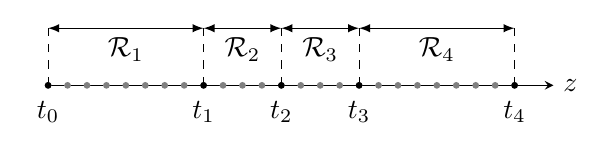
\begin{tikzpicture}
	\begin{axis}[width=8cm,height=4cm,xmin=0,xmax=6.5,xlabel=$z$,axis x line=middle,axis y line=none,xtick={0,2,3,4,6},xticklabels={$t_0$,$t_1$,$t_2$,$t_3$,$t_4$},xtick style={draw=none},every axis x label/.style={at=(current axis.right of origin),anchor=west},domain=0:6]
		\addplot[mark=*,mark size=1pt,only marks,color=gray] {0};
		\addplot[mark=*,mark size=1pt,only marks,color=black] coordinates{(0,0) (2,0) (3,0) (4,0) (6,0)};
		\draw[color=black,dashed] (0,0) -- (0,0.6);
		\draw[color=black,dashed] (2,0) -- (2,0.6);
		\draw[color=black,dashed] (3,0) -- (3,0.6);
		\draw[color=black,dashed] (4,0) -- (4,0.6);
		\draw[color=black,dashed] (6,0) -- (6,0.6);
		\draw[latex-latex] (0,0.6) -- (2,0.6) node[below,midway]{$\mathcal{R}_1$};
		\draw[latex-latex] (2,0.6) -- (3,0.6) node[below,midway]{$\mathcal{R}_2$};
		\draw[latex-latex] (3,0.6) -- (4,0.6) node[below,midway]{$\mathcal{R}_3$};
		\draw[latex-latex] (4,0.6) -- (6,0.6) node[below,midway]{$\mathcal{R}_4$};
	\end{axis}
\end{tikzpicture}

			}
			\caption{The decision thresholds are selected from fine-grained discrete energy levels instead of continuous space, and each decision region consists of at least one neighbor energy bins.}
			\label{fg:discrete_outputs}
		\end{figure}
		As shown in Fig.~\ref{fg:discrete_outputs}, by introducing an extra analog-to-digital conversion, we can group adjacent high-resolution energy bins to construct backscatter decision regions.
		Thus, problem \eqref{op:decision_threshold} can be recast as
		\begin{maxi!}
			{\scriptstyle{\boldsymbol{t} \in \mathcal{T}^{L+1}}}{I_{\text{B}}(x_{\mathcal{K}};\hat{x}_{\mathcal{K}})}{\label{op:decision_threshold_discrete}}{\label{ob:decision_threshold_discrete}}
			\addConstraint{\eqref{co:sequential_threshold},}
		\end{maxi!}
		which is solvable using existing rate-optimal sequential quantizer designs for \gls{dmtc}.
		To obtain global optimal solution, \cite{He2021} started from the quadrangle inequality and proposed a \gls{dp} method accelerated by the \gls{smawk} algorithm with computational complexity $\mathcal{O}\bigl(L^2(\mathrm{card}(\mathcal{T})-L)\bigr)$, while \cite{Nguyen2020a} started from the optimality condition for three neighbor thresholds and presented a traverse-then-bisect algorithm with complexity $\mathcal{O}\bigl(\mathrm{card}(\mathcal{T})L\log(\mathrm{card}(\mathcal{T})L)\bigr)$.
		In Section \ref{st:simulation_results}, both schemes will be compared with the \gls{ml} scheme \cite{Qian2019}
		\begin{equation}
			t_{l}^{\text{\gls{ml}}} = N \frac{\sigma_{l-1}^2 \sigma_{l}^2}{\sigma_{l-1}^2 - \sigma_{l}^2} \log \frac{\sigma_{l-1}^2}{\sigma_{l}^2}, \quad l \in \mathcal{L} \setminus \{L\},
			\label{eq:detection_threshold_ml}
		\end{equation}
		which is generally suboptimal for problem \eqref{op:decision_threshold} except when all nodes are with equiprobable inputs.
	\end{subsection}
\end{section}

\begin{section}{Simulation Results}
	In this section, we provide numerical results to evaluate the proposed input distribution, active beamforming, and backscatter decision designs for the considered RIScatter system.
	We assume the AP-user distance is \qty{10}{\meter} and at least one RIScatter nodes are randomly dropped in a disk centered at the user with radius $r$.
	% The \gls{ap} is with an average transmit power budget $P=\qty{36}{\dBm}$, all nodes employs $M$-\gls{qam} with amplitude scattering ratio $\alpha=0.5$, and the user is with average noise power $\sigma_v^2=\qty{-40}{\dBm}$.
	The \gls{ap} is with an average transmit power budget $P=\qty{36}{\dBm}$ and all nodes employs $M$-\gls{qam} with common amplitude scattering ratio $\alpha=0.5$.
	For all channels involved, we consider a distance-dependent path loss model
	\begin{equation}
		L(d) = L_0 \biggl(\frac{d_0}{d}\biggr)^\gamma,
	\end{equation}
	together with a Rician fading model
	\begin{equation}
		\boldsymbol{H} = \sqrt{\frac{\kappa}{1+\kappa}} \bar{\boldsymbol{H}} + \sqrt{\frac{1}{1+\kappa}} \tilde{\boldsymbol{H}},
	\end{equation}
	where $d$ is the transmission distance, $L_0=-\qty{30}{\dB}$ is the reference path loss at $d_0=\qty{1}{\meter}$, $\kappa$ is the Rician $K$-factor, $\bar{\boldsymbol{H}}$ is the deterministic line-of-sight component with unit-magnitude entries, and $\tilde{\boldsymbol{H}}$ is the Rayleigh fading component with standard \gls{iid} \gls{cscg} entries.
	We choose $\gamma_{\text{D}}=2.6$, $\gamma_{\text{F}}=2.4$, $\gamma_{\text{B}}=2$, and $\kappa_{\text{D}}=\kappa_{\text{F}}=\kappa_{\text{B}}=5$ for direct, forward and backward links.
	The finite decision threshold domain $\mathcal{T}$ is obtained by $b$-bit uniform discretization over the critical interval defined by the confidence bounds of edge hypotheses (i.e., lower bound of $\mathcal{H}_1$ and upper bound of $\mathcal{H}_L$) with confidence $1-\epsilon$, and we choose $b=9$ and $\epsilon=\num{e-3}$.
	All achievable rate points/regions are averaged over \num{e3} channel realizations.

	\begin{subsection}{Evaluation of Proposed Algorithms}
		\begin{subsubsection}{Initialization}
			To characterize each achievable rate region, we progressively obtain all boundary points by successively increasing the primary \gls{qos} $\rho$ and solving problem \eqref{op:weighted_sum_rate}.
			For $\rho=0$ where the backscatter link is prioritized, we initialize Algorithm \ref{al:input_distribution} and \ref{al:active_beamforming} by uniform input distribution and \gls{mrt} towards the sum cascaded channel $\sum_{k} \boldsymbol{h}_{\text{C},k}^\mathsf{H}$, respectively.
			At the following points, both algorithms are initialized by the final solutions at the previous point.
		\end{subsubsection}

		\begin{subsubsection}{Convergence}
			\begin{figure}[!t]
				\centering
				\resizebox{0.75\columnwidth}{!}{
					% This file was created by matlab2tikz.
%
%The latest updates can be retrieved from
%  http://www.mathworks.com/matlabcentral/fileexchange/22022-matlab2tikz-matlab2tikz
%where you can also make suggestions and rate matlab2tikz.
%
\definecolor{mycolor1}{rgb}{0.00000,0.44706,0.74118}%
\definecolor{mycolor2}{rgb}{0.85098,0.32549,0.09804}%
\definecolor{mycolor3}{rgb}{0.92941,0.69412,0.12549}%
%
\begin{tikzpicture}

\begin{axis}[%
width=4.053in,
height=0.919in,
at={(0.68in,2.887in)},
scale only axis,
xmin=0,
xmax=120,
ymin=0.113244880454575,
ymax=0.116102304831398,
axis background/.style={fill=white},
xmajorgrids,
ymajorgrids,
legend style={at={(0.97,0.03)}, anchor=south east, legend cell align=left, align=left, draw=white!15!black},
title style={font=\Large},
label style={font=\Large},
ticklabel style={font=\large},
legend style={font=\large},
yticklabel=\pgfkeys{/pgf/number format/.cd,fixed,precision=3}\pgfmathprintnumber{\tick}
]
\addplot [color=mycolor1, line width=2.0pt, mark=o, mark options={solid, mycolor1}]
  table[row sep=crcr]{%
0	0.113244880454575\\
10	0.114358992707155\\
20	0.114956255981364\\
30	0.115310191711237\\
40	0.115536251457935\\
50	0.11568965371294\\
60	0.115799285291346\\
70	0.115881218617581\\
80	0.115944814587431\\
90	0.115995739004593\\
100	0.116037546854275\\
110	0.116072549598378\\
120	0.116102304831398\\
};
\addlegendentry{KKT}

\end{axis}

\begin{axis}[%
width=4.053in,
height=0.919in,
at={(0.68in,1.67in)},
scale only axis,
xmin=0,
xmax=14,
ymin=0.116354276985174,
ymax=0.157617738080098,
ylabel style={font=\color{white!15!black}},
ylabel={Weighed Sum-Rate},
axis background/.style={fill=white},
xmajorgrids,
ymajorgrids,
legend style={at={(0.97,0.03)}, anchor=south east, legend cell align=left, align=left, draw=white!15!black},
title style={font=\Large},
label style={font=\Large},
ticklabel style={font=\large},
legend style={font=\large},
yticklabel=\pgfkeys{/pgf/number format/.cd,fixed,precision=3}\pgfmathprintnumber{\tick}
]
\addplot [color=mycolor2, dashed, line width=2.0pt, mark=+, mark options={solid, mycolor2}]
  table[row sep=crcr]{%
0	0.116354276985174\\
1	0.134986216301261\\
2	0.137045463164113\\
3	0.14221149883543\\
4	0.143513293823474\\
5	0.148182976472748\\
6	0.148354041018766\\
7	0.150388146565952\\
8	0.151376635136393\\
9	0.15160915733737\\
10	0.15291935995385\\
11	0.156743857286177\\
12	0.157617738080098\\
13	0.157617738080098\\
};
\addlegendentry{PGD}

\end{axis}

\begin{axis}[%
width=4.053in,
height=0.919in,
at={(0.68in,0.453in)},
scale only axis,
xmin=0,
xmax=8,
xlabel style={font=\color{white!15!black}},
xlabel={Number of Iterations},
ymin=0,
ymax=0.765555326497281,
axis background/.style={fill=white},
xmajorgrids,
ymajorgrids,
legend style={at={(0.97,0.03)}, anchor=south east, legend cell align=left, align=left, draw=white!15!black},
title style={font=\Large},
label style={font=\Large},
ticklabel style={font=\large},
legend style={font=\large},
yticklabel=\pgfkeys{/pgf/number format/.cd,fixed,precision=3}\pgfmathprintnumber{\tick}
]
\addplot [color=mycolor3, dotted, line width=2.0pt, mark=square, mark options={solid, mycolor3}]
  table[row sep=crcr]{%
0	0.113244880454575\\
1	0.159820508450486\\
2	0.271161604498627\\
3	0.403558255259651\\
4	0.594995557319089\\
5	0.748644776092643\\
6	0.764477923292286\\
7	0.765555325740019\\
8	0.765555326497281\\
};
\addlegendentry{BCD}

\end{axis}
\end{tikzpicture}%
				}
				\caption{Typical convergence curves at $\rho=0$ for $Q=4$, $K=8$, $M=2$, $N=20$, $\sigma_v^2=\qty{-40}{\dBm}$ and $r=\qty{2}{\meter}$.}
				\label{fg:wsr_convergence}
			\end{figure}

			In Fig.~\ref{fg:wsr_convergence}, we plot the weighted sum of primary and total backscatter rates at $\rho=0$ for \gls{kkt}, \gls{pgd} and \gls{bcd} algorithms on the first call.
			For $K=8$ and $M=2$, Algorithm \ref{al:input_distribution} typically takes around \num{100} fast iterations by \eqref{eq:input_kkt_solution} to converge to the \gls{kkt} input distribution.
			For $Q=4$, around \num{10} iterations are required for Algorithm \ref{al:active_beamforming} to converge, where the gradient is computed by \eqref{eq:weighted_sum_mutual_information_gradient} and the step size is refined by \gls{bls}.
			Overall, the \gls{bcd} algorithm initially requires at most \num{5} iterations to converge.
			At the following points (not presented here), the convergence of all three algorithms are much faster thanks to the progressive initialization.
			Hence, we conclude the proposed algorithms have good convergence performances.
		\end{subsubsection}
	\end{subsection}

	\begin{subsection}{Comparison of Scattering Applications}
		On top of the setup in Fig.~\ref{fg:riscatter_network}, we consider RIScatter and the following benchmark applications:
		\begin{itemize}
			\item \emph{Legacy:} Conventional active transmission without antenna mode scattering, $\alpha=0$.
			\item \emph{\gls{bbc}:} The primary symbol becomes deterministic $s[n]=1$ and the receive signal at each primary block is
			\begin{equation}
				y^{\text{\gls{bbc}}}[n] = \Bigl(\boldsymbol{h}_{\text{D}}^\mathsf{H} + \sum_{k} \alpha_k \boldsymbol{h}_{\text{C},k}^\mathsf{H} x_k\Bigr) \boldsymbol{w} + v[n],
			\end{equation}
			which follows non-zero mean complex Gaussian distribution $\mathcal{CN}\bigl((\boldsymbol{h}_{\text{D}}^\mathsf{H} + \sum_{k} \alpha_k \boldsymbol{h}_{\text{C},k}^\mathsf{H} x_{m_k}) \boldsymbol{w},\sigma_v^2\bigr)$ under hypothesis $\mathcal{H}_{m_{\mathcal{K}}}$.
			The corresponding \gls{pdf} of accumulated receive energy over $N$ primary blocks is
			\begin{equation}
				f^{\text{\gls{bbc}}}(z|\mathcal{H}_{m_{\mathcal{K}}}) = \frac{(z-\mu_{m_{\mathcal{K}}}^{\text{\gls{bbc}}})^{N-1} \exp \bigl(-(z-\mu_{m_{\mathcal{K}}}^{\text{\gls{bbc}}})/\sigma_v^2 \bigr)}{\sigma_v^{2N} (N-1)!},
				\label{eq:energy_distribution_bbc}
			\end{equation}
			where $\mu_{m_{\mathcal{K}}}^{\text{\gls{bbc}}} \triangleq N \bigl\lvert \bigl(\boldsymbol{h}_{\text{D}}^\mathsf{H} + \sum_{k} \alpha_k \boldsymbol{h}_{\text{C},k}^\mathsf{H} x_{m_k}\bigr) \boldsymbol{w} \bigr\rvert^2$.
			The \gls{ml} decision threshold is derived as, $\forall l \in \mathcal{L} \setminus \{L\}$,
			\begin{equation}
				t_l^{\text{\gls{bbc}}} = \frac{\mu_{l-1}^{\text{\gls{bbc}}} \exp \bigl((\mu_{l-1}^{\text{\gls{bbc}}}-\mu_{l}^{\text{\gls{bbc}}})/\sigma_v^2 (N-1)\bigr) - \mu_{l}^{\text{\gls{bbc}}}}{\exp \bigl((\mu_{l-1}^{\text{\gls{bbc}}}-\mu_{l}^{\text{\gls{bbc}}})/\sigma_v^2 (N-1)\bigr) - 1}.
				\label{eq:detection_threshold_ml_bbc}
			\end{equation}
			\item \emph{\gls{ambc}:} The user decodes both links independently and semi-coherently by treating the other as interference.
			Hence, the primary achievable rate is approximately\footnote{To provide a preliminary benchmark, we consider the (correlated) scattered signal from finite-input backscatter sources as independent interference from Gaussian sources during primary decoding \cite{Long2020a}.}
			\begin{equation}
				I_{\text{P}}^{\text{\gls{ambc}}}(s;y) \approx \log \Bigl(1 + \frac{\lvert\boldsymbol{h}_{\text{D}}^\mathsf{H}\boldsymbol{w}\rvert^2}{\sum_{k}\lvert \alpha_k \boldsymbol{h}_{\text{C},k}^\mathsf{H} \boldsymbol{w}\rvert^2+\sigma_v^2}\Bigr),
			\end{equation}
			while the total backscatter rate follows \eqref{eq:backscatter_mutual_information} with uniform input distribution.
			\item \emph{\gls{sr}:} For a sufficiently large $N$, the average primary rate under semi-coherent detection asymptotically approaches \eqref{eq:primary_mutual_information} with uniform input distribution \cite{Long2020a}.
			When $s[n]$ is successfully decoded and the direct interference $\boldsymbol{h}_{\text{D}}^\mathsf{H} \boldsymbol{w} s[n]$ is perfectly cancelled, the intermediate signal is
			\begin{equation}
				\hat{y}^{\text{\gls{sr}}}[n] = \sum_{k} \alpha_k \boldsymbol{h}_{\text{C},k}^\mathsf{H} x_k \boldsymbol{w} s[n] + v[n],
				\label{eq:intermediate_signal}
			\end{equation}
			which only involves noise uncertainty under hypothesis $\mathcal{H}_{m_{\mathcal{K}}}$.
			During backscatter detection, the primary symbols $s[1],\ldots,s[N]$ function as a spreading code and the receiver performs \gls{mrc} on $\hat{y}^{\text{\gls{sr}}}[n]$ over $N$ primary blocks.
			This essentially formulates a discrete-input continuous-output memoryless channel and the total backscatter achievable rate is maximized with equiprobable inputs as \cite{Ng2006}
			\begin{equation}
				I_{\text{B}}(x_{\mathcal{K}};\hat{y}^{\text{\gls{sr}}}) = K \log M - \frac{\iota}{M^K},
			\end{equation}
			where $\iota \triangleq \sum_{m_{\mathcal{K}}} \mathbb{E}_{\hat{v}} \log \sum_{m_{\mathcal{K}}'} \exp ( - {\lvert x_{m_{\mathcal{K}}} - x_{m_{\mathcal{K}}'} + \hat{v} \rvert^2}/{2 \sigma^2} )$ and $\hat{v} \sim \mathcal{CN}(0,\sigma_v^2/N)$.
			% For a sufficiently large $N$, $\iota$ is negligible and the total backscatter rate approaches $K \log M$.
			\item \emph{\gls{ris}:} Since the backscatter symbol tuple $x_{\mathcal{K}}$ is deterministic, the total backscatter rate is zero and the primary achievable rate becomes a special case of \eqref{eq:primary_mutual_information}
			\begin{equation}
				I_{\text{P}}^{\text{\gls{ris}}}(s;y|x_{\mathcal{K}}) = I_{\text{P}}(s;y|x_{m_{\mathcal{K}}^{\star}}) = \log \Bigl(1 + \frac{\lvert \boldsymbol{h}_{\text{E}}^\mathsf{H}(x_{m_{\mathcal{K}}^{\star}}) \boldsymbol{w} \rvert^2}{\sigma_v^2}\Bigr),
			\end{equation}
			where $m_{\mathcal{K}}^{\star} = \arg \max_{m_{\mathcal{K}}} I_{\text{P}}(s;y|x_{m_{\mathcal{K}}})$.
		\end{itemize}
		\begin{figure}[!t]
			\centering
			\resizebox{0.65\columnwidth}{!}{
				% This file was created by matlab2tikz.
%
%The latest updates can be retrieved from
%  http://www.mathworks.com/matlabcentral/fileexchange/22022-matlab2tikz-matlab2tikz
%where you can also make suggestions and rate matlab2tikz.
%
\definecolor{mycolor1}{rgb}{0.30100,0.74500,0.93300}%
\definecolor{mycolor2}{rgb}{0.46600,0.67400,0.18800}%
\definecolor{mycolor3}{rgb}{0.49400,0.18400,0.55600}%
\definecolor{mycolor4}{rgb}{0.92900,0.69400,0.12500}%
\definecolor{mycolor5}{rgb}{0.85000,0.32500,0.09800}%
\definecolor{mycolor6}{rgb}{0.00000,0.44700,0.74100}%
%
\begin{tikzpicture}

\begin{axis}[%
width=4.079in,
height=1.587in,
at={(0.684in,0.361in)},
scale only axis,
xmin=0,
xmax=6.5227548374066,
xlabel style={font=\color{white!15!black}},
xlabel={Primary Rate [bits/s/Hz]},
ymin=0,
ymax=2,
ylabel style={font=\color{white!15!black}},
ylabel={Backscatter\\Rate [bits/BB]},
axis background/.style={fill=white},
xmajorgrids,
ymajorgrids,
legend style={at={(0.03,0.03)}, anchor=south west, legend cell align=left, align=left, draw=white!15!black},
align=center,
title style={font=\LARGE},
label style={font=\LARGE},
ticklabel style={font=\Large},
legend style={font=\Large},
reverse legend,
every axis plot/.append style={line width=2pt}
]
\addplot [color=mycolor1, line width=2.0pt, mark=triangle, mark options={solid, rotate=180, mycolor1}]
  table[row sep=crcr]{%
6.33724402501803	1.39764296268229\\
0	1.39764296268229\\
0	0\\
6.52275483678685	0\\
6.52275483678685	2.37312052924553e-08\\
6.38739454470992	1.3235811846854\\
6.35422040211439	1.38916612409166\\
6.34857862205488	1.39386686170527\\
6.3445353675389	1.39608085009443\\
6.34291602910554	1.3966977322109\\
6.34149846039129	1.39711118534274\\
6.34024731759122	1.39737797077851\\
6.3391350240222	1.3975379071887\\
6.33862394227692	1.39758701988787\\
6.33813974610465	1.39761939115801\\
6.33795313341839	1.39762818964178\\
6.33777036860279	1.39763482338317\\
6.3375913342378	1.3976394187338\\
6.33741590881855	1.39764209463684\\
6.33724402501803	1.39764296268229\\
};
\addlegendentry{RIScatter}

\addplot[only marks, mark=triangle, mark options={}, mark size=2.3570pt, draw=mycolor2] table[row sep=crcr]{%
x	y\\
6.5227548374066	0\\
};
\addlegendentry{RIS}

\addplot[only marks, mark=+, mark options={}, mark size=3.5355pt, draw=mycolor3] table[row sep=crcr]{%
x	y\\
6.34321982467796	2\\
};
\addlegendentry{SR}

\addplot[only marks, mark=x, mark options={}, mark size=3.5355pt, draw=mycolor4] table[row sep=crcr]{%
x	y\\
5.90778796357092	1.34857377961699\\
};
\addlegendentry{AmBC}

\addplot[only marks, mark=square, mark options={}, mark size=2.5000pt, draw=mycolor5] table[row sep=crcr]{%
x	y\\
0	1.99999999999997\\
};
\addlegendentry{BBC}

\addplot[only marks, mark=o, mark options={}, mark size=2.7386pt, draw=mycolor6] table[row sep=crcr]{%
x	y\\
6.34314881160129	0\\
};
\addlegendentry{Legacy}

\end{axis}
\end{tikzpicture}%
			}
			\caption{Typical achievable rate region/points of scattering applications for $Q=1$, $K=1$, $M=4$, $N=e3$, $\sigma_v^2=\qty{-40}{\dBm}$ and $r=\qty{2}{\meter}$.}
			\label{fg:region_comparison}
		\end{figure}

		Fig.~\ref{fg:region_comparison} compares the typical achievable rate region/points of RIScatter and above.
		\emph{First,} we observe both \gls{bbc} and \gls{sr} almost ensure noise-free backscatter transmission when the spreading factor $N$ is sufficiently large.
		For \gls{bbc} with coherent energy detection, the conditional \gls{pdf} of accumulated receive energy \eqref{eq:energy_distribution_bbc} is more skewed at a large $N$, such that the equivalent \gls{dmtmac} \eqref{eq:dmtmac} has lower error probabilities.
		For \gls{sic}-based \gls{sr}, the effective backscatter \gls{snr} is increased by $N$ times and the penalty term $\iota$ becomes insignificant.
		However, the primary rate is only maintained at a very large spreading factor, which significantly constrains the backscatter \emph{throughput}.
		\emph{Second,} the average primary rate slightly increases/decreases in the presence of a \gls{ambc}/\gls{ris} node, and the multipath benefit of \gls{sr} is unobvious.
		This is because the cascaded channel can be orders of magnitude weaker than the direct channel due to the double fading effect.
		\gls{ris} always ensures constructive superposition of direct and scattered components, while \gls{sr} only creates a quasi-static rich-scattering environment that \emph{stochastically} enhances the average primary rate.
		When $N$ is moderate, the randomly scattered signals should be modelled as primary interference rather than multipath components, and the \gls{sr} point will move towards the \gls{ambc} point.
		\emph{Third,} RIScatter enables a flexible primary-backscatter tradeoff with adaptive input distribution design.
		In terms of maximum primary achievable rate, RIScatter coincides with \gls{ris} and outperforms the others with passive beamforming provided by deterministic reflection pattern.
		On the other hand, for a large $N$, the maximum backscatter achievable rate of RIScatter is higher than \gls{ambc} but lower than \gls{bbc} and \gls{sr}.
		This is because both RIScatter and \gls{ambc} (resp. \gls{bbc} and \gls{sr}) employ semi-coherent (resp. coherent) energy detection, while RIScatter with adaptive channel coding can achieve higher backscatter rate than \gls{ambc} with equiprobable inputs.
		Importantly, such a practical RIScatter detection is feasible for arbitrary spreading factor, which unleashes the potential of fast-switching nodes.
		% , and using a fast-switching node with smaller $N$ can increase the backscatter throughput per unit time while preserving the dynamic passive beamforming gain on the primary link.
	\end{subsection}

	\begin{subsection}{Input Distribution under Different \gls{qos}}
		\begin{figure}[!t]
			\centering
			\resizebox{0.65\columnwidth}{!}{
				% This file was created by matlab2tikz.
%
%The latest updates can be retrieved from
%  http://www.mathworks.com/matlabcentral/fileexchange/22022-matlab2tikz-matlab2tikz
%where you can also make suggestions and rate matlab2tikz.
%
\definecolor{mycolor1}{rgb}{0.00000,0.44706,0.74118}%
\definecolor{mycolor2}{rgb}{0.85098,0.32549,0.09804}%
\definecolor{mycolor3}{rgb}{0.92941,0.69412,0.12549}%
\definecolor{mycolor4}{rgb}{0.49412,0.18431,0.55686}%
%
\begin{tikzpicture}

\begin{axis}[%
width=4.079in,
height=3.432in,
at={(0.684in,0.463in)},
scale only axis,
xmin=1,
xmax=4,
xtick={1, 2, 3, 4},
xlabel style={font=\color{white!15!black}},
xlabel={Reflection State},
ymin=0,
ymax=1,
ytick={  0, 0.2, 0.4, 0.6, 0.8,   1},
ylabel style={font=\color{white!15!black}},
ylabel={Probability Distribution},
axis background/.style={fill=white},
xmajorgrids,
ymajorgrids,
legend style={legend cell align=left, align=left, draw=white!15!black},
title style={font=\LARGE},
label style={font=\LARGE},
ticklabel style={font=\Large},
legend style={font=\Large}
]
\addplot [color=mycolor1, line width=2.0pt, mark=o, mark options={solid, mycolor1}]
  table[row sep=crcr]{%
1	5.58936301883394e-08\\
2	0.494967846198009\\
3	0.505032051077508\\
4	4.68308531955441e-08\\
};
\addlegendentry{$\rho =0$}

\addplot [color=mycolor2, dashed, line width=2.0pt, mark=+, mark options={solid, mycolor2}]
  table[row sep=crcr]{%
1	3.50493170830856e-09\\
2	0.586489834632108\\
3	0.413510159250847\\
4	2.6121135277758e-09\\
};
\addlegendentry{$\rho =0.1$}

\addplot [color=mycolor3, dotted, line width=2.0pt, mark=square, mark options={solid, mycolor3}]
  table[row sep=crcr]{%
1	1.54239700394178e-10\\
2	0.770075793479604\\
3	0.229924206275344\\
4	9.08124388871134e-11\\
};
\addlegendentry{$\rho =0.25$}

\addplot [color=mycolor4, dashdotted, line width=2.0pt, mark=x, mark options={solid, mycolor4}]
  table[row sep=crcr]{%
1	1.62167297049731e-12\\
2	0.999999185020827\\
3	8.14977502370884e-07\\
4	4.9209962545264e-14\\
};
\addlegendentry{$\rho =1$}

\end{axis}
\end{tikzpicture}%
			}
			\caption{Typical RIScatter reflection state distribution at different $\rho$ for $Q=1$, $K=1$, $M=4$, $N=20$, $\sigma_v^2=\qty{-40}{\dBm}$ and $r=\qty{2}{\meter}$.}
			\label{fg:distribution_weights}
		\end{figure}
		The objective of this study is to demonstrate RIScatter nodes can leverage \gls{csi}- and \gls{qos}-adaptive input distribution design to balance backscatter modulation and passive beamforming.
		For one RIScatter node with $M=4$, we evaluate the \gls{kkt} input distribution\footnote{Since problem \eqref{op:input_distribution} is convex when $K=1$, the \gls{kkt} solution is always global optimal in this case.} at different primary \gls{qos} and present the result in Fig.~\ref{fg:distribution_weights}.
		At $\rho=0$ where the backscatter performance is prioritized, the optimal input distribution is zero on two states and nearly uniform on the other two.
		This is because, due to the weak scattered signal, the conditional energy \gls{pdf} under different hypotheses can be closely spaced as illustrated in Fig.~\ref{fg:energy_distribution}.
		In such cases, the extreme states producing the lowest/highest energy are always assigned with non-zero probability, while the middle ones may not provide enough energy difference and thus end up unused.
		At $\rho=1$ where the primary performance is prioritized, the optimal input distribution is \num{1} at the state that maximizes the primary \gls{snr} and \num{0} at the others.
		That is, the reflection pattern becomes deterministic and the RIScatter node boils down to a discrete \gls{ris} element.
		Increasing $\rho$ from \num{0} to \num{1} provides a smooth transition from backscatter modulation to passive beamforming, which suggests RIScatter unifies \gls{bc} and \gls{ris} from a probabilistic perspective.
	\end{subsection}

	\begin{subsection}{Rate Region by Different Schemes}
		\begin{figure}[!t]
			\centering
			\subfloat[Input Distribution, $Q=1$\label{fg:region_distribution}]{
				\resizebox{0.6\columnwidth}{!}{
					% This file was created by matlab2tikz.
%
%The latest updates can be retrieved from
%  http://www.mathworks.com/matlabcentral/fileexchange/22022-matlab2tikz-matlab2tikz
%where you can also make suggestions and rate matlab2tikz.
%
\definecolor{mycolor1}{rgb}{0.00000,0.44706,0.74118}%
\definecolor{mycolor2}{rgb}{0.85098,0.32549,0.09804}%
\definecolor{mycolor3}{rgb}{0.92941,0.69412,0.12549}%
\definecolor{mycolor4}{rgb}{0.49412,0.18431,0.55686}%
\definecolor{mycolor5}{rgb}{0.46667,0.67451,0.18824}%
\definecolor{mycolor6}{rgb}{0.30196,0.74510,0.93333}%
\definecolor{mycolor7}{rgb}{0.63529,0.07843,0.18431}%
%
\begin{tikzpicture}

	\begin{axis}[%
			width=4.014in,
			height=3.389in,
			at={(0.673in,0.457in)},
			scale only axis,
			xmin=6,xmax=6.55,
			xtick={6,6.1,6.2,6.3,6.4,6.5},
			xlabel style={font=\color{white!15!black}},
			xlabel={Primary Rate [bits/s/Hz]},
			ymin=0,
			ymax=0.258249123037508,
			ylabel style={font=\color{white!15!black}},
			ylabel={Total Backscatter Rate [bits/BB]},
			axis background/.style={fill=white},
			xmajorgrids,
			ymajorgrids,
			legend style={at={(0.03,0.03)}, anchor=south west, legend cell align=left, align=left, draw=white!15!black},
			title style={font=\LARGE},
			label style={font=\LARGE},
			ticklabel style={font=\Large},
			legend style={font=\Large},
			scaled y ticks=false,
			y tick label style={/pgf/number format/.cd, fixed, precision=2}
		]
		\addplot [color=mycolor1, line width=2.0pt, mark=o, mark options={solid, mycolor1}]
		table[row sep=crcr]{%
				6.32146282014783	0.135298434401071\\
				0	0.135298434401071\\
				0	0\\
				6.54733712865232	0\\
				6.54517433822466	0.00774868535999835\\
				6.50756053444898	0.0675347647522537\\
				6.47890595069851	0.0908447067770361\\
				6.4405754582915	0.111410986078138\\
				6.41906097335963	0.119575938134352\\
				6.39711048749103	0.125961202920399\\
				6.375794485304	0.130496464040102\\
				6.35566511647813	0.13338720543392\\
				6.34622485273269	0.134291841616495\\
				6.33755099968818	0.134871348283307\\
				6.3341180598223	0.135032749667558\\
				6.33078786275436	0.135153660987559\\
				6.3275979313462	0.135235752926375\\
				6.32449832330173	0.135283108344685\\
				6.32146282014783	0.135298434401071\\
			};
		\addlegendentry{Exhaustion}

		\addplot [color=mycolor2, dashed, line width=2.0pt, mark=+, mark options={solid, mycolor2}]
		table[row sep=crcr]{%
				6.32141918409994	0.135302553290759\\
				0	0.135302553290759\\
				0	0\\
				6.54617494292906	0\\
				6.54617494292906	5.35569540967736e-08\\
				6.54395549026001	0.00794380155151132\\
				6.50571395400754	0.0685517046188535\\
				6.47725030932065	0.0915613607821624\\
				6.43904818034038	0.111868185202614\\
				6.41734122875771	0.119998466631658\\
				6.39569411793482	0.126224654256524\\
				6.37478946505091	0.130639435722587\\
				6.35513830914346	0.133439138952041\\
				6.34596989012747	0.134312547131226\\
				6.33728397409874	0.134887798900337\\
				6.33394436296369	0.135043581861458\\
				6.33067909442514	0.135160647084426\\
				6.32748262520049	0.135241405287329\\
				6.32435855863608	0.135287987095764\\
				6.32141918409994	0.135302553290759\\
			};
		\addlegendentry{KKT}

		\addplot [color=mycolor3, dotted, line width=2.0pt, mark=square, mark options={solid, mycolor3}]
		table[row sep=crcr]{%
				6.33038216910371	0.258249123037508\\
				0	0.258249123037508\\
				0	0\\
				6.54733712865225	0\\
				6.54733712865225	9.63577398919082e-15\\
				6.53818045939347	0.0325698770891707\\
				6.43706862579333	0.205987678214288\\
				6.40319420024859	0.234129375981137\\
				6.37756789518431	0.24814619770397\\
				6.36712369262437	0.252123967734036\\
				6.35793773244948	0.25480261208027\\
				6.3498258540104	0.256532319837123\\
				6.34261469311561	0.257569015164329\\
				6.33930342588844	0.257887218672394\\
				6.33616929824435	0.258096765396561\\
				6.33496269926005	0.258153654718521\\
				6.33378166469514	0.258196523198478\\
				6.33262379024928	0.258226244645555\\
				6.33149125428708	0.258243521141676\\
				6.33038216910371	0.258249123037508\\
			};
		\addlegendentry{Cooperation}

		\addplot [color=mycolor4, dashdotted, line width=2.0pt, mark=x, mark options={solid, mycolor4}]
		table[row sep=crcr]{%
				6.3353047399281	0.132538456219543\\
				0	0.132538456219543\\
				0	0\\
				6.54733712865224	0\\
				6.54733712865224	4.9616544470467e-15\\
				6.53883907987144	0.0173736087216158\\
				6.44100451648281	0.104073934077473\\
				6.40767165852713	0.118546491406672\\
				6.38231104047054	0.126127571777712\\
				6.37194304642766	0.128392528291276\\
				6.36281278709048	0.129987574291472\\
				6.35472791571861	0.131088141723972\\
				6.34753142631954	0.131822608691493\\
				6.34422575990388	0.13208245385162\\
				6.34109503581159	0.132282820185509\\
				6.33988891868859	0.132348288736295\\
				6.33870564827907	0.132406206639739\\
				6.33754869585191	0.132457094231239\\
				6.33641540465384	0.13250082882571\\
				6.3353047399281	0.132538456219543\\
			};
		\addlegendentry{Marginalization}

		\addplot [color=mycolor5, line width=2.0pt, mark=triangle, mark options={solid, mycolor5}]
		table[row sep=crcr]{%
				6.33515135931876	0.0104508384451561\\
				0	0.0104508384451561\\
				0	0\\
				6.54733712865225	0\\
				6.54733712865225	9.41351914512674e-17\\
				6.54566316113138	0.0018911689220282\\
				6.50449357170924	0.00614593506985847\\
				6.47104644280986	0.00857077717475668\\
				6.33515135931876	0.0104508384451561\\
			};
		\addlegendentry{Decomposition}

		\addplot [color=mycolor6, dashed, line width=2.0pt, mark=triangle, mark options={solid, rotate=180, mycolor6}]
		table[row sep=crcr]{%
				6.51905860474812	0.040829341410189\\
				0	0.040829341410189\\
				0	0\\
				6.5473371278862	0\\
				6.5473371278862	1.13550059120926e-09\\
				6.54539615692803	0.00510452797145521\\
				6.51905860474812	0.040829341410189\\
			};
		\addlegendentry{Randomization}

		\addplot [color=mycolor7, dotted, line width=2.0pt, mark=triangle, mark options={solid, rotate=270, mycolor7}]
		table[row sep=crcr]{%
				6.34050352716188	0.131452428942456\\
				6.34050352716188	0.131452428942456\\
				6.34050352716188	0.131452428942456\\
				6.34050352716188	0.131452428942456\\
				6.34050352716188	0.131452428942456\\
				0	0.131452428942456\\
				0	0\\
				6.34050352716188	0\\
				6.34050352716188	0.131452428942456\\
			};
		\addlegendentry{Equiprobable}

	\end{axis}

	\begin{axis}[%
			width=1.036in,
			height=1.039in,
			at={(1.543in,2.588in)},
			scale only axis,
			separate axis lines,
			every outer x axis line/.append style={black},
			every x tick label/.append style={font=\color{black}},
			every x tick/.append style={black},
			xmin=6.324,
			xmax=6.36,
			every outer y axis line/.append style={black},
			every y tick label/.append style={font=\color{black}},
			every y tick/.append style={black},
			ymin=0.129114533984272,
			ymax=0.137036286224687,
			axis background/.style={fill=white!90!black},
			xmajorgrids,
			ymajorgrids,
			title style={font=\LARGE},
			label style={font=\LARGE},
			ticklabel style={font=\Large},
			legend style={font=\Large},
			scaled y ticks=false,
			y tick label style={/pgf/number format/.cd, fixed, precision=3}
		]
		\addplot [color=mycolor1, line width=2.0pt, mark=o, mark options={solid, mycolor1}, forget plot]
		table[row sep=crcr]{%
				6.32146282014783	0.135298434401071\\
				0	0.135298434401071\\
				0	0\\
				6.54733712865232	0\\
				6.54517433822466	0.00774868535999835\\
				6.50756053444898	0.0675347647522537\\
				6.47890595069851	0.0908447067770361\\
				6.4405754582915	0.111410986078138\\
				6.41906097335963	0.119575938134352\\
				6.39711048749103	0.125961202920399\\
				6.375794485304	0.130496464040102\\
				6.35566511647813	0.13338720543392\\
				6.34622485273269	0.134291841616495\\
				6.33755099968818	0.134871348283307\\
				6.3341180598223	0.135032749667558\\
				6.33078786275436	0.135153660987559\\
				6.3275979313462	0.135235752926375\\
				6.32449832330173	0.135283108344685\\
				6.32146282014783	0.135298434401071\\
			};
		\addplot [color=mycolor2, dashed, line width=2.0pt, mark=+, mark options={solid, mycolor2}, forget plot]
		table[row sep=crcr]{%
				6.32141918409994	0.135302553290759\\
				0	0.135302553290759\\
				0	0\\
				6.54617494292906	0\\
				6.54617494292906	5.35569540967736e-08\\
				6.54395549026001	0.00794380155151132\\
				6.50571395400754	0.0685517046188535\\
				6.47725030932065	0.0915613607821624\\
				6.43904818034038	0.111868185202614\\
				6.41734122875771	0.119998466631658\\
				6.39569411793482	0.126224654256524\\
				6.37478946505091	0.130639435722587\\
				6.35513830914346	0.133439138952041\\
				6.34596989012747	0.134312547131226\\
				6.33728397409874	0.134887798900337\\
				6.33394436296369	0.135043581861458\\
				6.33067909442514	0.135160647084426\\
				6.32748262520049	0.135241405287329\\
				6.32435855863608	0.135287987095764\\
				6.32141918409994	0.135302553290759\\
			};
		\addplot [color=mycolor3, dotted, line width=2.0pt, mark=square, mark options={solid, mycolor3}, forget plot]
		table[row sep=crcr]{%
				6.33038216910371	0.258249123037508\\
				0	0.258249123037508\\
				0	0\\
				6.54733712865225	0\\
				6.54733712865225	9.63577398919082e-15\\
				6.53818045939347	0.0325698770891707\\
				6.43706862579333	0.205987678214288\\
				6.40319420024859	0.234129375981137\\
				6.37756789518431	0.24814619770397\\
				6.36712369262437	0.252123967734036\\
				6.35793773244948	0.25480261208027\\
				6.3498258540104	0.256532319837123\\
				6.34261469311561	0.257569015164329\\
				6.33930342588844	0.257887218672394\\
				6.33616929824435	0.258096765396561\\
				6.33496269926005	0.258153654718521\\
				6.33378166469514	0.258196523198478\\
				6.33262379024928	0.258226244645555\\
				6.33149125428708	0.258243521141676\\
				6.33038216910371	0.258249123037508\\
			};
		\addplot [color=mycolor4, dashdotted, line width=2.0pt, mark=x, mark options={solid, mycolor4}, forget plot]
		table[row sep=crcr]{%
				6.3353047399281	0.132538456219543\\
				0	0.132538456219543\\
				0	0\\
				6.54733712865224	0\\
				6.54733712865224	4.9616544470467e-15\\
				6.53883907987144	0.0173736087216158\\
				6.44100451648281	0.104073934077473\\
				6.40767165852713	0.118546491406672\\
				6.38231104047054	0.126127571777712\\
				6.37194304642766	0.128392528291276\\
				6.36281278709048	0.129987574291472\\
				6.35472791571861	0.131088141723972\\
				6.34753142631954	0.131822608691493\\
				6.34422575990388	0.13208245385162\\
				6.34109503581159	0.132282820185509\\
				6.33988891868859	0.132348288736295\\
				6.33870564827907	0.132406206639739\\
				6.33754869585191	0.132457094231239\\
				6.33641540465384	0.13250082882571\\
				6.3353047399281	0.132538456219543\\
			};
		\addplot [color=mycolor5, line width=2.0pt, mark=triangle, mark options={solid, mycolor5}, forget plot]
		table[row sep=crcr]{%
				6.33515135931876	0.0104508384451561\\
				0	0.0104508384451561\\
				0	0\\
				6.54733712865225	0\\
				6.54733712865225	9.41351914512674e-17\\
				6.54566316113138	0.0018911689220282\\
				6.50449357170924	0.00614593506985847\\
				6.47104644280986	0.00857077717475668\\
				6.33515135931876	0.0104508384451561\\
			};
		\addplot [color=mycolor6, dashed, line width=2.0pt, mark=triangle, mark options={solid, rotate=180, mycolor6}, forget plot]
		table[row sep=crcr]{%
				6.51905860474812	0.040829341410189\\
				0	0.040829341410189\\
				0	0\\
				6.5473371278862	0\\
				6.5473371278862	1.13550059120926e-09\\
				6.54539615692803	0.00510452797145521\\
				6.51905860474812	0.040829341410189\\
			};
		\addplot [color=mycolor7, dotted, line width=2.0pt, mark=triangle, mark options={solid, rotate=270, mycolor7}, forget plot]
		table[row sep=crcr]{%
				6.34050352716188	0.131452428942456\\
				6.34050352716188	0.131452428942456\\
				6.34050352716188	0.131452428942456\\
				6.34050352716188	0.131452428942456\\
				6.34050352716188	0.131452428942456\\
				0	0.131452428942456\\
				0	0\\
				6.34050352716188	0\\
				6.34050352716188	0.131452428942456\\
			};
	\end{axis}

	\draw[-latex] (8,6) -- (6.85,7.25);
	\draw (7.8,5.43) rectangle ++(0.4,0.4);
	% \begin{axis}[%
	% width=5.179in,
	% height=4.158in,
	% at={(0in,0in)},
	% scale only axis,
	% xmin=0,
	% xmax=1,
	% ymin=0,
	% ymax=1,
	% axis line style={draw=none},
	% ticks=none,
	% axis x line*=bottom,
	% axis y line*=left,
	% title style={font=\LARGE},
	% label style={font=\LARGE},
	% ticklabel style={font=\Large},
	% legend style={font=\Large},
	% scaled y ticks=false,
	% y tick label style={/pgf/number format/.cd, fixed, precision=2}
	% ]
	% \draw[line width=1.0pt, draw=black] (axis cs:314.88,205.4) rectangle (axis cs:324.72,215.275);
	% \addplot [color=black, line width=1.0pt, forget plot]
	%   table[row sep=crcr]{%
	% 0.65	0.545\\
	% 0.500032520325203	0.75003164556962\\
	% };
	% \end{axis}
\end{tikzpicture}%

				}
			}
			\\
			\subfloat[Active Beamforming, $Q=4$\label{fg:region_beamforming}]{
				\resizebox{0.48\columnwidth}{!}{
					% This file was created by matlab2tikz.
%
%The latest updates can be retrieved from
%  http://www.mathworks.com/matlabcentral/fileexchange/22022-matlab2tikz-matlab2tikz
%where you can also make suggestions and rate matlab2tikz.
%
\definecolor{mycolor1}{rgb}{0.00000,0.44706,0.74118}%
\definecolor{mycolor2}{rgb}{0.85098,0.32549,0.09804}%
\definecolor{mycolor3}{rgb}{0.92941,0.69412,0.12549}%
%
\begin{tikzpicture}

\begin{axis}[%
width=4.079in,
height=3.432in,
at={(0.684in,0.463in)},
scale only axis,
xmin=0,
xmax=8.92881892981245,
xlabel style={font=\color{white!15!black}},
xlabel={Primary Rate [bits/s/Hz]},
ymin=0,
ymax=1.01992845118215,
ylabel style={font=\color{white!15!black}},
ylabel={Total Backscatter Rate [bits/BSP]},
axis background/.style={fill=white},
xmajorgrids,
ymajorgrids,
legend style={at={(0.03,0.03)}, anchor=south west, legend cell align=left, align=left, draw=white!15!black},
title style={font=\LARGE},
label style={font=\LARGE},
ticklabel style={font=\Large},
legend style={font=\Large},
scaled y ticks=false,
y tick label style={/pgf/number format/.cd, fixed, precision=2}
]
\addplot [color=mycolor1, line width=2.0pt, mark=o, mark options={solid, mycolor1}]
  table[row sep=crcr]{%
2.63559055942685	1.01992845118215\\
0	1.01992845118215\\
0	0\\
8.92028810777469	0\\
8.92028810777469	7.26950318495981e-08\\
8.91696984927535	0.0120256859659793\\
8.86979129856964	0.0846609824712485\\
8.82706648243075	0.117827710281232\\
8.75538403864464	0.154759583100072\\
8.70577272900074	0.171967620624558\\
8.47551795626764	0.226240844139463\\
6.38790092654795	0.59728412002455\\
3.66989487852363	0.94782263264172\\
3.1151172710216	0.995313620027521\\
2.79370603017906	1.0157860492444\\
2.74174413489818	1.01794066244276\\
2.71082935981954	1.01875660510405\\
2.68480358491872	1.01933845340111\\
2.63559055942685	1.01992845118215\\
};
\addlegendentry{PGD}

\addplot [color=mycolor2, dashed, line width=2.0pt, mark=+, mark options={solid, mycolor2}]
  table[row sep=crcr]{%
8.55305414925037	0.190532539562689\\
0	0.190532539562689\\
0	0\\
8.92881892981245	0\\
8.92881892981245	7.23815480998908e-08\\
8.92547114392242	0.0120236300404424\\
8.87966496840328	0.082734254382408\\
8.83910110870482	0.114387488553325\\
8.77329734415381	0.147798783367702\\
8.72958480083147	0.163219336150511\\
8.68430801388451	0.17533602280299\\
8.6410296368303	0.183574065460131\\
8.60095734022126	0.188376215138858\\
8.58278096266478	0.189661072048591\\
8.56577521877358	0.190353222247642\\
8.55931861959876	0.190472547071125\\
8.55305414925037	0.190532539562689\\
};
\addlegendentry{E-MRT}

\addplot [color=mycolor3, dotted, line width=2.0pt, mark=square, mark options={solid, mycolor3}]
  table[row sep=crcr]{%
8.54072704683782	0.191124905617539\\
0	0.191124905617539\\
0	0\\
8.92324086962215	0\\
8.92324086962215	7.36615731319728e-08\\
8.92011492095492	0.011227990559007\\
8.87691781721755	0.0788657412116758\\
8.83801903306622	0.109947771916532\\
8.77351584785445	0.143741679932563\\
8.73017345209674	0.159761546419946\\
8.68512782973099	0.172648165205386\\
8.6413558120408	0.181843168450172\\
8.60126605785167	0.187534392844755\\
8.58280631164911	0.189267907476186\\
8.56565171116225	0.190398333642165\\
8.55911321271799	0.190698539653517\\
8.55270893661118	0.190918610365619\\
8.54656023056819	0.191073249951565\\
8.54072704683782	0.191124905617539\\
};
\addlegendentry{D-MRT}

\end{axis}
\end{tikzpicture}%
				}
			}
			\subfloat[Decision Threshold, $Q=4$\label{fg:region_threshold}]{
				\resizebox{0.48\columnwidth}{!}{
					% This file was created by matlab2tikz.
%
%The latest updates can be retrieved from
%  http://www.mathworks.com/matlabcentral/fileexchange/22022-matlab2tikz-matlab2tikz
%where you can also make suggestions and rate matlab2tikz.
%
\definecolor{mycolor1}{rgb}{0.00000,0.44706,0.74118}%
\definecolor{mycolor2}{rgb}{0.85098,0.32549,0.09804}%
\definecolor{mycolor3}{rgb}{0.92941,0.69412,0.12549}%
\definecolor{mycolor4}{rgb}{0.49412,0.18431,0.55686}%
%
\begin{tikzpicture}

\begin{axis}[%
width=4.079in,
height=3.432in,
at={(0.684in,0.463in)},
scale only axis,
xmin=0,
xmax=8.76636939072744,
xlabel style={font=\color{white!15!black}},
xlabel={Primary Rate [bits/s/Hz]},
ymin=0,
ymax=0.712697053053165,
ylabel style={font=\color{white!15!black}},
ylabel={Total Backscatter Rate [bits/BSP]},
axis background/.style={fill=white},
xmajorgrids,
ymajorgrids,
legend style={at={(0.03,0.03)}, anchor=south west, legend cell align=left, align=left, draw=white!15!black},
title style={font=\LARGE},
label style={font=\LARGE},
ticklabel style={font=\Large},
legend style={font=\Large},
scaled y ticks=false,
y tick label style={/pgf/number format/.cd, fixed, precision=2}
]
\addplot [color=mycolor1, line width=2.0pt, mark=o, mark options={solid, mycolor1}]
  table[row sep=crcr]{%
2.32222859252816	0.712697053053165\\
0	0.712697053053165\\
0	0\\
8.76507816041105	0\\
8.76507816041105	7.42576077476074e-08\\
8.76388944486998	0.00420831360409523\\
8.74129115690256	0.0384594322949282\\
8.72081490076816	0.0548306456131603\\
8.6878146390259	0.0723079112108233\\
8.66572491150263	0.0804472514182304\\
8.63711211771591	0.0885825772177961\\
8.23901357242778	0.160420705216473\\
6.19582895638924	0.411214346326543\\
4.58583051565943	0.556309639607008\\
3.07691766196375	0.668685163411535\\
2.63025777386073	0.701548780799618\\
2.49994402971108	0.70948668509458\\
2.32222859252816	0.712697053053165\\
};
\addlegendentry{DP}

\addplot [color=mycolor2, dashed, line width=2.0pt, mark=+, mark options={solid, mycolor2}]
  table[row sep=crcr]{%
2.32222859252816	0.712697053053165\\
0	0.712697053053165\\
0	0\\
8.76507816041105	0\\
8.76507816041105	7.42576077476074e-08\\
8.76388944486998	0.00420831360409523\\
8.74129115690256	0.0384594322949282\\
8.72081490076816	0.0548306456131603\\
8.6878146390259	0.0723079112108233\\
8.66572491150263	0.0804472514182304\\
8.63711211771591	0.0885825772177961\\
8.23901357242778	0.160420705216473\\
6.19582895638924	0.411214346326543\\
4.58583051565943	0.556309639607008\\
3.07691766196375	0.668685163411535\\
2.63025777386073	0.701548780799618\\
2.49994402971108	0.70948668509458\\
2.32222859252816	0.712697053053165\\
};
\addlegendentry{SMAWK}

\addplot [color=mycolor3, dotted, line width=2.0pt, mark=square, mark options={solid, mycolor3}]
  table[row sep=crcr]{%
2.51679051521506	0.644331294694737\\
0	0.644331294694737\\
0	0\\
8.76491911226082	0\\
8.76491911226082	7.06583390240895e-08\\
8.76375272574725	0.00396063293661604\\
8.74142330131568	0.0381540336636628\\
8.72073994737061	0.054754968593519\\
8.68613720274916	0.0730500803444379\\
8.66366878557346	0.0815125259259304\\
8.63467842070196	0.0898334130105359\\
8.29193515127934	0.150948580402326\\
6.78161791277737	0.336671277192313\\
5.3114678490953	0.468317078354024\\
3.36425249555738	0.601535498045008\\
2.88372997776731	0.633725328238547\\
2.7586935248779	0.641137533661162\\
2.51679051521506	0.644331294694737\\
};
\addlegendentry{Bisection}

\addplot [color=mycolor4, dashdotted, line width=2.0pt, mark=x, mark options={solid, mycolor4}]
  table[row sep=crcr]{%
8.00091115235288	0.120737258590871\\
0	0.120737258590871\\
0	0\\
8.76636939072744	0\\
8.76636939072744	5.98436739715304e-08\\
8.76536378078933	0.00346637119824424\\
8.74629248555552	0.0330578688028253\\
8.7291469202831	0.0469634405169363\\
8.69727210179649	0.0639091368226758\\
8.67468378185317	0.0727343500662612\\
8.64300653905165	0.0823137844993143\\
8.59920170605537	0.0920437613859666\\
8.53438868199787	0.101414886698637\\
8.48136877838668	0.106777102094185\\
8.39487654373549	0.112520073621344\\
8.34783395500726	0.114851667246842\\
8.28365800949728	0.11720403163147\\
8.20678284232304	0.119143339906688\\
8.12143574716189	0.120439352696928\\
8.00091115235288	0.120737258590871\\
};
\addlegendentry{ML}

\end{axis}
\end{tikzpicture}%
				}
			}
			\caption{
				Average primary-total-backscatter rate regions by different input distribution, active beamforming, and decision threshold schemes for $K=2$, $M=4$, $N=20$, $\sigma_v^2=\qty{-40}{\dBm}$ and $r=\qty{2}{\meter}$.
			}
		\end{figure}
		\begin{subsubsection}{Input Distribution}
			We compare these input distribution designs for problem \eqref{op:input_distribution}:
			\begin{itemize}
				\item \emph{Cooperation:} Joint nodes encoding using a $K$-dimensional probability array $P_{\mathcal{K}}(x_{m_{\mathcal{K}}})$ by Algorithm \ref{al:input_distribution};
				\item \emph{Exhaustion:} Exhaustive search over the $M$-dimensional probability simplex with resolution $\Delta p = \num{e-2}$;
				\item \emph{\gls{kkt}:} Numerical \gls{kkt} result evaluation by Algorithm \ref{al:input_distribution};
				\item \emph{Equiprobable:} Uniform input distribution for all nodes.
			\end{itemize}
			For dispersed nodes, joint encoding is inapplicable and we consider these independent input distribution recovery methods (from the joint probability array):
			\begin{itemize}
				\item \emph{Marginalization:} Marginal probability distributions;
				\item \emph{Decomposition:} Normalized rank-\num{1} \gls{cp} decomposition tensors by \texttt{Tensor Toolbox} \cite{Bader2022};
				\item \emph{Randomization:} Gaussian randomization with the guidance of correlation matrix \cite{Calvo2010}.
				% guided by correlation matrix \cite{Calvo2010}.
			\end{itemize}

			Fig.~\subref*{fg:region_distribution} shows the average achievable rate regions for those designs.
			We observe \emph{Cooperation} provides the outer bound since joint encoding is always beneficial.
			The \emph{average} rate performance of \emph{Exhaustion} and \emph{\gls{kkt}} completely coincide with each other, demonstrating \gls{kkt} input distribution is favorable for a moderate $K$ as stated in Remark \ref{re:input_kkt_distribution}.
			\emph{Equiprobable} experiences minor backscatter and major primary rate losses without \gls{csi}- and \gls{qos}-adaptive backscatter encoding.
			Both gaps should become larger when $M$ and $K$ increase.
			For the recovery methods, the simple \emph{Marginalization} provides a close result to \emph{\gls{kkt}}, but \emph{Randomization} and \emph{Decomposition} fail our expectations for most channel realizations.
			Those observations emphasize the importance of (joint) adaptive RIScatter encoding and demonstrate the advantages of the proposed \gls{kkt} input distribution design.
		\end{subsubsection}

		\begin{subsubsection}{Active Beamforming}
			We consider three typical active beamforming schemes for problem \eqref{op:active_beamforming}:
			\begin{itemize}
				\item \emph{\gls{pgd}:} Iterative \gls{pgd} optimization by Algorithm \ref{al:active_beamforming};
				\item \emph{E-\gls{mrt}:} \gls{mrt} towards the ergodic primary equivalent channel $\sum_{m_{\mathcal{K}}} P_{\mathcal{K}}(x_{m_{\mathcal{K}}}) \boldsymbol{h}_{\text{E}}^\mathsf{H}(x_{m_{\mathcal{K}}})$;
				\item \emph{D-\gls{mrt}:} \gls{mrt} towards the direct channel $\boldsymbol{h}_{\text{D}}^\mathsf{H}$.
			\end{itemize}

			Fig.~\subref*{fg:region_beamforming} presents the average achievable rate regions for those schemes.
			In the low-$\rho$ regime, the proposed \emph{\gls{pgd}} beamformer significantly outperforms both \gls{mrt} schemes in terms of total backscatter rate.
			This is because backscatter detection relies on the \emph{relative difference} of accumulated receive energy under different symbol tuples.
			Such an energy diversity is enhanced by \emph{\gls{pgd}} that effectively exploits backscatter constellation and input distribution knowledge, rather than simply maximizing the direct/ergodic equivalent \gls{snr}.
			As $\rho$ increases, the primary equivalent \gls{snr} outweighs the backscatter energy difference in \eqref{eq:weighted_sum_mutual_information_explicit}, and \emph{\gls{pgd}} beamformer becomes closer to both \gls{mrt} schemes.
			At $\rho=1$, \emph{\gls{pgd}} and \emph{E-\gls{mrt}} boil down to \gls{mrt} towards the deterministic primary equivalent channel as in \gls{ris} literature \cite{Wu2019}.
			Besides, the difference between \emph{E-\gls{mrt}} and \emph{D-\gls{mrt}} can be insignificant for dispersed RIScatter nodes.
			Those observations prove the proposed \emph{\gls{pgd}} active beamforming design can exploit the \gls{csi}, \gls{qos}, and backscatter constellation to balance the primary equivalent \gls{snr} and backscatter energy difference and enlarge the achievable rate region for RIScatter.
		\end{subsubsection}

		\begin{subsubsection}{Decision Threshold}
			We evaluate the following decision threshold strategies for problem \eqref{op:decision_threshold_discrete}:
			\begin{itemize}
				\item \emph{\gls{dp}:} Benchmark \gls{dp} method for sequential quantizer \cite{He2021};
				\item \emph{\gls{smawk}:} \emph{\gls{dp}} accelerated by the \gls{smawk} algorithm \cite{He2021};
				\item \emph{Bisection:} The traverse-then-bisect algorithm \cite{Nguyen2020a};
				\item \emph{\gls{ml}:} Maximum likelihood detector \eqref{eq:detection_threshold_ml} \cite{Qian2019}.
			\end{itemize}

			Fig.~\subref*{fg:region_threshold} reveals the average achievable rate region for those strategies.
			The distribution-aware schemes \emph{\gls{dp}}, \emph{\gls{smawk}} and \emph{Bisection} ensure higher total backscatter rate than the non-adaptive \emph{\gls{ml}}.
			This is because the total backscatter rate \eqref{eq:backscatter_mutual_information} is a function of both input distribution and decision regions, and the rate-optimal threshold design heavily depends on input distribution.
			For example, the backscatter symbol tuples with zero input probability should be assigned with empty decision regions, in order to increase the success detection chances of other hypotheses.
			It highlights the importance of joint input distribution and decision threshold design in rate maximization problems.
		\end{subsubsection}

	\end{subsection}


	\begin{subsection}{Rate Region under Different Configurations}
		\begin{figure}[!t]
			\centering
			\subfloat[RIScatter Nodes\label{fg:region_tags}]{
				\resizebox{0.48\columnwidth}{!}{
					% This file was created by matlab2tikz.
%
%The latest updates can be retrieved from
%  http://www.mathworks.com/matlabcentral/fileexchange/22022-matlab2tikz-matlab2tikz
%where you can also make suggestions and rate matlab2tikz.
%
\definecolor{mycolor1}{rgb}{0.00000,0.44706,0.74118}%
\definecolor{mycolor2}{rgb}{0.85098,0.32549,0.09804}%
\definecolor{mycolor3}{rgb}{0.92941,0.69412,0.12549}%
%
\begin{tikzpicture}

\begin{axis}[%
width=4.036in,
height=3.396in,
at={(0.677in,0.458in)},
scale only axis,
xmin=9,
xlabel style={font=\color{white!15!black}},
xlabel={Primary Rate [bits/s/Hz]},
ymin=0,
ymax=0.186635749798734,
ylabel style={font=\color{white!15!black}},
ylabel={Total Backscatte Rate [bits/BSP]},
axis background/.style={fill=white},
xmajorgrids,
ymajorgrids,
legend style={at={(0.03,0.03)}, anchor=south west, legend cell align=left, align=left, draw=white!15!black},
title style={font=\huge},
label style={font=\huge},
ticklabel style={font=\LARGE},
legend style={font=\LARGE},
scaled y ticks=false,
y tick label style={/pgf/number format/.cd, fixed, precision=2}
]
\addplot [color=mycolor1, line width=2.0pt, mark=o, mark options={solid, mycolor1}]
  table[row sep=crcr]{%
9.80870540463229	5.1520312184905e-05\\
9.80510198454056	0.00980397707305666\\
9.79687647688902	0.0243521077869117\\
9.78673764604085	0.0360959580427919\\
9.78126579117599	0.0406152136698008\\
9.77565824222848	0.0443134465934382\\
9.76982945183183	0.0473418036058628\\
9.76366979826675	0.0498352499003664\\
9.75723990732944	0.0518123371517108\\
9.75054915374816	0.0533660286053841\\
9.74717819577751	0.0539502140856513\\
9.74390584807423	0.0544196610952563\\
9.74072760699964	0.0547912062277074\\
9.73770644492561	0.0550728025454805\\
9.73486379844909	0.05527012692202\\
9.72821450716577	0.0556791421611758\\
0	0.0556791421611758\\
0	0\\
9.80870540463229	0\\
9.80870540463229	5.1520312184905e-05\\
};
\addlegendentry{$K =1$}

\addplot [color=mycolor2, dashed, line width=2.0pt, mark=+, mark options={solid, mycolor2}]
  table[row sep=crcr]{%
9.82095307474155	7.92396699586845e-05\\
9.82017992122512	0.00295745302491424\\
9.81258598938594	0.024577752278552\\
9.79955552510662	0.0482371217538155\\
9.78496761549063	0.0656785851459597\\
9.77693325298714	0.0725618521282438\\
9.76846798709493	0.0784537540618001\\
9.75901461013635	0.0837380158233399\\
9.74855438169162	0.0884363707850301\\
9.73752907536739	0.0923225291136962\\
9.72628044523502	0.0953616599250515\\
9.7206675856743	0.0965108449170429\\
9.71514091472447	0.0974654904375853\\
9.70984902361575	0.0982218578108659\\
9.7047020542352	0.0988070647344245\\
9.69987741892106	0.0992309097564998\\
9.69550121418342	0.0995045488209952\\
9.69174829493053	0.0996541325954234\\
9.68848240611688	0.0997326533563251\\
0	0.0997326533563251\\
0	0\\
9.82095307474155	0\\
9.82095307474155	7.92396699586845e-05\\
};
\addlegendentry{$K =2$}

\addplot [color=mycolor3, dotted, line width=2.0pt, mark=square, mark options={solid, mycolor3}]
  table[row sep=crcr]{%
9.96908894532685	9.25728394269498e-05\\
9.96786324554577	0.00489056511568058\\
9.95471661366143	0.0426661669522405\\
9.93175726825783	0.0850750788185693\\
9.90433518564052	0.118239904951432\\
9.88919687578453	0.131368611284261\\
9.87239491167694	0.143168782749372\\
9.85357653313089	0.153812281583619\\
9.8323479556592	0.163415199110708\\
9.8096268453535	0.171557976519892\\
9.78700374841111	0.177844842321729\\
9.77621168199625	0.180162268694795\\
9.76580619557505	0.182049308027518\\
9.75563107823042	0.183592237947845\\
9.74627075400262	0.184731861045024\\
9.73751785819195	0.185561671954626\\
9.72933662594537	0.186126131844597\\
9.72187476805632	0.186460225015005\\
9.71418690536709	0.186635749798734\\
0	0.186635749798734\\
0	0\\
9.96908894532685	0\\
9.96908894532685	9.25728394269498e-05\\
};
\addlegendentry{$K =4$}

\end{axis}
\end{tikzpicture}%
				}
			}
			\subfloat[Input States\label{fg:region_states}]{
				\resizebox{0.48\columnwidth}{!}{
					% This file was created by matlab2tikz.
%
%The latest updates can be retrieved from
%  http://www.mathworks.com/matlabcentral/fileexchange/22022-matlab2tikz-matlab2tikz
%where you can also make suggestions and rate matlab2tikz.
%
\definecolor{mycolor1}{rgb}{0.00000,0.44706,0.74118}%
\definecolor{mycolor2}{rgb}{0.85098,0.32549,0.09804}%
\definecolor{mycolor3}{rgb}{0.92941,0.69412,0.12549}%
\definecolor{mycolor4}{rgb}{0.49412,0.18431,0.55686}%
%
\begin{tikzpicture}

\begin{axis}[%
width=4.036in,
height=3.396in,
at={(0.677in,0.458in)},
scale only axis,
xmin=0,
xmax=8.68086865694087,
xlabel style={font=\color{white!15!black}},
xlabel={Primary Rate [bits/s/Hz]},
ymin=0,
ymax=0.186477189237308,
ylabel style={font=\color{white!15!black}},
ylabel={Backscatter Rate [bits/BB]},
axis background/.style={fill=white},
xmajorgrids,
ymajorgrids,
legend style={at={(0.03,0.03)}, anchor=south west, legend cell align=left, align=left, draw=white!15!black},
title style={font=\huge},
label style={font=\huge},
ticklabel style={font=\LARGE},
legend style={font=\LARGE},
scaled y ticks=false,
y tick label style={/pgf/number format/.cd, fixed, precision=2}
]
\addplot [color=mycolor1, line width=2.0pt, mark=o, mark options={solid, mycolor1}]
  table[row sep=crcr]{%
8.24109227428069	0.0253489514205889\\
0	0.0253489514205889\\
0	0\\
8.6648065086311	0\\
8.6648065086311	5.14867760844649e-08\\
8.66476591596846	0.000136766695379781\\
8.66182149747264	0.0044509206561784\\
8.65834813327352	0.00729018606891466\\
8.65207519190269	0.0106844284899935\\
8.6473124456259	0.0125265663790496\\
8.64038196185285	0.0145873860999572\\
8.63249694415985	0.0163548097630003\\
8.62252934469099	0.0179164140860513\\
8.61127682650844	0.0190925620942412\\
8.5873754704563	0.0207699484570528\\
8.57309184913445	0.0215121390180821\\
8.55735208538811	0.0221603672941955\\
8.52330040477491	0.0231204551835376\\
8.45390698630124	0.0242652397299786\\
8.24109227428069	0.0253489514205889\\
};
\addlegendentry{$M =2$}

\addplot [color=mycolor2, dashed, line width=2.0pt, mark=+, mark options={solid, mycolor2}]
  table[row sep=crcr]{%
8.21613916223488	0.0502506642777961\\
0	0.0502506642777961\\
0	0\\
8.68086852359182	0\\
8.68086852359182	6.93196914797104e-08\\
8.68048206795591	0.00134573722659417\\
8.67215635009891	0.0139804770450277\\
8.66425737320817	0.0204779633493678\\
8.65272690779105	0.0268360796221868\\
8.64522927564931	0.0298166183082203\\
8.63611122414715	0.0326469237952723\\
8.62307898986401	0.0356639433356115\\
8.59844472410328	0.0395679596701796\\
8.5788024214933	0.0416516523378643\\
8.54996820025785	0.0438640603898374\\
8.52801608836828	0.045046844179463\\
8.49683183757913	0.0463316794269429\\
8.45071341668022	0.0476773077102723\\
8.35166696403395	0.0493474768501099\\
8.21613916223488	0.0502506642777961\\
};
\addlegendentry{$M =4$}

\addplot [color=mycolor3, dotted, line width=2.0pt, mark=square, mark options={solid, mycolor3}]
  table[row sep=crcr]{%
8.22209226890117	0.0463956391073499\\
0	0.0463956391073499\\
0	0\\
8.67513569014613	0\\
8.67513569014613	7.65879274362596e-08\\
8.67470944656222	0.00150221201912244\\
8.66690938668356	0.0132975167310475\\
8.65951027998778	0.0193446198511081\\
8.6489483094375	0.0251930757060396\\
8.64241747848724	0.0277955962230317\\
8.63425139260711	0.030347101667067\\
8.62419389246256	0.0327373670198221\\
8.60217964058849	0.0362368730237389\\
8.58583198497952	0.0380466651024822\\
8.55474027579943	0.0404318120332433\\
8.5346537553571	0.0415281496574003\\
8.50687493017173	0.042688458300462\\
8.4629558045277	0.0440017667490657\\
8.38588420333283	0.0453873412390714\\
8.22209226890117	0.0463956391073499\\
};
\addlegendentry{$M =8$}

\addplot [color=mycolor4, dashdotted, line width=2.0pt, mark=x, mark options={solid, mycolor4}]
  table[row sep=crcr]{%
3.64222642061905	0.186477189237308\\
0	0.186477189237308\\
0	0\\
8.68086865694087	0\\
8.68086865694087	7.71779864372464e-08\\
8.68033011293152	0.0019264269154714\\
8.67050849128433	0.016956791120278\\
8.66178093686017	0.0241717227577794\\
8.64932024670541	0.0311383957619619\\
8.64163695104221	0.034225822428833\\
8.63262924602122	0.0370601397150079\\
8.61873795913803	0.0403315843541551\\
8.57785793779962	0.0467329093029792\\
8.53006867178808	0.0514639185693775\\
8.15468728320259	0.0719008418300736\\
7.6267969390705	0.093205563639682\\
6.49433253558398	0.129967596748363\\
4.90779639048602	0.169270317969186\\
4.1282489386543	0.182469260523072\\
3.64222642061905	0.186477189237308\\
};
\addlegendentry{$M =16$}

\end{axis}
\end{tikzpicture}%
				}
			}
			\\
			\subfloat[Transmit Antennas\label{fg:region_txs}]{
				\resizebox{0.48\columnwidth}{!}{
					% This file was created by matlab2tikz.
%
%The latest updates can be retrieved from
%  http://www.mathworks.com/matlabcentral/fileexchange/22022-matlab2tikz-matlab2tikz
%where you can also make suggestions and rate matlab2tikz.
%
\definecolor{mycolor1}{rgb}{0.00000,0.44706,0.74118}%
\definecolor{mycolor2}{rgb}{0.85098,0.32549,0.09804}%
\definecolor{mycolor3}{rgb}{0.92941,0.69412,0.12549}%
\definecolor{mycolor4}{rgb}{0.49412,0.18431,0.55686}%
%
\begin{tikzpicture}

\begin{axis}[%
width=4.079in,
height=3.432in,
at={(0.684in,0.463in)},
scale only axis,
xmin=0,
xmax=9.94176157950881,
xlabel style={font=\color{white!15!black}},
xlabel={Primary Rate [bits/s/Hz]},
ymin=0,
ymax=1.31741380840729,
ylabel style={font=\color{white!15!black}},
ylabel={Total Backscatter Rate [bits/BSP]},
axis background/.style={fill=white},
xmajorgrids,
ymajorgrids,
legend style={at={(0.03,0.03)}, anchor=south west, legend cell align=left, align=left, draw=white!15!black},
title style={font=\huge},
label style={font=\huge},
ticklabel style={font=\LARGE},
legend style={font=\LARGE},
scaled y ticks=false,
y tick label style={/pgf/number format/.cd, fixed, precision=2}
]
\addplot [color=mycolor1, line width=2.0pt, mark=o, mark options={solid, mycolor1}]
  table[row sep=crcr]{%
6.36081589275022	0.255508361050246\\
0	0.255508361050246\\
0	0\\
6.81875992876767	0\\
6.81875992876767	5.4784658385124e-08\\
6.81448175305836	0.0153925594732439\\
6.74950724285841	0.117008724941534\\
6.69444798605202	0.161065538621445\\
6.6129806957373	0.20413096946637\\
6.56518240581913	0.222054168925827\\
6.51654932972202	0.236045183159047\\
6.47030474027913	0.245779829690863\\
6.42871220989718	0.251712396129365\\
6.40987815922601	0.253510275091077\\
6.39223028387177	0.254681021323265\\
6.38552117552857	0.254994383296655\\
6.37900137333676	0.255228371541674\\
6.37269664503593	0.255388149022275\\
6.3665843368089	0.25547974793394\\
6.36081589275022	0.255508361050246\\
};
\addlegendentry{$Q =1$}

\addplot [color=mycolor2, dashed, line width=2.0pt, mark=+, mark options={solid, mycolor2}]
  table[row sep=crcr]{%
3.68502519987487	0.667752384587938\\
0	0.667752384587938\\
0	0\\
7.90260675466493	0\\
7.90260675466493	6.48533179213484e-08\\
7.89943598670735	0.0110247024113734\\
7.84711220742187	0.0913636521233595\\
7.80063078085941	0.128305397771797\\
7.72404419388434	0.168321480976498\\
7.66857190159699	0.188635255550423\\
7.56595869745189	0.21542151242133\\
6.81682299750461	0.348676924493885\\
5.07952015485879	0.569206779845341\\
4.26987462543311	0.637369940499182\\
3.87406480135606	0.661764466912302\\
3.80229143154791	0.664920700742269\\
3.74708821763364	0.666618128231433\\
3.71550157217279	0.667316365338728\\
3.68502519987487	0.667752384587938\\
};
\addlegendentry{$Q =2$}

\addplot [color=mycolor3, dotted, line width=2.0pt, mark=square, mark options={solid, mycolor3}]
  table[row sep=crcr]{%
2.5832894992413	1.00752378562361\\
0	1.00752378562361\\
0	0\\
8.94024301392984	0\\
8.94024301392984	7.29476820786988e-08\\
8.9374892451638	0.00990605229017329\\
8.89149605882917	0.08040007131523\\
8.8492671962584	0.11306513945975\\
8.7755086282535	0.150640262855126\\
8.72602531882583	0.167849692182478\\
8.54121337857183	0.2126391534777\\
6.51771951369888	0.57061114601361\\
3.79788502373291	0.917774448552356\\
3.06030283019472	0.982740819752775\\
2.75647953417062	1.00230754058279\\
2.68740716219595	1.00533372873125\\
2.65955882818282	1.00619739803729\\
2.60734480492751	1.00734947465246\\
2.5832894992413	1.00752378562361\\
};
\addlegendentry{$Q =4$}

\addplot [color=mycolor4, dashdotted, line width=2.0pt, mark=x, mark options={solid, mycolor4}]
  table[row sep=crcr]{%
2.42339760842479	1.31741380840729\\
0	1.31741380840729\\
0	0\\
9.94176157950881	0\\
9.94176157950881	8.13257762069637e-08\\
9.93939995311763	0.00845643195084944\\
9.89595915573493	0.0748511338391466\\
9.85838673171205	0.10377729215435\\
9.79199117537	0.137072439821994\\
9.74389855184459	0.153272973219753\\
9.26804892177179	0.261797686876035\\
5.79937669573154	0.896067306226104\\
3.04801814415808	1.26940591637931\\
2.67115039372991	1.30327105116698\\
2.46880436396209	1.31584680176562\\
2.44213333845148	1.31696434658522\\
2.42339760842479	1.31741380840729\\
};
\addlegendentry{$Q =8$}

\end{axis}
\end{tikzpicture}%
				}
			}
			\subfloat[Spreading Factor\label{fg:region_duration}]{
				\resizebox{0.48\columnwidth}{!}{
					% This file was created by matlab2tikz.
%
%The latest updates can be retrieved from
%  http://www.mathworks.com/matlabcentral/fileexchange/22022-matlab2tikz-matlab2tikz
%where you can also make suggestions and rate matlab2tikz.
%
\definecolor{mycolor1}{rgb}{0.00000,0.44706,0.74118}%
\definecolor{mycolor2}{rgb}{0.85098,0.32549,0.09804}%
\definecolor{mycolor3}{rgb}{0.92941,0.69412,0.12549}%
\definecolor{mycolor4}{rgb}{0.49412,0.18431,0.55686}%
%
\begin{tikzpicture}

\begin{axis}[%
width=4.036in,
height=3.396in,
at={(0.677in,0.458in)},
scale only axis,
xmin=9,
xlabel style={font=\color{white!15!black}},
xlabel={Primary Rate [bits/s/Hz]},
ymin=0,
ymax=5.1871624868392,
ylabel style={font=\color{white!15!black}},
ylabel={Total Backscatte Rate [$\mu$ bits/primary symbol]},
axis background/.style={fill=white},
xmajorgrids,
ymajorgrids,
legend style={at={(0.03,0.03)}, anchor=south west, legend cell align=left, align=left, draw=white!15!black},
title style={font=\huge}, label style={font=\huge}, ticklabel style={font=\LARGE}, legend style={font=\LARGE}
]
\addplot [color=mycolor1, line width=2.0pt, mark=o, mark options={solid, mycolor1}]
  table[row sep=crcr]{%
9.73839782885142	0.00392644569459074\\
9.73477603565842	0.575345896221302\\
9.72505271281224	1.73290530881218\\
9.71892042679691	2.26995158975644\\
9.71159888235898	2.79292962701033\\
9.7035342787086	3.25725669941733\\
9.69404520541587	3.6897809959422\\
9.68252375974014	4.1008587042613\\
9.66843061075826	4.48737690454263\\
9.66064103430403	4.65376767496911\\
9.65233493758252	4.80252397206833\\
9.6438272572167	4.92732198431045\\
9.63525825171824	5.02793313990684\\
9.62684686976129	5.10216414512221\\
9.61885355632745	5.15118096245453\\
9.61167037563222	5.17717291092632\\
9.60574117689324	5.1871624868392\\
0	5.1871624868392\\
0	0\\
9.73839782885142	0\\
9.73839782885142	0.00392644569459074\\
};
\addlegendentry{$N =10$}

\addplot [color=mycolor2, dashed, line width=2.0pt, mark=+, mark options={solid, mycolor2}]
  table[row sep=crcr]{%
9.73839782885142	0.00392281776944599\\
9.73223051251292	0.844038056424902\\
9.72019674098352	1.94036939022188\\
9.70564862553548	2.80926791120906\\
9.69757838027128	3.15334363039011\\
9.68854563641376	3.46700050481776\\
9.67823345215237	3.75784088959521\\
9.66684707092478	4.01504487022657\\
9.65507420943767	4.22461838274741\\
9.64352170042541	4.38113483894507\\
9.63791792253302	4.43875599134905\\
9.63260992178015	4.48434110554845\\
9.62743999456779	4.52087294089079\\
9.62254868884715	4.54896133021896\\
9.61799043439955	4.56889639715237\\
9.61368323095122	4.58234702416091\\
9.60981572334411	4.59000068067763\\
9.60628754280532	4.59390189476593\\
0	4.59390189476593\\
0	0\\
9.73839782885142	0\\
9.73839782885142	0.00392281776944599\\
};
\addlegendentry{$N =20$}

\addplot [color=mycolor3, dotted, line width=2.0pt, mark=square, mark options={solid, mycolor3}]
  table[row sep=crcr]{%
9.73839782885142	0.003920117085449\\
9.73339111155197	0.593765311999491\\
9.71827465375132	1.70914731486445\\
9.70136238835673	2.47856924289984\\
9.68253064812954	3.0351649076965\\
9.67278522226319	3.23913128171726\\
9.66301558021025	3.40500138847343\\
9.65350684164353	3.53462665883699\\
9.64452772587215	3.63355293112177\\
9.63630036066251	3.70428044126624\\
9.62904661825169	3.75132555530002\\
9.62572367457501	3.76698166005352\\
9.62255957223436	3.7796284854332\\
9.61950959017779	3.78992749153361\\
9.61671992013284	3.79739612606247\\
9.61410112648141	3.80302027810797\\
9.61165918918929	3.80700985695454\\
9.60946309852191	3.8096525633349\\
9.60723495506589	3.8114027113936\\
0	3.8114027113936\\
0	0\\
9.73839782885142	0\\
9.73839782885142	0.003920117085449\\
};
\addlegendentry{$N =40$}

\addplot [color=mycolor4, dashdotted, line width=2.0pt, mark=x, mark options={solid, mycolor4}]
  table[row sep=crcr]{%
9.73839782885142	0.00391663880183126\\
9.73784206738816	0.0622699201837399\\
9.72240714257035	1.104347058186\\
9.70000850634367	1.93324360726155\\
9.67856297230577	2.42170060789206\\
9.65975109473776	2.69516381673592\\
9.65156229174885	2.7777439028892\\
9.64419206472152	2.83778089152473\\
9.63742385145166	2.88188294590452\\
9.63160033361945	2.91206394671986\\
9.6264880242505	2.93269991064175\\
9.62214261465859	2.94586614479714\\
9.62022248565099	2.9496702756687\\
9.61842770231975	2.95265566294508\\
9.61663772212765	2.95522462794311\\
9.61495936833306	2.95734357358858\\
9.61330207460454	2.95919423124315\\
9.61180750025913	2.96055871664376\\
9.61035106630751	2.96163044091947\\
9.60883487866248	2.9623480064721\\
0	2.9623480064721\\
0	0\\
9.73839782885142	0\\
9.73839782885142	0.00391663880183126\\
};
\addlegendentry{$N =80$}

\end{axis}
\end{tikzpicture}%
				}
			}
			\\
			\subfloat[Average Noise Power\label{fg:region_noise}]{
				\resizebox{0.48\columnwidth}{!}{
					% This file was created by matlab2tikz.
%
%The latest updates can be retrieved from
%  http://www.mathworks.com/matlabcentral/fileexchange/22022-matlab2tikz-matlab2tikz
%where you can also make suggestions and rate matlab2tikz.
%
\definecolor{mycolor1}{rgb}{0.00000,0.44706,0.74118}%
\definecolor{mycolor2}{rgb}{0.85098,0.32549,0.09804}%
\definecolor{mycolor3}{rgb}{0.92941,0.69412,0.12549}%
\definecolor{mycolor4}{rgb}{0.49412,0.18431,0.55686}%
%
\begin{tikzpicture}

\begin{axis}[%
width=4.036in,
height=3.396in,
at={(0.677in,0.458in)},
scale only axis,
xmin=0,
xmax=16.5617556888943,
xlabel style={font=\color{white!15!black}},
xlabel={Primary Rate [bits/s/Hz]},
ymin=0,
ymax=0.302440706532955,
ylabel style={font=\color{white!15!black}},
ylabel={Total Backscatte Rate [bits/BSP]},
axis background/.style={fill=white},
xmajorgrids,
ymajorgrids,
legend style={at={(0.97,0.03)}, anchor=south east, legend cell align=left, align=left, draw=white!15!black},
title style={font=\huge},
label style={font=\huge},
ticklabel style={font=\LARGE},
legend style={font=\LARGE},
scaled y ticks=false,
y tick label style={/pgf/number format/.cd, fixed, precision=2}
]
\addplot [color=mycolor1, line width=2.0pt, mark=o, mark options={solid, mycolor1}]
  table[row sep=crcr]{%
1.08099922067192	0.0123441514129775\\
0	0.0123441514129775\\
0	0\\
1.0940326521978	0\\
1.0940326521978	1.79244707198869e-14\\
1.09291453348094	0.00450013112568625\\
1.08973236992321	0.0101349672739328\\
1.08865739765487	0.0109729913970607\\
1.08755388907	0.0115280983311635\\
1.08695746336644	0.0117376933609785\\
1.0863011706704	0.0119118847685405\\
1.08555693534232	0.0120560683100765\\
1.08456301327546	0.0121848513143513\\
1.08392448609646	0.0122407335731645\\
1.08304898732083	0.0122942372592623\\
1.08263662711446	0.0123118412739549\\
1.08217692429137	0.01232640699488\\
1.08168694785021	0.0123366259676416\\
1.08099922067192	0.0123441514129775\\
};
\addlegendentry{$\sigma_n^2 =-30$ dBm}

\addplot [color=mycolor2, dashed, line width=2.0pt, mark=+, mark options={solid, mycolor2}]
  table[row sep=crcr]{%
3.06977324669408	0.249336858614362\\
0	0.249336858614362\\
0	0\\
3.56682939154885	0\\
3.56682939154885	1.21995594241307e-14\\
3.55631440218559	0.039808326959624\\
3.48600962451805	0.158438204699593\\
3.45392234959786	0.184460173558407\\
3.41195066545779	0.207175179517063\\
3.38773714096397	0.216335074856657\\
3.35471200548785	0.226021742780434\\
3.31849009710378	0.233932760053077\\
3.27358903337226	0.240615054271059\\
3.24808822617774	0.243102320659964\\
3.20767993335233	0.245854656862262\\
3.1876180338273	0.246768209080883\\
3.16230657587062	0.247655881505067\\
3.12695580065953	0.24852495285542\\
3.06977324669408	0.249336858614362\\
};
\addlegendentry{$\sigma_n^2 =-50$ dBm}

\addplot [color=mycolor3, dotted, line width=2.0pt, mark=square, mark options={solid, mycolor3}]
  table[row sep=crcr]{%
9.16542755870132	0.301414197716682\\
0	0.301414197716682\\
0	0\\
9.92116094112435	0\\
9.92116094112435	2.09796323276018e-14\\
9.91199964260844	0.0337635677070248\\
9.83079912045631	0.168315365847715\\
9.78918566778008	0.201975099791286\\
9.73274109325476	0.232325807485004\\
9.69712294898271	0.245802976886379\\
9.6404819125822	0.262196213324567\\
9.57602584546288	0.275928229064329\\
9.49347222731355	0.287605040826002\\
9.45016294857079	0.291636717506174\\
9.38333229236189	0.295931685650767\\
9.34279490650466	0.297695698736142\\
9.29864381728527	0.29916243743695\\
9.23776556924504	0.300550113686746\\
9.16542755870132	0.301414197716682\\
};
\addlegendentry{$\sigma_n^2 =-70$ dBm}

\addplot [color=mycolor4, dashdotted, line width=2.0pt, mark=x, mark options={solid, mycolor4}]
  table[row sep=crcr]{%
15.8008902867802	0.302440706532955\\
0	0.302440706532955\\
0	0\\
16.5617556888943	0\\
16.5617556888943	4.06099978234065e-14\\
16.5525804582699	0.0336752995618183\\
16.4713335593383	0.168362210011413\\
16.4293995915854	0.20222791293319\\
16.3729662288914	0.232558957172499\\
16.337260189588	0.246035987660677\\
16.2798805597812	0.262640698396294\\
16.2129305245828	0.276745424906945\\
16.1276922900623	0.288735694354293\\
16.084479822142	0.292750974093401\\
16.0192539836967	0.296910944104138\\
15.9786037842534	0.298689401392922\\
15.9338247817339	0.300166792990293\\
15.8727533278617	0.30155192539254\\
15.8008902867802	0.302440706532955\\
};
\addlegendentry{$\sigma_n^2 =-90$ dBm}

\end{axis}
\end{tikzpicture}%
				}
			}
			\subfloat[Disk Radius\label{fg:region_coverage}]{
				\resizebox{0.48\columnwidth}{!}{
					% This file was created by matlab2tikz.
%
%The latest updates can be retrieved from
%  http://www.mathworks.com/matlabcentral/fileexchange/22022-matlab2tikz-matlab2tikz
%where you can also make suggestions and rate matlab2tikz.
%
\definecolor{mycolor1}{rgb}{0.00000,0.44706,0.74118}%
\definecolor{mycolor2}{rgb}{0.85098,0.32549,0.09804}%
\definecolor{mycolor3}{rgb}{0.92941,0.69412,0.12549}%
\definecolor{mycolor4}{rgb}{0.49412,0.18431,0.55686}%
%
\begin{tikzpicture}

\begin{axis}[%
width=4.079in,
height=3.432in,
at={(0.684in,0.463in)},
scale only axis,
xmin=0,
xmax=9.20605867186782,
xlabel style={font=\color{white!15!black}},
xlabel={Primary Rate [bits/s/Hz]},
ymin=0,
ymax=1.30370331962604,
ylabel style={font=\color{white!15!black}},
ylabel={Total Backscatter Rate [bits/BSP]},
axis background/.style={fill=white},
xmajorgrids,
ymajorgrids,
legend style={at={(0.03,0.03)}, anchor=south west, legend cell align=left, align=left, draw=white!15!black},
title style={font=\huge},
label style={font=\huge},
ticklabel style={font=\LARGE},
legend style={font=\LARGE},
scaled y ticks=false,
y tick label style={/pgf/number format/.cd, fixed, precision=2}
]
\addplot [color=mycolor1, line width=2.0pt, mark=o, mark options={solid, mycolor1}]
  table[row sep=crcr]{%
3.2715575264787	1.30370331962604\\
0	1.30370331962604\\
0	0\\
9.20605867186782	0\\
9.20605867186782	6.2112990806009e-08\\
9.1963399881595	0.0353375568345306\\
9.04990062819803	0.259274124010013\\
8.91646757727218	0.36055765883276\\
8.72809864381773	0.455401892713449\\
8.62512622786297	0.491010551032782\\
8.0303443764934	0.627758243602634\\
5.42778401601625	1.08580662042423\\
4.14090109449807	1.2496106958932\\
3.77701109974899	1.28004544880718\\
3.50335866797765	1.29642175121658\\
3.41635666350589	1.30003047721567\\
3.33532566048409	1.30224437530433\\
3.2715575264787	1.30370331962604\\
};
\addlegendentry{$r =0.5$}

\addplot [color=mycolor2, dashed, line width=2.0pt, mark=+, mark options={solid, mycolor2}]
  table[row sep=crcr]{%
2.8683469247487	1.18263315373455\\
0	1.18263315373455\\
0	0\\
9.03643467911243	0\\
9.03643467911243	6.74828814789441e-08\\
9.03032033463752	0.0220833196957721\\
8.94187609544879	0.159149262617665\\
8.86465218648477	0.218430837436238\\
8.74195692811405	0.280980199627309\\
8.66309755239398	0.308440428864194\\
8.26355941921302	0.401803730893914\\
5.56279885541695	0.881010267652013\\
3.5898904350303	1.13769542894835\\
3.28935057112733	1.16481172973639\\
3.09854474704271	1.17639518068163\\
3.02929700760811	1.17919724473325\\
2.97265024965118	1.18101425936256\\
2.92138775491507	1.18218417247582\\
2.8683469247487	1.18263315373455\\
};
\addlegendentry{$r =1$}

\addplot [color=mycolor3, dotted, line width=2.0pt, mark=square, mark options={solid, mycolor3}]
  table[row sep=crcr]{%
2.65265186112576	0.976460231916692\\
0	0.976460231916692\\
0	0\\
8.89804595924534	0\\
8.89804595924534	7.2990590090987e-08\\
8.89556536665104	0.00888278379906504\\
8.85211478101612	0.0753529721973197\\
8.81314986116542	0.105459192540342\\
8.74477495092531	0.140282600403941\\
8.69644664295133	0.157325695890935\\
8.53955791770022	0.195231443835009\\
6.65744342403662	0.526794613983957\\
3.92557270133589	0.880122742157793\\
3.06465985685096	0.954476973242641\\
2.79015021032583	0.972325959436799\\
2.73677637013096	0.974595217333207\\
2.70332059570464	0.975702275642636\\
2.67624015151224	0.976210955552272\\
2.65265186112576	0.976460231916692\\
};
\addlegendentry{$r =2$}

\addplot [color=mycolor4, dashdotted, line width=2.0pt, mark=x, mark options={solid, mycolor4}]
  table[row sep=crcr]{%
2.48445011836343	0.777751442281891\\
0	0.777751442281891\\
0	0\\
8.80846565538676	0\\
8.80846565538676	7.65979311471608e-08\\
8.80715100737121	0.00467768742424825\\
8.783883359006	0.0405577715222597\\
8.76327660404491	0.0566827499127519\\
8.72414376785299	0.0767540021671244\\
8.69250300383852	0.0879096264529104\\
8.62408098449782	0.105667080352363\\
7.70386586772667	0.267214982354727\\
5.18388474889024	0.58621458237036\\
3.8417234170724	0.702076246317874\\
2.82761444759529	0.765416589478276\\
2.62980995934587	0.773752988334177\\
2.5423381841963	0.776627839771956\\
2.50258938795327	0.777527593405302\\
2.48445011836343	0.777751442281891\\
};
\addlegendentry{$r =4$}

\end{axis}
\end{tikzpicture}%
				}
			}
			\caption{
				Average primary-total-backscatter rate regions for different system configurations.
			}
			\label{fg:region_config}
		\end{figure}
		In this study, we choose $Q=4$, $K=8$, $M=2$, $N=20$, $\sigma_v^2=\qty{-40}{\dBm}$ and $r=\qty{2}{\meter}$ as a reference.
		\begin{subsubsection}{Number of Nodes}
			Fig.~\subref*{fg:region_tags} reveals how the number RIScatter nodes $K$ influence the primary-backscatter tradeoff.
			Interestingly, we observe that increasing $K$ has a larger benefit on the total backscatter rate than primary.
			This is because each RIScatter node not only affects the primary equivalent \gls{snr} but also influences the relative energy difference that other nodes can create.
			To maximize the total backscatter rate, some nodes closer to the user may need to sacrifice their own rate and use the state that \emph{minimizes} the primary equivalent channel strength, in order to increase the backscatter rate of other nodes.
			This accounts for the significant primary rate decrease in the low-$\rho$ regime.
			On the other hand, when the primary link is prioritized, the RIScatter nodes boil down to \gls{ris} elements and enjoy a classic passive array gain of $N^2$.
		\end{subsubsection}

		\begin{subsubsection}{Number of States}
			Fig.~\subref*{fg:region_states} shows the relationship between available reflection states (i.e., \gls{qam} order) $M$ and achievable rate regions.
			We notice increasing the reflection states has a marginal effect on both primary and total backscatter rates.
			This is because once the scope of reflection coefficient is determined, using denser constellation points may not create enough phase resolution and energy diversity for primary and backscatter links.
			Due to the maximum amplitude normalization in \eqref{eq:backscatter_modulation}, the average rate region of \num{8}-\gls{qam} (points on rectangle border) is smaller than that of \num{4}-\gls{qam} (points on square vertices), and the inner constellation points with smaller amplitudes are less frequently used.
			On the other hand, \num{16}-\gls{qam} provides significant higher backscatter rate benefit than primary.
			It motivates one to use high-resolution metamaterial units as RIScatter nodes.
			% The results in this and previous paragraphs motivate one to replace the high-resolution metamaterial units by multiple low-order scatter nodes.
		\end{subsubsection}

		\begin{subsubsection}{Number of Transmit Antennas}
			Fig.~\subref*{fg:region_txs} illustrates the impact of transmit antennas $Q$ on the average performance.
			As $Q$ increases, more transmitter-scatter-receiver paths become available to \emph{\gls{pgd}} and their diversity can be further exploited to enhance the primary equivalent \gls{snr} and backscatter energy difference, which leads to a larger achievable rate region.
			It emphasizes the importance of multi-antenna RIScatter systems and demonstrate the effectiveness of the proposed \gls{pgd} design.
		\end{subsubsection}

		\begin{subsubsection}{Spreading factor}
			Fig.~\subref*{fg:region_duration} presents how the spreading factor $N$ affects the achievable rate region, where the unit of total backscatter rate is bits per primary block (to indicate throughput).
			Apparently, using a very large $N$ can severely constrain the backscatter throughput, since the gain in energy certainty (by law of large numbers) cannot withstand the loss in gross rate.
			As $N \to \infty$, RIScatter nodes boil down to \gls{ris} elements with fixed reflection pattern during whole channel block and the total backscatter rate approaches \num{0}.
			On the other hand, when $N$ is too small, the equivalent \gls{dmtmac} \eqref{eq:dmtmac} has very high error probabilities and the energy detection can thus be unreliable.
			It explains the observation that $N=10$ provides lower backscatter achievable rate than $N=20$, although nodes are encoding at higher gross rate.
			Therefore, we conclude the design of spreading factor $N$ in RIScatter systems should account for multiple factors (e.g., data rate requirements, load switching constraints at the nodes, and signal processing capability at the user).
		\end{subsubsection}

		\begin{subsubsection}{Average Noise Power}
			Fig.~\subref*{fg:region_noise} depicts the impact of average noise power $\sigma_v^2$ on average rate regions.
			It shows the proposed practical semi-coherent backscatter energy detection is suitable for a wide range of noise levels.
			When $\sigma_v^2$ relatively high, one can choose a larger $N$ to maintain the backscatter \gls{snr} for better detection performance.
		\end{subsubsection}

		\begin{subsubsection}{Coverage Disk Radius}
			Fig.~\subref*{fg:region_coverage} shows the relationship between disk radius $r$ and achievable rate region.
			We observe both primary and backscatter performance are enhanced when nodes are located closer to the user.
			This is because the double fading effect is less severe for near-far setups.
			In a multi-user RIScatter system with dispersed nodes, each node may be allocated to the nearest user to guarantee uniformly good performance for both links.
		\end{subsubsection}
	\end{subsection}
	\label{st:simulation_results}
\end{section}

\begin{section}{Conclusion}
	This paper introduced RIScatter as a low-power scatter protocol that unifies backscatter modulation and dynamic passive beamforming by smart input distribution and practical receiver design.
	Starting from scattering principles, we showed how RIScatter nodes include information node of \gls{bc} and reflect element of \gls{ris} as special cases, how they can be built over existing passive scatter devices, and how they simultaneously encode self information and assist legacy transmission.
	We also propose a practical RIScatter receiver that preserves the benefits of backscatter modulation and dynamic passive beamforming without \gls{sic}.
	The achievable primary-total-backscatter rate region is then studied for a single-user multi-node RIScatter system, where the input distribution, active beamforming, and decision thresholds are iteratively updated.
	Numerical results not only validated the proposed algorithms, but also emphasized the importance of adaptive input distribution and cooperative decoding on both primary and backscatter links.

	One possible direction is to consider backscatter detection over the received signal domain rather than energy domain, where multi-antenna and learning-based approaches can be promising.
	Another interesting question is how to design RIScatter node and receiver in a multi-user system to fully exploit the dynamic passive beamforming that naturally origins from backscatter modulation.
	% If one node can be decoded by multiple users, its input distribution may be further adjusted to mimic the multi-beam gain of dynamic passive beamforming \cite{Qiu2022}.
	% This will be answered in our future work.
\end{section}

\begin{appendix}
	\begin{subsection}{Proof of Proposition \ref{pr:input_kkt_condition}}
		Denote the Lagrange multipliers associated with \eqref{co:sum_probability} and \eqref{co:nonnegative_probability} as $\{\nu_k\}_{k \in \mathcal{K}}$ and $\{\lambda_{k,m_k}\}_{k \in \mathcal{K},m_k \in \mathcal{M}}$, respectively.
		The Lagrangian function of problem \eqref{op:input_distribution} is
		\begin{equation}
			- I(x_{\mathcal{K}}) + \sum_k \nu_k \biggl( \sum_{m_k} P_k(x_{m_k}) - 1 \biggr) - \sum_k \sum_{m_k} \lambda_{k,m_k} P_k(x_{m_k})
		\end{equation}
		and the \gls{kkt} conditions are, $\forall k,m_k$,
		\begin{subequations}
			\label{eq:input_kkt_condition_original}
			\begin{equation}
				- \nabla_{P_k^\star(x_{m_k})} I^\star(x_{\mathcal{K}}) + \nu_k^\star - \lambda_{k,m_k}^\star = 0,
			\end{equation}
			\begin{equation}
				\lambda_{k,m_k}^\star = 0, \quad P_k^\star(x_{m_k}) > 0,
			\end{equation}
			\begin{equation}
				\lambda_{k,m_k}^\star \ge 0, \quad P_k^\star(x_{m_k}) = 0,
			\end{equation}
		\end{subequations}
		where directional derivative is explicitly written as
		\begin{equation}
			\nabla_{P_k^\star(x_{m_k})} I^\star(x_{\mathcal{K}}) = I_k^\star(x_{m_k}) - (1 - \rho).
			\label{eq:input_directional_derivative}
		\end{equation}
		Combining \eqref{eq:input_kkt_condition_original} and \eqref{eq:input_directional_derivative}, we have
		\begin{subequations}
			\label{eq:input_kkt_condition_transformed}
			\begin{alignat}{2}
				I_k^\star(x_{m_k}) & = \nu_k^\star + (1 - \rho), \quad   &  & P_k^\star(x_{m_k}) > 0,\label{eq:probable_states_marginal} \\
				I_k^\star(x_{m_k}) & \le \nu_k^\star + (1 - \rho), \quad &  & P_k^\star(x_{m_k}) = 0,\label{eq:dropped_states_marginal}
			\end{alignat}
		\end{subequations}
		such that
		\begin{equation}
			\sum_{m_k} P_k^\star(x_{m_k}) I_k^\star(x_{m_k}) = \nu_k^\star + (1 - \rho).
			\label{eq:input_kkt_condition_implied}
		\end{equation}
		On the other hand, by definition \eqref{eq:weighted_sum_marginal_information} we have
		\begin{equation}
			\sum_{m_k} P_k^\star(x_{m_k}) I_k^\star(x_{m_k}) = I^\star(x_{\mathcal{K}}),
			\label{eq:weighted_sum_marginal_information_implied}
		\end{equation}
		where the right-hand side is irrelevant to $k$.
		\eqref{eq:input_kkt_condition_transformed}, \eqref{eq:input_kkt_condition_implied}, and \eqref{eq:weighted_sum_marginal_information_implied} together complete the proof.
		\label{ap:input_kkt_condition}
	\end{subsection}

	\begin{subsection}{Proof of Proposition \ref{pr:input_kkt_solution}}
		We first prove sequence \eqref{eq:input_kkt_solution} is non-decreasing in weighted sum mutual information.
		Let $P_{\mathcal{K}}(x_{m_{\mathcal{K}}}) = \prod_{q \in \mathcal{K}} P_q(x_{m_q})$ and $P_{\mathcal{K}}'(x_{m_{\mathcal{K}}}) = P_k'(x_{m_k}) \prod_{q \in \mathcal{K} \setminus \{k\}} P_q(x_{m_q})$ be two probability distributions with potentially different marginal for tag $k$ at state $m_k$, and define an intermediate function $J \bigl( P_{\mathcal{K}}(x_{m_{\mathcal{K}}}),P_{\mathcal{K}}'(x_{m_{\mathcal{K}}}) \bigr)$ as \eqref{eq:intermediate_information_function} at the end of page \pageref{eq:intermediate_information_function}.
		\begin{figure*}[!b]
			\hrule
			\begin{equation}
				J \bigl( P_{\mathcal{K}}(x_{m_{\mathcal{K}}}),P_{\mathcal{K}}'(x_{m_{\mathcal{K}}}) \bigr) \triangleq \sum_{m_{\mathcal{K}}} P_{\mathcal{K}}(x_{m_{\mathcal{K}}})
				\Biggl( \rho \log \Bigl(1 + \frac{\lvert \boldsymbol{h}_{\text{E}}^\mathsf{H}(x_{m_{\mathcal{K}}}) \boldsymbol{w} \rvert^2}{\sigma_v^2}\Bigr) + (1 - \rho) \sum_{m_{\mathcal{K}}'} P(\hat{x}_{m_{\mathcal{K}}'}|x_{m_{\mathcal{K}}}) \log \frac{P(\hat{x}_{m_{\mathcal{K}}'}|x_{m_{\mathcal{K}}}) P_{\mathcal{K}}'(x_{m_{\mathcal{K}}})}{P_{\mathcal{K}}'(\hat{x}_{m_{\mathcal{K}}'}) P_{\mathcal{K}}(x_{m_{\mathcal{K}}})} \Biggr).
				\label{eq:intermediate_information_function}
			\end{equation}
		\end{figure*}
		It is straightforward to verify $J \bigl( P_{\mathcal{K}}(x_{m_{\mathcal{K}}}),P_{\mathcal{K}}(x_{m_{\mathcal{K}}}) \bigr) = I(x_{\mathcal{K}})$ and $J \bigl( P_{\mathcal{K}}(x_{m_{\mathcal{K}}}),P_{\mathcal{K}}'(x_{m_{\mathcal{K}}}) \bigr)$ is a concave function for a fixed $P_{\mathcal{K}}'(x_{m_{\mathcal{K}}})$.
		Setting $\nabla_{P_k^\star(x_{m_k})} J \bigl( P_{\mathcal{K}}(x_{m_{\mathcal{K}}}),P_{\mathcal{K}}'(x_{m_{\mathcal{K}}}) \bigr) = 0$, we have
		\begin{equation}
			S_k'(x_{m_k}) - S_k'(x_{i_k}) + (1 - \rho) \log \frac{P_k(x_{i_k})}{P_k^\star(x_{m_k})} = 0,
			\label{eq:optimal_intermediate_information_condition}
		\end{equation}
		where $i_k \ne m_k$ is the reference state and
		\begin{align}
			S_k'(x_{m_k})
			 & \triangleq I_k'(x_{m_k}) + (1 - \rho) \sum_{m_{\mathcal{K} \setminus \{k\}}} P_{\mathcal{K} \setminus \{k\}}(x_{m_{\mathcal{K} \setminus \{k\}}})\nonumber \\
			 & \quad \times \sum_{m_{\mathcal{K}}'} P(\hat{x}_{m_{\mathcal{K}}'}|x_{m_{\mathcal{K}}}) \log P_{\mathcal{K}}'(x_{m_{\mathcal{K}}}).
		\end{align}
		Evidently, $\forall m_k \ne i_k$, \eqref{eq:optimal_intermediate_information_condition} boils down to
		\begin{equation}
			P_k^\star(x_{m_k}) = \frac{P_k'(x_{m_k}) \exp \Bigl( \frac{\rho}{1 - \rho} I_k'(x_{m_k}) \Bigr)}{\sum_{m_k'} P_k'(x_{m_k'}) \exp \Bigl( \frac{\rho}{1 - \rho} I_k'(x_{m_k'}) \Bigr)}.
			\label{eq:optimal_relative_distribution}
		\end{equation}
		Since $P_k(x_{i_k}) = 1 - \sum_{m_k \ne i_k} P_k^\star(x_{m_k})$ has exactly the same form as \eqref{eq:optimal_relative_distribution}, the choice of reference state $i_k$ does not matter and \eqref{eq:optimal_relative_distribution} is indeed optimal $\forall m_k \in \mathcal{M}$.
		That is, for a fixed $P_{\mathcal{K}}'(x_{m_{\mathcal{K}}})$, choosing $P_k(x_{m_k})$ by \eqref{eq:optimal_relative_distribution} ensures
		\begin{equation}
			J \bigl( P_{\mathcal{K}}(x_{m_{\mathcal{K}}}),P_{\mathcal{K}}'(x_{m_{\mathcal{K}}}) \bigr) \ge I'(x_{\mathcal{K}}).
			\label{eq:information_difference_lower}
		\end{equation}
		On the other hand, we also have
		\begin{subequations}
			\label{eq:information_difference_upper}
			\begin{align}
				\Delta
				 & \triangleq I(x_{\mathcal{K}}) - J \bigl( P_{\mathcal{K}}(x_{m_{\mathcal{K}}}),P_{\mathcal{K}}'(x_{m_{\mathcal{K}}}) \bigr)                                                                                  \\
				 & = (1 - \rho) \sum_{m_k} \frac{P_k'(x_{m_k}) f_k'(x_{m_k})}{\sum_{m_k'} P_k'(x_{m_k'}) f_k'(x_{m_k'})} \sum_{m_{\mathcal{K}}''} P(\hat{x}_{m_{\mathcal{K}}''}|x_{m_k})\nonumber                              \\
				 & \quad \times \log \frac{\sum_{m_k'} P_k'(x_{m_k'}) P(\hat{x}_{m_{\mathcal{K}}''}|x_{m_k'}) f_k'(x_{m_k})}{\sum_{m_k'} P_k'(x_{m_k'}) P(\hat{x}_{m_{\mathcal{K}}''}|x_{m_k'}) f_k'(x_{m_k'})}                \\
				 & \ge (1 - \rho) \sum_{m_k} \frac{P_k'(x_{m_k}) f_k'(x_{m_k})}{\sum_{m_k'} P_k'(x_{m_k'}) f_k'(x_{m_k'})} \sum_{m_{\mathcal{K}}''} P(\hat{x}_{m_{\mathcal{K}}''}|x_{m_k})\nonumber                            \\
				 & \quad \times \Biggl( 1 - \frac{\sum_{m_k'} P_k'(x_{m_k'}) P(\hat{x}_{m_{\mathcal{K}}''}|x_{m_k'}) f_k'(x_{m_k'})}{\sum_{m_k'} P_k'(x_{m_k'}) P(\hat{x}_{m_{\mathcal{K}}''}|x_{m_k'}) f_k'(x_{m_k})} \Biggr) \\
				 & = 0,
			\end{align}
		\end{subequations}
		where $f_k'(x_{m_k}) \triangleq \exp \bigl( \frac{\rho}{1 - \rho} I_k'(x_{m_k}) \bigr)$ and the equality holds if and only if \eqref{eq:optimal_relative_distribution} converges.
		\eqref{eq:information_difference_lower} and \eqref{eq:information_difference_upper} together imply $I(x_{\mathcal{K}}) \ge I'(x_{\mathcal{K}})$.
		Since mutual information is bounded above, we conclude the sequence \eqref{eq:input_kkt_solution} is non-decreasing and convergent in mutual information.

		Next, we prove any converging point of sequence \eqref{eq:input_kkt_solution}, denoted as $P_k^\star(x_{m_k})$, fulfills \gls{kkt} conditions \eqref{eq:input_kkt_condition}.
		To see this, let
		\begin{equation}
			D_k^{(r)}(x_{m_k}) \triangleq \frac{P_k^{(r+1)}(x_{m_k})}{P_k^{(r)}(x_{m_k})} = \frac{f_k^{(r)}(x_{m_k})}{\sum_{m_k'} P_k^{(r)}(x_{m_k'}) f_k^{(r)}(x_{m_k'})}.
		\end{equation}
		As sequence \eqref{eq:input_kkt_solution} is convergent, any state with $P_k^\star(x_{m_k}) > 0$ need to satisfy $D_k^\star(x_{m_k}) \triangleq \lim_{r \to \infty} D_k^{(r)}(x_{m_k}) = 1$, namely
		\begin{equation}
			I_k^\star(x_{m_k}) = \frac{1 - \rho}{\rho} \log \sum_{m_k'} P_k^\star(x_{m_k'}) f_k^\star(x_{m_k'}),
		\end{equation}
		which is reminiscent of \eqref{eq:probable_states_marginal} and \eqref{eq:probable_states}.
		That is, given $P_k^{(0)}(x_{m_k}) > 0$, any converging point with $P_k^\star(x_{m_k}) > 0$ must satisfy \eqref{eq:probable_states}.
		On the other hand, we assume $P_k^\star(x_{m_k})$ does not satisfy \eqref{eq:dropped_states}, such that for any state with $P_k^\star(x_{m_k}) = 0$,
		\begin{equation}
			I_k^\star(x_{m_k}) > I^\star(x_{\mathcal{K}}) = \sum_{m_k'} P_k^\star(x_{m_k'}) I_k^\star(x_{m_k'}),
		\end{equation}
		where the equality inherits from \eqref{eq:weighted_sum_mutual_information}.
		Since the exponential function is monotonically increasing, we have $f_k^\star(x_{m_k}) > \sum_{m_k'} P_k^\star(x_{m_k'}) f_k^\star(x_{m_k'})$ and $D_k^\star(x_{m_k}) > 1$.
		Considering $P_k^{(0)}(x_{m_k}) > 0$ and $P_k^\star(x_{m_k}) = 0$, it contradicts with
		\begin{equation}
			P_k^{(r)}(x_{m_k}) = P_k^{(0)}(x_{m_k}) \prod_{n=1}^r D_k^{(n)}(x_{m_k}).
		\end{equation}
		That is, given $P_k^{(0)}(x_{m_k}) > 0$, any converging point with $P_k^\star(x_{m_k}) = 0$ must satisfy \eqref{eq:dropped_states}.
		The proof is thus completed.
		\label{ap:input_kkt_solution}
	\end{subsection}

	% \begin{subsection}{Proof of Proposition \ref{pr:threshold}}
	% 	Since $L$ input letters are with non-zero probability and $x \to z \to \hat{x}$ formulates a Markov chain, we need $L$ non-empty decision regions and at least $L+1$ distinct thresholds (including \num{0} and $\infty$) to minimize the distortion between source and decision.
	% 	On the other hand, the optimal decision regions are apparently empty for those unused letters.

	% 	Suppose the optimal number of thresholds is $S+1$ where $S \ge L$.
	% 	Let $\boldsymbol{t} \triangleq [t_0,\ldots,t_S]^\mathsf{T} \in \mathbb{R}_{+}^{(S+1)}$ be the optimal threshold vector where $t_{s-1} < t_s$, $\forall s \in \mathcal{S} \triangleq \{1,\ldots,S\}$.
	% 	Since the optimal decision region for any letter may consist of multiple partitions, without loss of generality, we assume the mapping from threshold vector to decision region $l' \in \mathcal{L} \triangleq \{1,\ldots,L\}$ is given by $\mathcal{R}_{l'} = \bigcup_{s \equiv l' \pmod L} [t_{s-1},t_s)$.
	% 	\begin{footnote}
	% 		The proof holds for any valid mapping from threshold vector to decision regions, and we consider this specific case for the ease of presentation.
	% 	\end{footnote}
	% 	The threshold optimization problem is
	% 	\begin{maxi!}
	% 		{\scriptstyle{\boldsymbol{t}}}{I_{\text{B}}(x;\hat{x})}{\label{op:decision_threshold}}{\label{ob:backscatter_mutual_information}}
	% 		\addConstraint{t_{s-1}}{< t_s,}{\quad \forall s \in \mathcal{S}.}{\label{co:strict_inequality}}
	% 	\end{maxi!}

	% 	Problem \eqref{op:decision_threshold} is intricate due to the strict inequality constraint \eqref{co:strict_inequality}.
	% 	Following \cite{Nguyen2020}, we first relax it to the convex counterpart, then discard the solutions that violate any original constraint.
	% 	The Lagrangian function for the relaxed problem is
	% 	\begin{equation}
	% 		L = - I_{\text{B}}(x;\hat{x}) + \sum_{s \in \mathcal{S}} \mu_s (t_{s-1} - t_s),
	% 	\end{equation}
	% 	where $\mu_s$ is the Lagrange multiplier associated with the non-strict version of \eqref{co:strict_inequality}.
	% 	The \gls{kkt} conditions on the optimal primal and dual solutions are, $\forall s \in \mathcal{S}$,
	% 	\begin{subequations}
	% 		\label{eq:kkt_thresholding}
	% 		\begin{equation}
	% 			- \nabla_{t_s^\star} I^\star_{\text{B}}(x;\hat{x}) + \mu_{s-1}^\star - \mu_s^\star = 0,
	% 			\label{eq:stationarity}
	% 		\end{equation}
	% 		\begin{equation}
	% 			\mu_s^\star \ge 0,
	% 			\label{eq:dual_feasibility}
	% 		\end{equation}
	% 		\begin{equation}
	% 			\mu_s^\star (t_{s-1}^\star - t_s^\star) = 0.
	% 			\label{eq:complementary_slackness}
	% 		\end{equation}

	% 	\end{subequations}
	% 	Due to the strict inequality constraint \eqref{co:strict_inequality}, conditions \eqref{eq:dual_feasibility} and \eqref{eq:complementary_slackness} together imply $\mu_s^\star = 0$, $\forall s \in \mathcal{S}$.
	% 	Besides, it is trivial to conclude $t_0^\star = 0$ for energy-based detection.
	% 	As such, the necessary optimality conditions for problem \eqref{op:decision_threshold}, $\forall s \in \mathcal{S}$,
	% 	\begin{equation}
	% 		\nabla_{t_{s}^\star} I^\star_{\text{B}}(x;\hat{x}) = 0,
	% 	\end{equation}
	% 	which can be explicitly written as, $\forall s \equiv l' \pmod L$,
	% 	\begin{equation}
	% 		\sum_l P(x_l) \frac{(t_s^\star)^{N-1} \exp{-t_s^\star/\sigma_l^2}}{\sigma_l^{2N} (N-1)!} \log \frac{P(x_l|\hat{x}_{l'+1})}{P(x_l|\hat{x}_{l'})} = 0,
	% 		\label{eq:kkt_threshold_explicit}
	% 	\end{equation}

	% 	According to \cite{He2021}, the optimal backward channel quantizer is convex and separates each pair of posterior distribution by a hyperplane.
	% 	It implies, for a given output letter $l'$, the sequence $\{\log {P(x_l|\hat{x}_{l'+1})}/{P(x_l|\hat{x}_{l'})}\}_{l \in \mathcal{L}}$ changes sign exactly once.
	% 	We notice the left-hand side of \eqref{eq:kkt_threshold_explicit} is a generalized Dirichlet polynomial, and by Descartes' rule of signs \cite{Jameson2006}, has at most one positive solution.
	% 	% TODO
	% 	In other words, starting from $t_0^\star$, each optimal decision region requires at most one additional distinct threshold, and we have $S \le L$.
	% 	Therefore, we conclude $S = L$ and the proof is completed.
	% 	\qedsymbol
	% 	\label{ap:threshold}
	% \end{subsection}
\end{appendix}


\bibliographystyle{IEEEtran}
\bibliography{library.bib}
\end{document}
